% $Id: template.tex 11 2007-04-03 22:25:53Z jpeltier $

%\documentclass{vgtc}                          % final (conference style)
\documentclass[review]{vgtc}                 % review
%\documentclass[widereview]{vgtc}             % wide-spaced review
%\documentclass[preprint]{vgtc}               % preprint
%\documentclass[electronic]{vgtc}             % electronic version

%% Uncomment one of the lines above depending on where your paper is
%% in the conference process. ``review'' and ``widereview'' are for review
%% submission, ``preprint'' is for pre-publication, and the final version
%% doesn't use a specific qualifier. Further, ``electronic'' includes
%% hyperreferences for more convenient online viewing.

%% Please use one of the ``review'' options in combination with the
%% assigned online id (see below) ONLY if your paper uses a double blind
%% review process. Some conferences, like IEEE Vis and InfoVis, have NOT
%% in the past.

%% Figures should be in CMYK or Grey scale format, otherwise, colour 
%% shifting may occur during the printing process.

%% These three lines bring in essential packages: ``mathptmx'' for Type 1 
%% typefaces, ``graphicx'' for inclusion of EPS figures. and ``times''
%% for proper handling of the times font family.

\usepackage{mathptmx,ifpdf}
\usepackage{graphicx}
\usepackage{times}
\usepackage{verbatim} 
\usepackage{soul}
\usepackage{times,color}

%% We encourage the use of mathptmx for consistent usage of times font
%% throughout the proceedings. However, if you encounter conflicts
%% with other math-related packages, you may want to disable it.

%% If you are submitting a paper to a conference for review with a double
%% blind reviewing process, please replace the value ``0'' below with your
%% OnlineID. Otherwise, you may safely leave it at ``0''.
\onlineid{108}

%% declare the category of your paper, only shown in review mode
\vgtccategory{Research}

%% allow for this line if you want the electronic option to work properly
\vgtcinsertpkg

%% In preprint mode you may define your own headline.
%\preprinttext{To appear in an IEEE VGTC sponsored conference.}

%% Paper title.

\title{Evaluation of a Tangible Interface for Architectural Daylighting Analysis}

%% This is how authors are specified in the conference style

%% Author and Affiliation (single author).
%%\author{Roy G. Biv\thanks{e-mail: roy.g.biv@aol.com}}
%%\affiliation{\scriptsize Allied Widgets Research}

%% Author and Affiliation (multiple authors with single affiliations).
%%\author{Roy G. Biv\thanks{e-mail: roy.g.biv@aol.com} %
%%\and Ed Grimley\thanks{e-mail:ed.grimley@aol.com} %
%%\and Martha Stewart\thanks{e-mail:martha.stewart@marthastewart.com}}
%%\affiliation{\scriptsize Martha Stewart Enterprises \\ Microsoft Research}

%% Author and Affiliation (multiple authors with multiple affiliations)
\author{Joshua Nasman\thanks{e-mail: nasmaj@cs.rpi.edu}\\ %
        \scriptsize Rensselaer Polytechnic Institute %
\and Barbara Cutler\thanks{e-mail:cutler@cs.rpi.edu}\\ %
     \scriptsize Rensselaer Polytechnic Institute }%

%% A teaser figure can be included as follows, but is not recommended since
%% the space is now taken up by a full width abstract.
%\teaser{
%  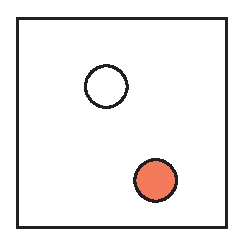
\includegraphics[width=1.5in]{sample.eps}
%  \caption{Lookit! Lookit!}
%}

%% Abstract section.
\abstract{
%
We present a study of a tangible user interface for architectural
design and daylighting analysis.  This tool provides an intuitive way
for architects and future occupants to quickly construct physical
models and then view a simulation of daylighting in the model at
interactive rates.
%
%\fbo{blah sentence}
%User studies are an effective way to obtain both qualitative and
%quantitative feedback for user interfaces.
%
We conducted a user study of both formally-trained architects and
non-architects in a set of analysis and design exercises.
%
This study investigates the effectiveness of this interface as an
educational tool, the precision and accuracy of the constructed
physical models, and the overall effectiveness of the tangible
interface.  The four part study investigates users' intuitions about
daylighting and their interaction with the tool for analysis of an
existing space, for proposing renovations to the space, and for
designing a totally new space with the same architectural program that
better addresses the occupants' needs.  These exercises revealed
misconceptions in many of the participants' intuitions about
daylighting and overall the participants expressed interest in this
simulation tool for daylighting analysis in architectural design.
%
} % end of abstract

%% ACM Computing Classification System (CCS). 
%% See <http://www.acm.org/class/1998/> for details.
%% The ``\CCScat'' command takes four arguments.

\CCScatlist{ 
  \CCScat{H.5.2}{Information Interfaces and Presentations}%
{User Interfaces}{Evaluation/methodology};
  \CCScat{I.3.7}{Computer Graphics}{Three-Dimensional Graphics and Realism}{Virtual Reality}
}

%% Copyright space is enabled by default as required by guidelines.
%% It is disabled by the 'review' option or via the following command:
% \nocopyrightspace

%%%%%%%%%%%%%%%%%%%%%%%%%%%%%%%%%%%%%%%%%%%%%%%%%%%%%%%%%%%%%%%%
%%%%%%%%%%%%%%%%%%%%%% START OF THE PAPER %%%%%%%%%%%%%%%%%%%%%%
%%%%%%%%%%%%%%%%%%%%%%%%%%%%%%%%%%%%%%%%%%%%%%%%%%%%%%%%%%%%%%%%%

\renewcommand{\topfraction}{0.99}
\renewcommand{\bottomfraction}{0.99}
\renewcommand{\textfraction}{0.1}
\renewcommand{\floatpagefraction}{0.99}

\begin{document}

%% The ``\maketitle'' command must be the first command after the
%% ``\begin{document}'' command. It prepares and prints the title block.




%% the only exception to this rule is the \firstsection command
\firstsection{Introduction}
\maketitle


Architectural daylighting design is the use of windows and reflective
surfaces to make effective use of natural light from the sun and sky
within a physical environment.  Increased use of daylighting can
reduce the need for supplemental electric lighting during the day,
decreasing operating costs and reducing the consumption of
non-renewable resources.  Furthermore, the dynamic time-varying and
seasonally-varying qualities of daylighting can make spaces with
natural light more interesting and comfortable.  However, the
distribution of daylighting within a building for a particular moment
can be difficult for non-experts to accurately and quantitatively
predict, and detailed simulations are expensive.  In a common design
scenario for an office space, the typical goals for daylighting are to
maximize the {\em daylight autonomy}, the number of hours per day/year
that the work surfaces receive adequate lighting for reading.  Yet too
much sunlight is also problematic: we must avoid the possibility of
{\em glare}, reduced visibility for occupants of the space due to high
contrast in light intensity within the visual field.
%
The tight integration of daylighting and architectural form split late
in the twentieth century~\cite{lechner2001heating}.  Up to that point,
maximizing total window area was a major goal in design.  To ensure
all areas in the building had sufficient access to daylighting, most
buildings were less than 60' wide.  With the increased availability of
cheap artificial lighting, daylighting became more of an afterthought
in architecture.  Recent concerns about energy consumption and a new
emphasis on aesthetic choices have re-invigorated interest in
daylighting analysis.

% and motivated our daylighting simulation tool for
%architectural designs~\cite{ShengYYC09}
%(Figure~\ref{figure:tabletop}).
%In this paper we evaluate this Spatially Augmented Reality (SAR)
%system; a concept first introduced by {\em Shader Lamps} to project information
%onto existing surfaces in the real world~\cite{Raskar:2001:SLA}.

\begin{figure}[t]
  \centering
  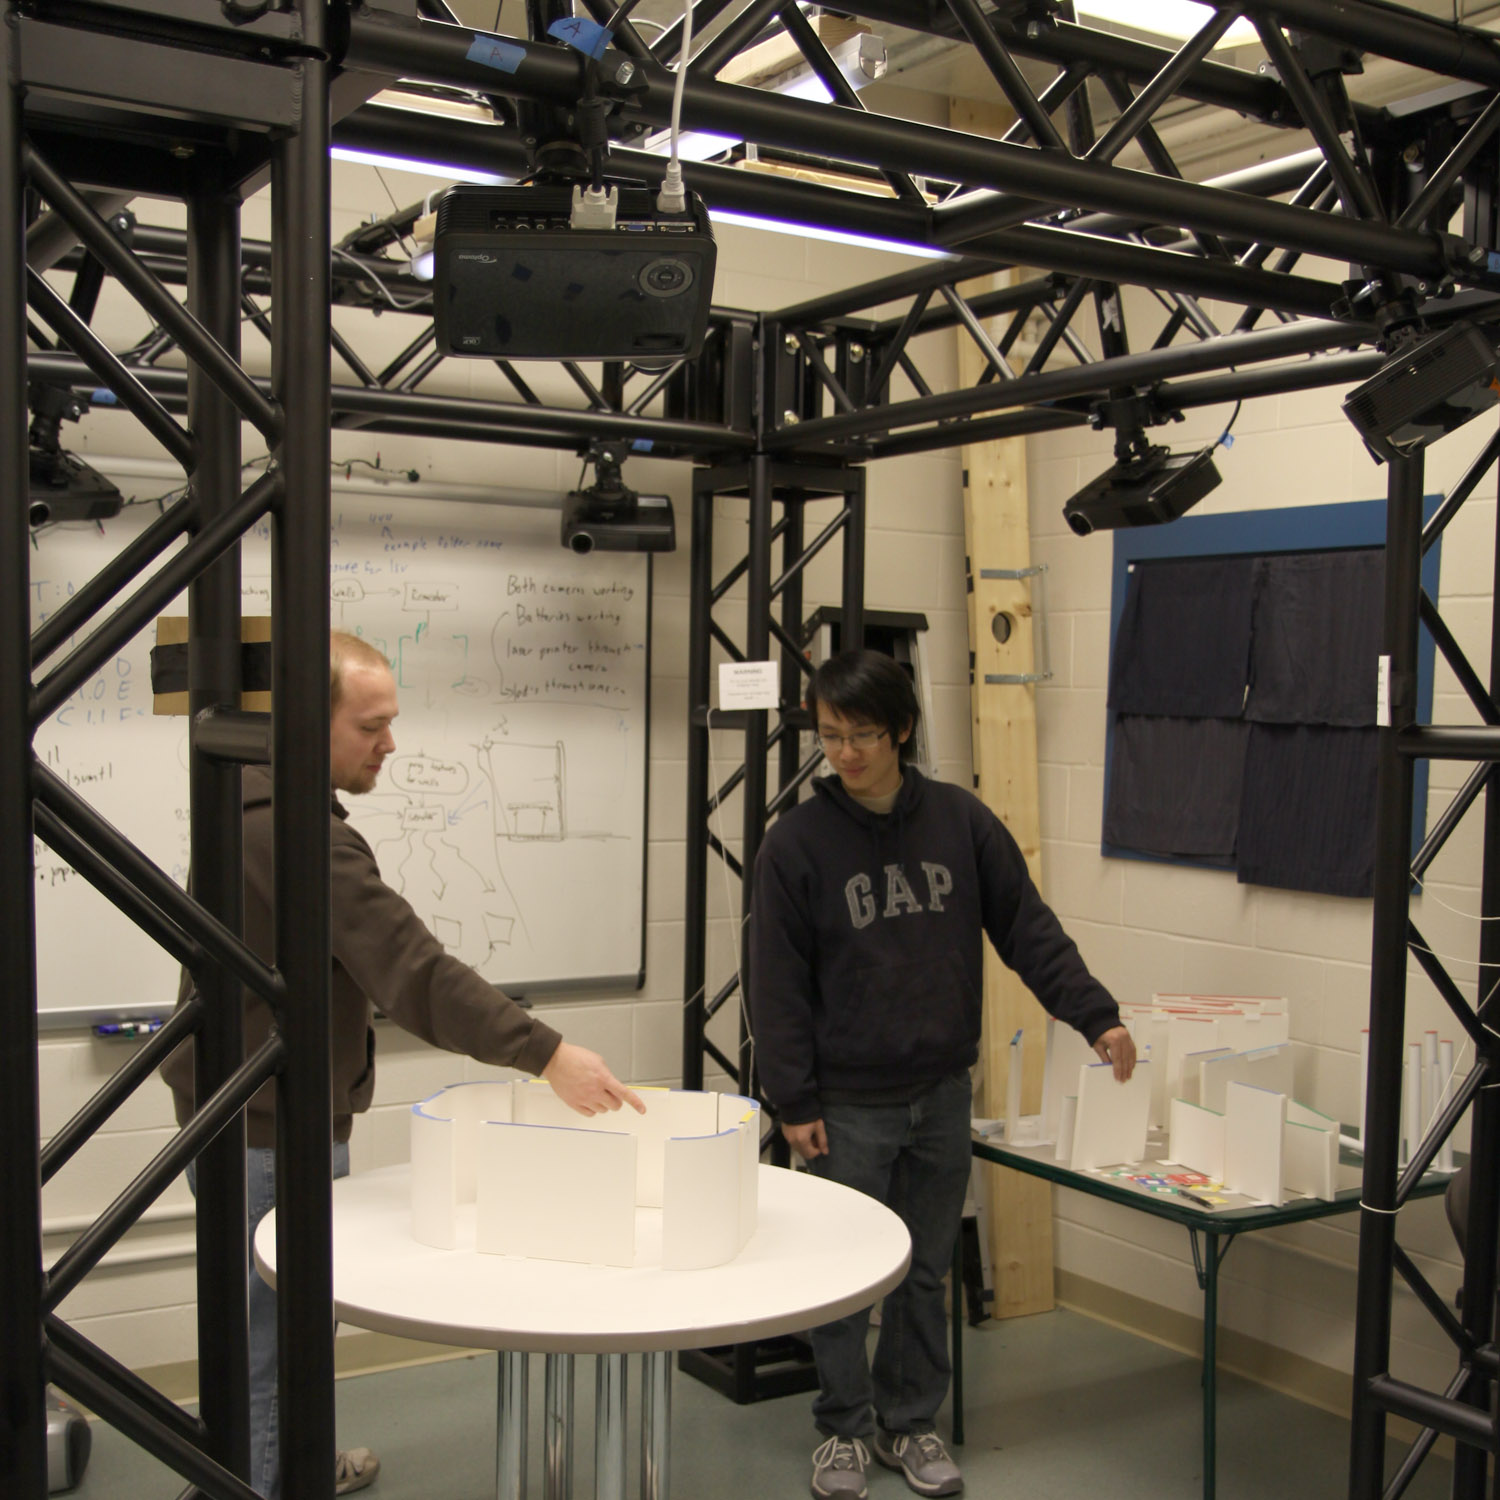
\includegraphics[width=1.65in]{images/photos/josh_jonathan_new_contraption}
  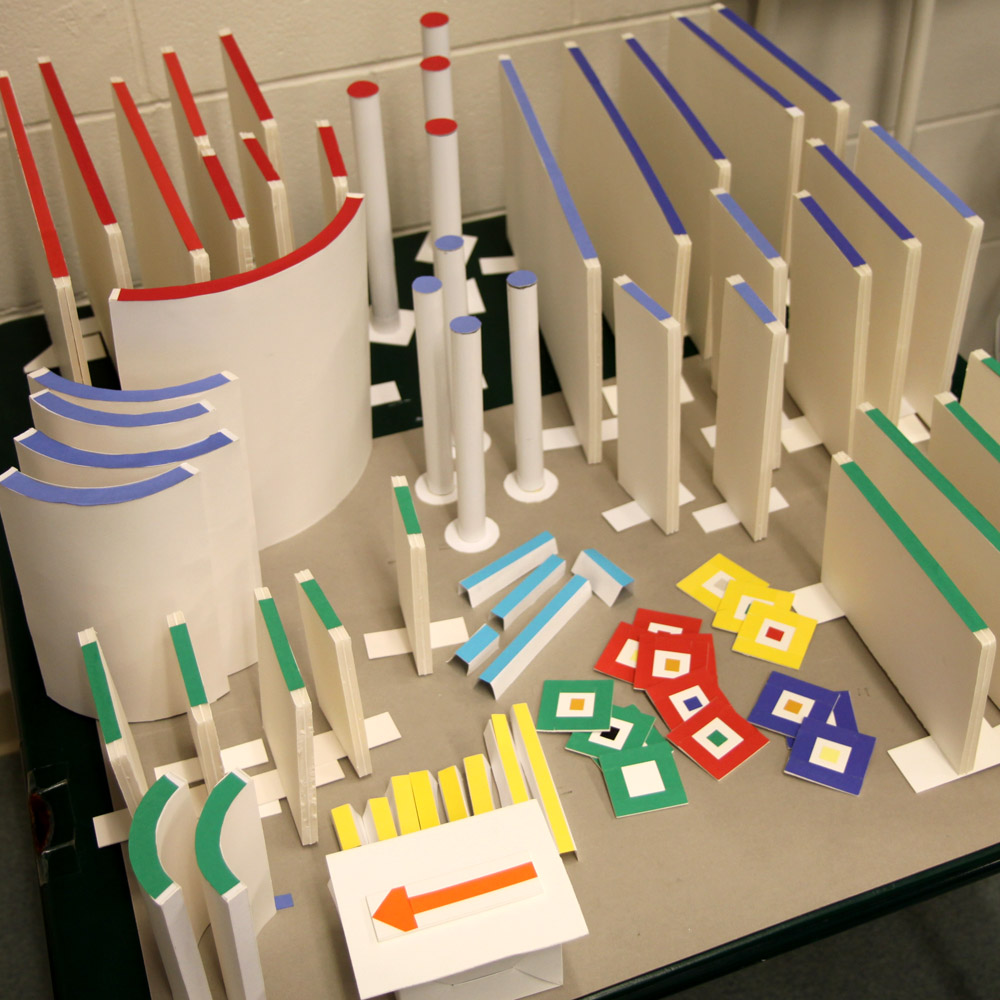
\includegraphics[width=1.65in]{images/photos/available_wall_pieces}\vspace{-0.19in}\\
\begin{minipage}{1.65in}~{\color{white}{\bf a)}}\end{minipage}
\begin{minipage}{1.65in}~{\color{white}{\bf b)}}\end{minipage}\vspace{0.05in}\\
  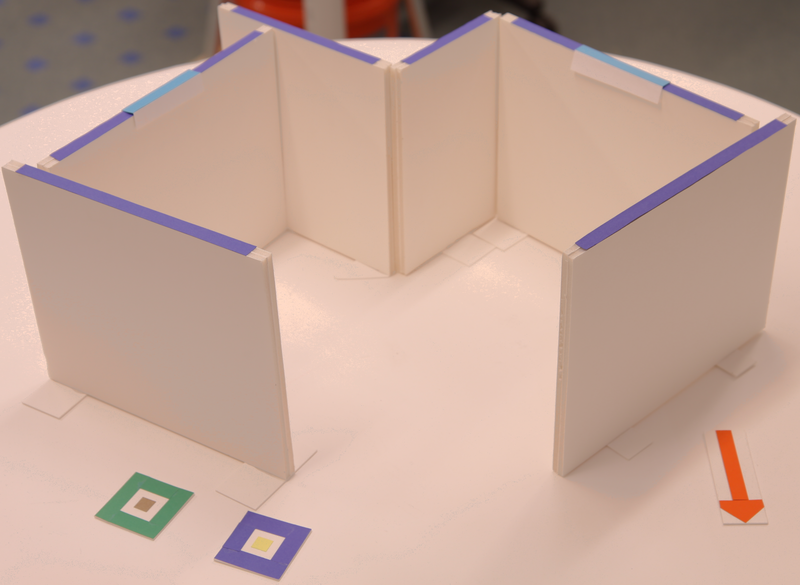
\includegraphics[width=1.65in]{images/photos/sample_model}
  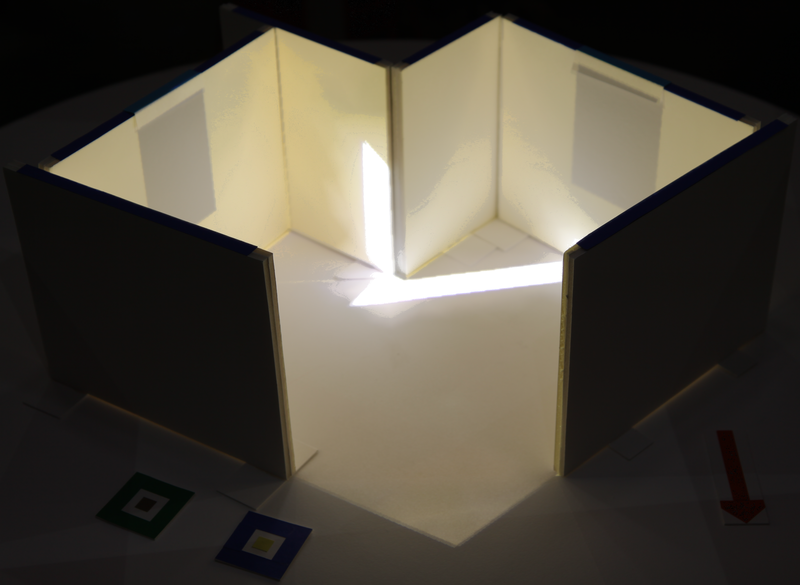
\includegraphics[width=1.65in]{images/photos/sample_rendering}\vspace{-0.19in}\\
\begin{minipage}{1.65in}~{\color{black}{\bf c)}}\end{minipage}
\begin{minipage}{1.65in}~{\color{white}{\bf d)}}\end{minipage}\vspace{-0.00in}\\
  \caption{Our new TUI for architectural daylighting design allows
    multiple users to a) gather around a physical sketching
    environment and select from b) a set of wall primitives and window
    and material markers to c) build a rough sketch of an
    architectural design.  A d) visualization of a daylighting
    simulation is projected onto these surfaces. }
\vspace{-0.1in}
  \label{figure:tabletop}
\end{figure}




In this paper we evaluate a new tangible interface for architectural
daylighting analysis (Figure~\ref{figure:tabletop}).  This system is a
form of Spatially Augmented Reality (SAR) first introduced by
\emph{Shader Lamps} as a way to project information onto existing
surfaces in the real world~\cite{Raskar:2001:SLA}.  The daylighting
analysis system simulates the complex inter-reflection of natural
light within a scene and uses a series of projectors surrounding the
table to ``paint'' the physical primitives with the simulation
results.  Designing in the tabletop system is done by sketching with
physical \emph{wall primitives} that are detected and interpreted to
create a closed space.  The overall orientation of the sketch is
specified with a \emph{north arrow primitive}, windows in the model
are positioned by slipping \emph{window primitives} over the top edge
of the walls, and surface material properties (color) are indicated
with small tokens.  Users are limited to these specific primitives and
markers to ensure that the sketching interface is intuitive and
easy-to-use.
%While more complex primitives could be
%added, it would require more advanced computer vision techniques and
%the system could become less effective as a sketching tool.
%
A calibrated overhead camera captures the arrangement of these
elements and 
%computer vision techniques are used to detect the
%complete model.  
the geometry is converted into a closed triangle mesh.  Radiosity, a
patch-based lighting method, is used to simulate light propagation
within the space and the rendering system displays the simulated
natural lighting on the physical model using six projectors positioned
in a circle above the table.  The system provides two different
daylighting visualization modes: a static time and a dynamic
time-lapse animation for a whole day.  The lighting simulation can be
done for any day of the year.


Our tool is intended for use in the earliest stages of architectural
design, when the orientation of the building on the site, the relative
positions of rooms within the building, the proportions of the rooms,
and the placement and shape of windows is not yet determined.
Existing commercial software for daylighting simulation focuses on
more polished and complete designs.  It can take significant time
(from minutes to hours) for the designer to construct a digital model
that both captures the current design and is suitable for accurate and
efficient simulation.  Our tangible interface takes just seconds to
build or edit a model and thus is appropriate for rough sketching and
brainstorming with quick, online evaluation of building performance.
Once the design is fixed and the details fleshed out, the designer is
ready to run the detailed simulations available with current software
packages.  We envision our tool being useful for a wide audience.  Not
only will it be useful for architecture students and professional
architects, but also for interior designer and future occupants
working on tasks such as furniture placement.

%This paper describes our initial user study of this interface with
%thirteen student participants: six architecture majors and seven
%non-architects (five of which have some general design training).
%, 7 non-architectsze of the
%students were architecture students and 7 were non-architecture
%students with 5 of them having some design training.
%


















%% \section{Introduction} 
%Architectural daylighting design is the use of windows and reflective
%surfaces to make effective use of natural light from the sun and sky
%within a physical environment.  Increased use of daylighting can
%reduce the need for supplemental electric lighting during the day,
%decreasing operating costs and reducing the consumption of
%non-renewable resources.  Furthermore, the dynamic time-varying and
%seasonally-varying qualities of daylighting can make spaces with
%natural light more interesting and comfortable.  However, the
%distribution of daylighting within a building for a particular moment
%can be difficult for non-experts to accurately and quantitatively
%predict, and detailed simulations are expensive.  In a common design
%scenario for an office space, the typical goals for daylighting are to
%maximize the {\em daylight autonomy}, the number of hours per day/year
%that the work surfaces receive adequate lighting for reading.  Yet too
%much sunlight is also problematic: we must avoid the possibility of
%{\em glare}, reduced visibility due to high contrast in light
%intensity within the visual field, for occupants in the space.
%%
%Late in the twentieth century daylighting and architecture began to be
%considered separately~\cite{lechner2001heating}.  Up to that point, a
%major part of architecture had been trying to make as many large
%windows as possible.  Before this time most buildings were 60 feet
%wide or less so that all parts of a building would be close to a
%window.  Because of the availability of cheap artificial lighting more
%recently, daylighting has become more of an afterthought in
%architecture.  

%Recent concerns about energy consumption as well as
%more emphasis on aesthetic choices have motivated us to make a
%daylighting simulation tool for architectural designs\fbox{anonymous,
%  ugh}
%~\cite{ShengYYC09} 
%as seen in Figure 
%
%
%In this paper we evaluate a new tangible interface for architectural
%daylighting analysis (Figure~\ref{figure:tabletop}).
%this tool.  
%This system is a form of Spatially Augmented Reality (SAR) first
%introduced by \emph{Shader Lamps} as a way to project information onto
%existing surfaces in the real world~\cite{Raskar:2001:SLA}.
%
%Our tool is intended for use in the earliest stages of architectural
%design, when the orientation of the building on the site, the relative
%positions of rooms within the building, the proportions of the rooms,
%and the placement and shape of windows is not yet determined.
%
%In the architectural design process, the effect of
%daylight in the space is often treated as an afterthought.
%
%Existing commercial software for daylighting simulation focuses on
%more polished and complete designs.  It can take significant time
%(from minutes to hours) for the designer to construct a digital model
%that both captures the current design and is suitable for accurate and
%efficient simulation.
%
%and digital model files.
%
%lighting simulation methods available require a model to be
%built prior to any lighting test.  This interface is designed to
%change the process so that lighting simulation can be done hand in
%hand with the sketching process.  
%Our tangible interface takes just seconds to build or edit a model and
%thus is appropriate for rough sketching and brainstorming with quick,
%online evaluation of building performance.
%
%Our interface is intended for early stage rough modeling Our interface
%does well to simulate themes in lighting simulation, 
%Once the design is fixed and the details fleshed out, the designer is
%ready to run the detailed simulations available with current software
%packages.
%ill be run later with a more precise model.  Because
%of the prior simulation only minor modifications should be necessary
%after the detailed simulation. \fbox{right spot? maybe conclusion}

%The daylighting analysis system simulates the complex inter-reflection
%of natural light within a scene and uses a series of projectors surrounding
%the table to ``paint'' the physical primitives with the simulation
%results.  Designing in the tabletop system is done by sketching with
%physical \emph{wall primitives} which are detected and
%interpreted to create a closed space.  The overall orientation of the
%sketch is specified with a \emph{north arrow primitive}, windows in
%the model are specified by \emph{window primitives} which can be
%slipped over the top edge of the walls and material properties (color)
%for the surfaces of the model are specified with small physical
%tokens.  Users are limited to these specific primitives and markers
%with the goal of ensuring the system is easy to use and remains a
%simple and robust sketching interface.
%While more complex primitives could be
%added, it would require more advanced computer vision techniques and
%the system could become less effective as a sketching tool.
%
%A calibrated overhead camera captures the arrangement of these
%elements and computer vision techniques are used to detect the complete model.
%This geometry is converted into a triangle mesh and a patch-based
%lighting method, radiosity, is used to simulate light propagation
%within the space.  The rendering system displays the simulated natural
%lighting in the room using six projectors positioned in a circle above
%the table.
%
% Is this too redundant
%The wall primitives used on the tabletop are rectangular pieces of
%foam core with cardboard feet.  Three different heights of walls are
%available in the system; these heights are differentiated by distinct
%colors for each wall height.  A single camera, mounted approximately
%seven feet above the tabletop is sufficient for the system because all
%of the primitive's heights can be inferred from the color of the
%walls.  Window markers (made of colored pieces of index cards) can be
%fitted over the tops of walls to indicate where windows are desired.
%The system has two different colored window markers allowing the user
%to specify and differentiate multiple instances of two types of
%windows.

%Two additional types of tokens are used to specify the model.  The
%orange north arrow primitive indicates the orientation of the building
%on the site.  Furthermore, the materials of the model are communicated
%to the system by 3 additional tokens: wall markers, floor markers, and
%ceiling markers, which are differentiated from each other by the
%border color. A paint chip in the center of the token indicates the
%color of the material.  



%The system provides two different daylighting visualization modes:
% of the daylighting
%simulation: 
%a static time and a dynamic time-lapse animation for a whole day.  The
%lighting simulation can be done for any day of the year.  The location
%on the earth and the sky model can be specified for the daylighting
%simulation software.
%%
%The system provides a comprehensive sketching tool for architectural
%design while allowing users to effectively simulate daylight in the
%space.  
%
%We envision our tool being useful for a wide audience.  Not only will
%it be useful for architecture students and professional architects,
%but also for people using buildings with natural daylighting for tasks
%such as furniture placement.
%
%Preliminary user studies were an using this interface. 
%This paper describes a studour initial user study on this interface with
%thirteen student participants: six architecture majors and seven
%non-architects (five of the non-architecture majors have some general
%design training).
%, 7 non-architectsze of the
%students were architecture students and 7 were non-architecture
%students with 5 of them having some design training.
%

\noindent
The contributions of our paper: \vspace{-0.1in}

\begin{itemize}


\item Exploration of participants' fundamental understanding of
  daylighting design, overlighting, underlighting and glare.\vspace{-0.1in}

\item Quantitative analysis of the users' accuracy in using our
  physical sketching system to model a room they had just visited.\vspace{-0.1in}

\item Evaluation of the participants' use of our tool and their
  perception of quantitative and qualitative daylighting from the 
  displayed simulations.\vspace{-0.1in}

\item Demonstration of our tangible interface as a
  creativity-enhancing tool for architectural daylighting design.


\end{itemize}


%\vspace{-0.05in}
\section{Related Work}
%\vspace{-0.05in}

%In evaluating a Tangible User Interface for an Augmented reality
%system many Interfaces were influential.
%\fbox{add paper about lighting model/accuracy}
%done...or at least started\fbox{can we frame these in terms of Design, Accuracy, and education?}
%\fbox{media lab papers?}

Three prevalent themes in the field of Tangible User Interfaces (TUIs)
are education, accuracy, and design.  
%While these themes clearly
%intersect, each one must be carefully addressed when designing and
%evaluating an interface.  
The novel interactions made available by TUIs make them exciting
candidates for alternate teaching techniques.  Furthermore, since TUIs
feature list includes
%are used for things including 
point and click interactions, layout design, and simulation, the
accuracy of both the user's input and the user's perception of the
output must be evaluated.  Since architecture is a design process of a
tangible structure, many TUIs have focused on design tasks.


%Three prevalent themes in the field of Tangible User Interfaces (TUIs)
%are education, accuracy, and design.  While these themes clearly
%intersect, each one must be carefully addressed when designing and
%evaluating an interface.  The novel interactions made available by
%TUIs make them exciting candidates for alternate teaching techniques.
%Furthermore, since TUIs feature list includes 
%are used for things including 
%point and click interactions, layout design, and simulation, the
%accuracy of both the user's input and the user's perception of the
%output must be evaluated.  Since architecture is a design process of a
%tangible structure, TUIs are popular 
%have been used extensively 
%in this context.
%e design
%process

%Several design interfaces are
%presented in this section. 

%\vspace{-0.05in}
\subsection{Education/Information Tools}
%\vspace{-0.05in}

TUIs inspire innovation in teaching and learning 
%in innovative ways because of the
through the opportunity to physically interact with data.
%
Ishii and Ullmer present an interface of {\em phicons} (physical
icons) and multiple display surfaces to navigate campus information.
They combine a backprojected display and an LCD screen to create the
%that they
%refereed to as 
{\em activeLENS}, which allows users to view an overview map and 3D
information~\cite{Ishii97tangiblebits:}.
%
Yee created a hybrid of this interface with a traditional interface
%, Yee
%created 
for a workspace with a large passive 
%(large non-interactive) 
display and a smaller handheld display for 
%which allowed for 
stylus input~\cite{642613}.  Unlike the activeLens, this system
effectively utilizes both hands for data manipulation: one to hold and
guide the lens and one for stylus input.  Maekawa
%Developed a system
extended the 
%that used a similar display to the 
ActiveLens-style display to
%, but where the input was
a the surface of re-configurable blocks.  This display system maps the
current 3D configuration to a database of shapes
% to the configuration of
%blocks and 
and displays on a small mobile screen the appropriate ``window'' into
the corresponding virtual object~\cite{1517704}.  Jacob et
al. developed the first system to directly project onto movable,
tangible {\em pucks} for data manipulation~\cite{Jacob01atangible}.
%segment
%shapes.  
%n interface that could project on
%objects that users could manipulate~\cite{Jacob01atangible}.  By
%moving \emph{pucks} users could segment 
%data into different groups (for instance grouping employees when
%scheduling them).  
%The puck interface was one of the first to allow the projection
%surfaces themselves to be manipulated in a similar way to how we now
%project on the walls of users designs.  
Spindler developed PaperLens~\cite{Spindler:2009:PAM:1731903.1731920},
an interface using a tangible 2D display to show 3D information.
%The
%PaperLens ~\cite{Spindler:2009:PAM:1731903.1731920} allowed a paper to
%be moved through 3-D space and have either layers of 2-D information
%or 3-D information be projected upon it based on the position.
Similarly, Song presents a tangible interface with a touch screen for
%that
displaying
%displays 
select planes of data based on its orientation relative to a large 2D
display~\cite{Song:2011:WEA:1978942.1979140}.
%relative on where it was touching a large 2-D
%display and the orientation of the touch screen
%
As illustrated by these TUIs and others, displays allowing physical
manipulation provide unique opportunities to visualize, organize,
and understand data.
%that were not previously available. 
%Education is a field that is particularly well suited to alternate
%ways to communicate information visually.



%TUIs can aid education in innovative ways because of the opportunity
%to physically interact with data. 
%
%Ishii and Ullmer presented an interface that used phicons (physical
%icons) and multiple display surfaces to navigate campus information.
%They combined a backprojected display and an LCD screen to create the
%that they
%refereed to as 
%{\em activeLENS}, allowing users to view an overview map or
%view 3D information with this device~\cite{Ishii97tangiblebits:}.
%
%Yee created a hybrid of this interface with a traditional interface
%, Yee
%created 
%for a workspace that had a passive (large non-interactive) display
%with a handheld display which allowed for stylus input~\cite{642613}.
%Unlike the activeLENS, this system effectively utilized both hands for
%data manipulation: one to hold and guide the lens and one for stylus
%input.  Maekawa developed a system that used a similar display to the
%activeLENS, but where the input was a configuration of tangible
%blocks.  This display system would discern the closest 3D shape in a
%database to the configuration of blocks and display on a small digital
%screen a window into the corresponding virtual object based on the
%actual physical position~\cite{1517704}.  The MIT Media Lab developed
%an interface that could project on objects that users could
%manipulate~\cite{Jacob01atangible}.  By moving \emph{pucks} users
%could segment data into different groups (for instance grouping
%employees when scheduling them).  The puck interface was one of the
%first to allow the projection surfaces themselves to be manipulated in
%a similar way to how we now project on the walls of users designs.
%Spindler developed one interface which used a tangible 2-D display to
%show 3-D information.  The PaperLens
%~\cite{Spindler:2009:PAM:1731903.1731920} allowed a paper to be moved
%through 3-D space and have either layers of 2-D information or 3-D
%information be projected upon it based on the position.  Similarly,
%Song developed a tangible interface that had a touch screen which
%could display planes of data based on where it was touching a large
%2-D display and the orientation of the touch screen
%~\cite{Song:2011:WEA:1978942.1979140}.

%As illustrated by these TUIs and others, displays which can be physically manipulated provide unique opportunities to group and handle data that were not previously available. Education is a field that is particularly well suited to alternate ways to communicate information visually.

%\vspace{-0.05in}
\subsection{Accuracy/Usability}
%\vspace{-0.05in}

The usefulness of TUIs is directly correlated to the ability to
%are  only end up being useful insofar as they can
correctly and fully recognize data expressed by the user and likewise
accurately convey important information.
%
The \emph{Digital Desk}~\cite{159630}
used a projector and camera to create a hybrid desk
surface-computer desktop interface.  Data could be manipulated and
collected in the computer by writing and interacting with information
on the table surface.  This desk enabled remote users to work on
the same virtual surface, making accurately collecting and projecting information 
important for effective interaction.
%
An important sub-field of TUIs is 
%As TUI's developed an important subfield became 
{\em graspable interfaces}, for example, 
%, which allow users to tangibly interact
%with a system by tangible controls.  
the ``Bricks''
system~\cite{223964}, which utilized multiple graspable controls
%that could be used 
in tandem to select or expand information.  
%As with the Bricks system,
To ensure the usefulness and precision of the application, it is
imperative that the graspable or tangible interface accurately and
precisely detect the user's actions.

In addition to accurately responding to interactions, usability is a
prime concern.  A user study on the map viewing tool, ``Like Bees
around the Hive''~\cite{1518991}, found that users enjoyed the
% using the
tool, but were less adept at performing a specific task
%their task 
%using it 
when compared to a traditional digital map interface.  Even though
the data displayed was
accurate, the interface was not effective because of usability
concerns involving specific types of interactions.  Similarly in our interface not only must data be
displayed accurately, but it also must be displayed in a manner in
which users can intuitively understand the displayed information.



%The usefulness of TUIs is directly correlated to their ability to
%are  only end up being useful insofar as they can
%correctly and fully recognize data communicated to them and accurately
%convey information back to the user.
%
%One of the earliest TUIs was the \emph{Digital Desk}~\cite{159630},
%which used a projector and camera to create a hybrid desk
%surface-computer desktop interface.  Data could be manipulated and
%collected in the computer by writing and interacting with information
%on the table surface.  This desk enabled remote users to work on the
%same virtual surface and allowed applications like a calculator that
%were projected on the desk.  While not the primary concern in the prototype they developed, accuracy c%ollecting and projecting information was important for remote interaction to be useful. 

%An important sub-field of TUIs is 
%As TUI's developed an important subfield became 
%{\em graspable interfaces}, which allow users to tangibly interact
%with a system by tangible controls.  The ``Bricks'' system~\cite{223964} utilized
%multiple graspable controls 
%%that could be used 
%in tandem to select or expand information.  As with the Bricks system,
%accurately detecting the interactions of the user is imperative for
%many Tangible Interfaces for them to be useful and precise.%

%In addition to accurately responding to interactions, usability is a
%prime concern.  A user study on the map viewing tool, ``Like Bees
%around the Hive''~\cite{1518991}, found that users enjoyed the
%% using the
%tool, but were less adept at performing a specific task
%%their task 
%%using it 
%when compared to a traditional digital map interface.  Even though
%there was no evidence to suggest that the data displayed was
%inaccurate, the interface was not effective because of usability
%concerns involving specific types of interactions.
%We have a similar usability concern with our user interface; not only must data be displayed accuratel%y, but it also must be displayed in a manner in which users can intuitively understand the displayed information.

%\vspace{-0.05in}
\subsection{Design}
%\vspace{-0.05in}

%As the field of Tangible User Interfaces has advanced, a variety of
%design tools have been demonstrated for different application areas.
%%many design
%%tools have been proposed.  
%Lucchi et al. ran a user study comparing design interaction on two tabletop
%surfaces with different interaction techniques: tangible interaction and touch interaction~\cite{1709917}. In their comparison, in which they allowed full functionality of both interfaces, the tangible interface allowed users to perform tasks more quickly.  This comparison assumed fully functional interfaces for both systems and not simply the least common denominator of a tangible and multi-touch interface.
%\fbox{work in better?}The luminous-tangible workbench~\cite{Urp99urp:a} provided a tangible interface %for urban planning.  It showed the shadows buildings cast upon one another, but did not simulate lighting in interior spaces.

%As was the case with these interfaces 
%When validating TUIs through user studies, researchers must be sure
%to frame questions appropriately and to be clear how a comparison between inherently different interfa%ces is done.
%%the questions they ask are framed in the best method possible.  
%Many tools have been developed which are designed to both be an informative tool as well as to encourage creativity.
%
%The JUMP tool~\cite{1268540} rectifies multiple architectural documents (e.g.,
%electrical and mechanical) for a construction project.  The prototype
%interface involves placing a different token on the workspace to view
%each document.  A formal user study of this tool revealed that often
%the users felt as if they were in a foreign environment with these
%primitives and preferred a more traditional way (mouse and keyboard)
%to interact with the same information.  Thus, in our study we seek to
%answer if our novel daylighting interface is beneficial or if our
%users prefer traditional interfaces.



\begin{figure}[t]
\centering
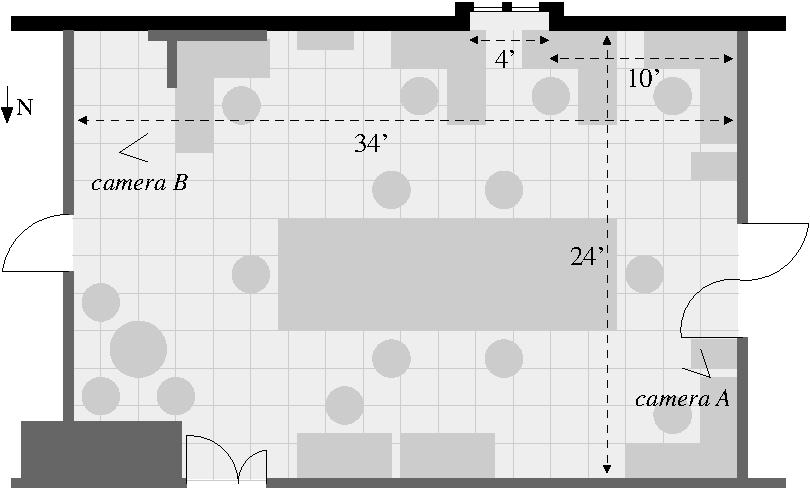
\includegraphics[width=2.5in]{images/lab.pdf} \vspace{0.1in}
\\
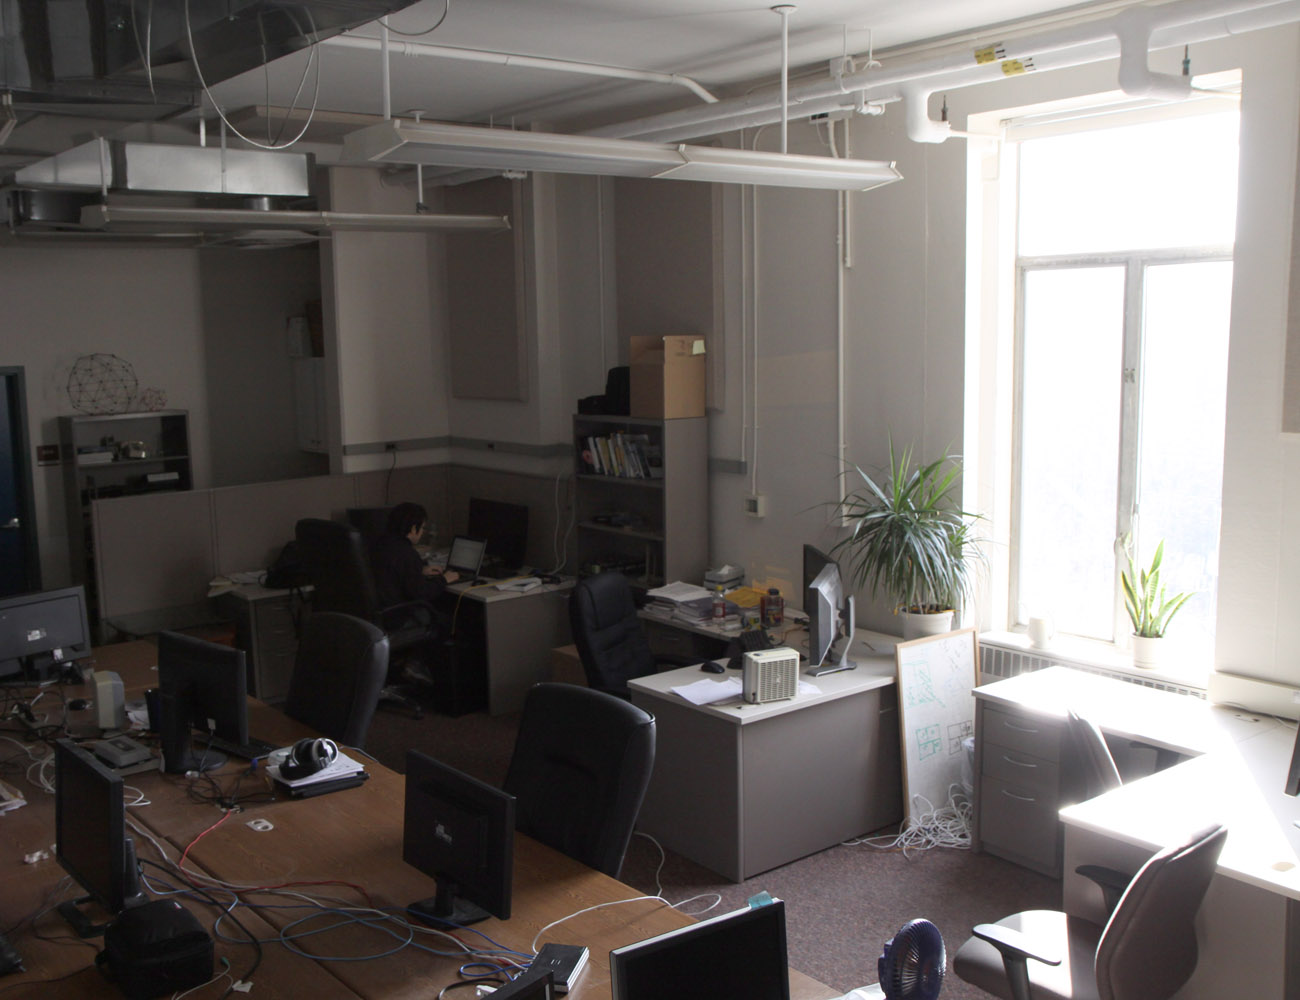
\includegraphics[width=1.65in]{images/photos/camera_angle_2_lights_off.jpg}
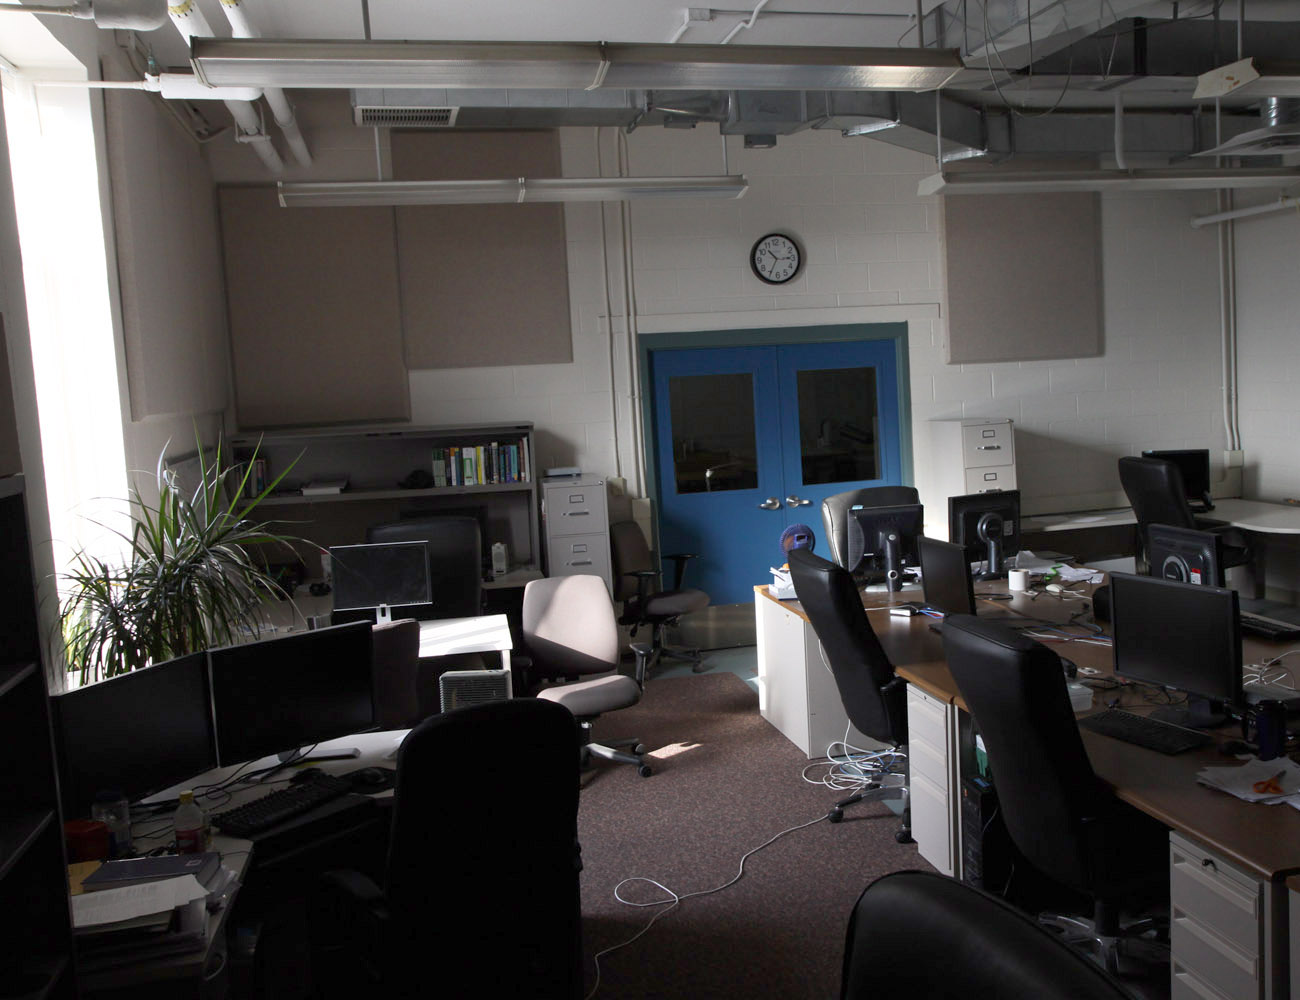
\includegraphics[width=1.65in]{images/photos/camera_angle_3_lights_off.jpg}\vspace{-0.19in}\\
\begin{minipage}{1.65in}~{\color{white}{\em camera A, lights off}}\end{minipage}
\begin{minipage}{1.65in}~{\color{white}{\em camera B, lights off}}\end{minipage}\vspace{0.05in}\\
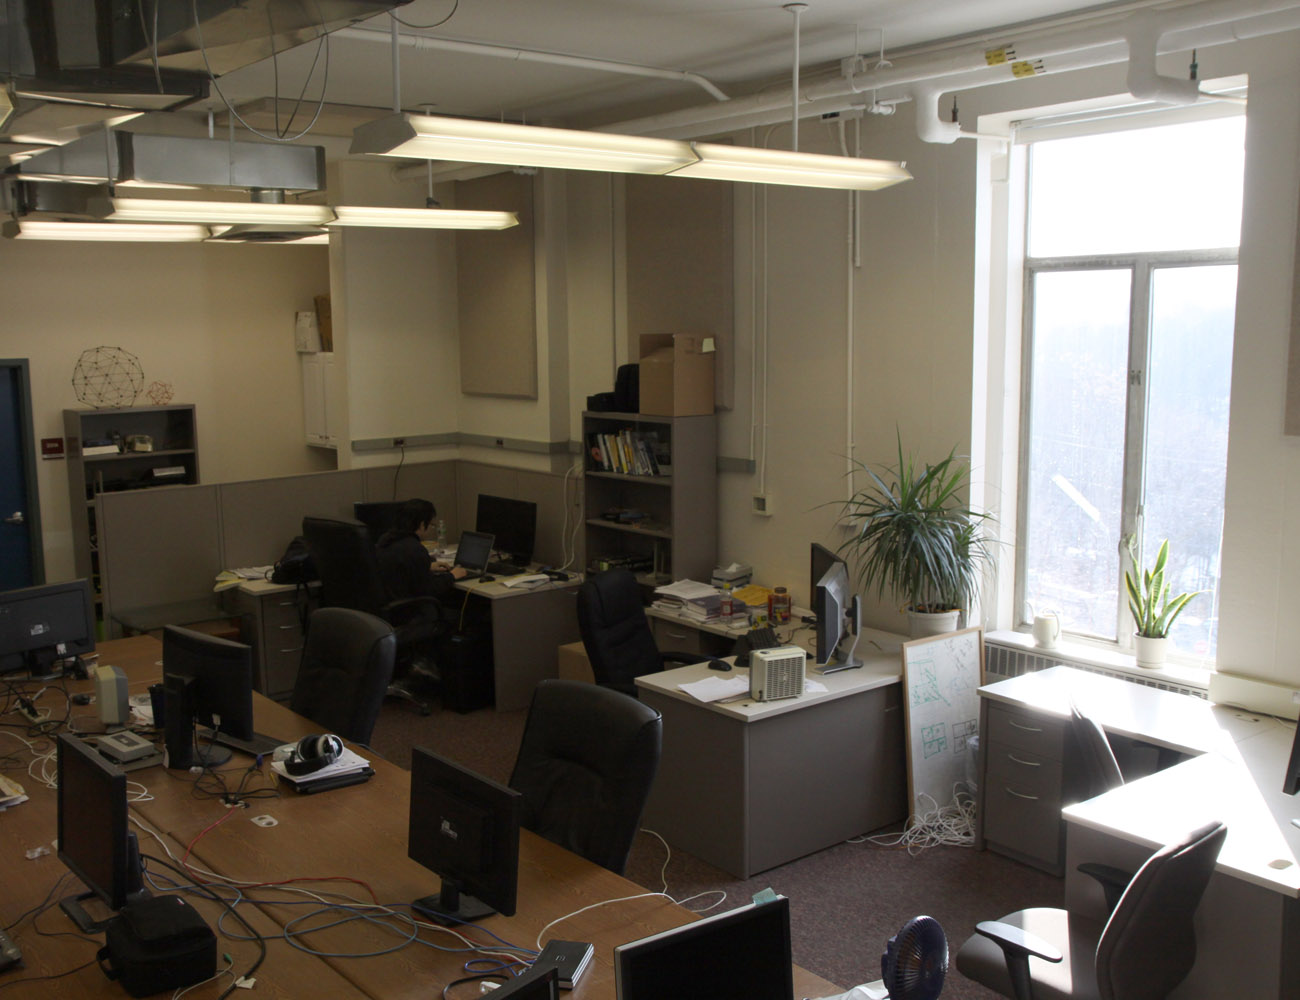
\includegraphics[width=1.65in]{images/photos/camera_angle_2_lights_on.jpg}
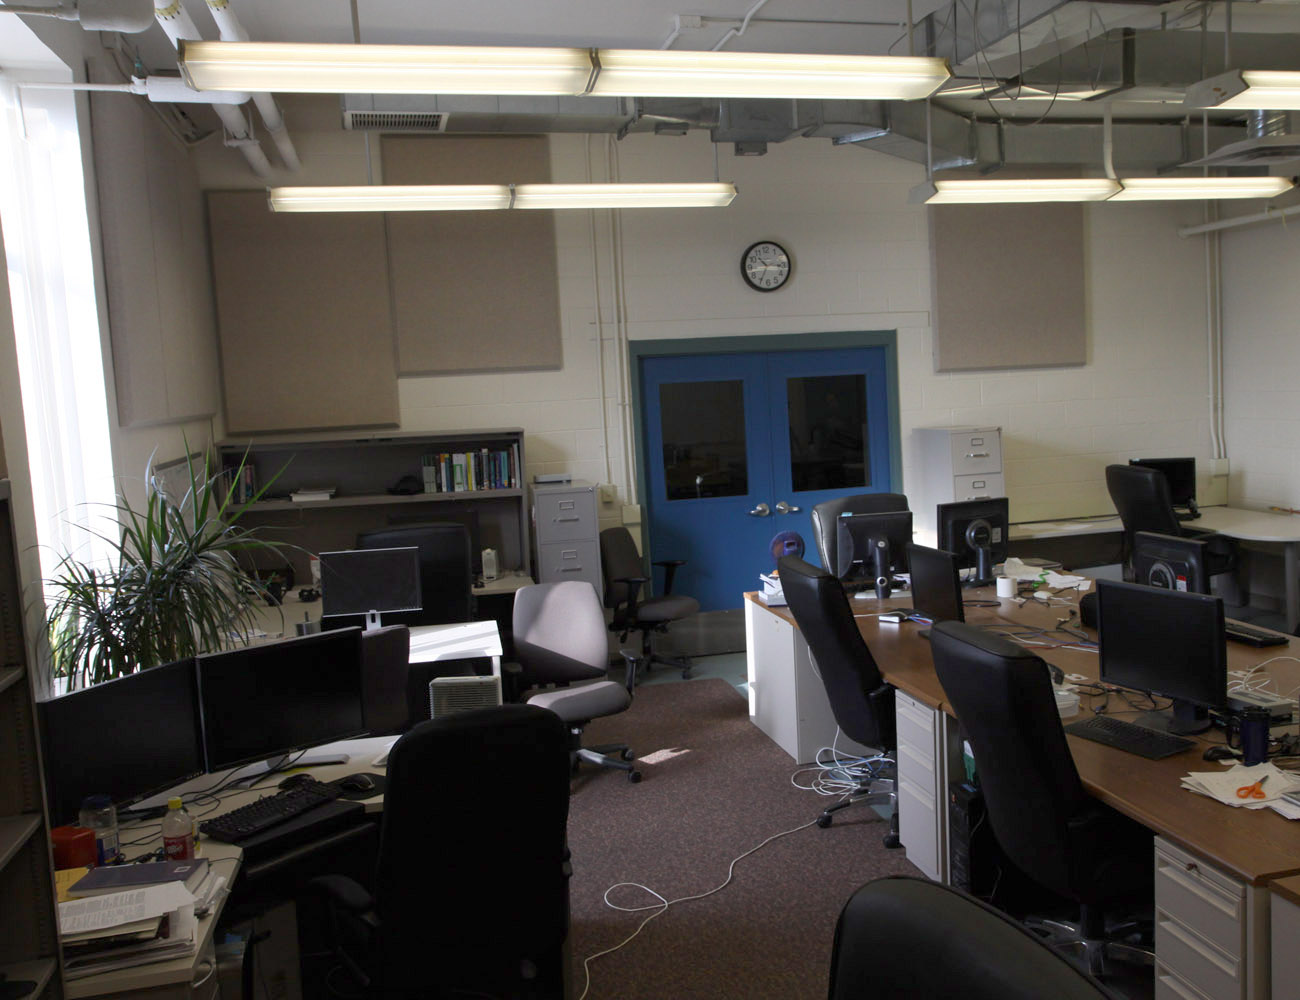
\includegraphics[width=1.65in]{images/photos/camera_angle_3_lights_on.jpg}\vspace{-0.19in}\\
\begin{minipage}{1.65in}~{\color{white}{\em camera A, lights on}}\end{minipage}
\begin{minipage}{1.65in}~{\color{white}{\em camera B, lights on}}\end{minipage}\vspace{0.00in}\\
\caption{User study participants visited this simple open office
  environment as a case study for daylighting analysis.  The room
  contains a single, tall and narrow, south-facing window that
  provides direct overly-intense illumination to portions of the room
  while leaving other areas relatively dark.  Thus, occupants of the
  space typically turn on the overhead lights, even on sunny
  afternoons.
}
\label{figure:example_room}
\end{figure}


\begin{figure*}[t]
%
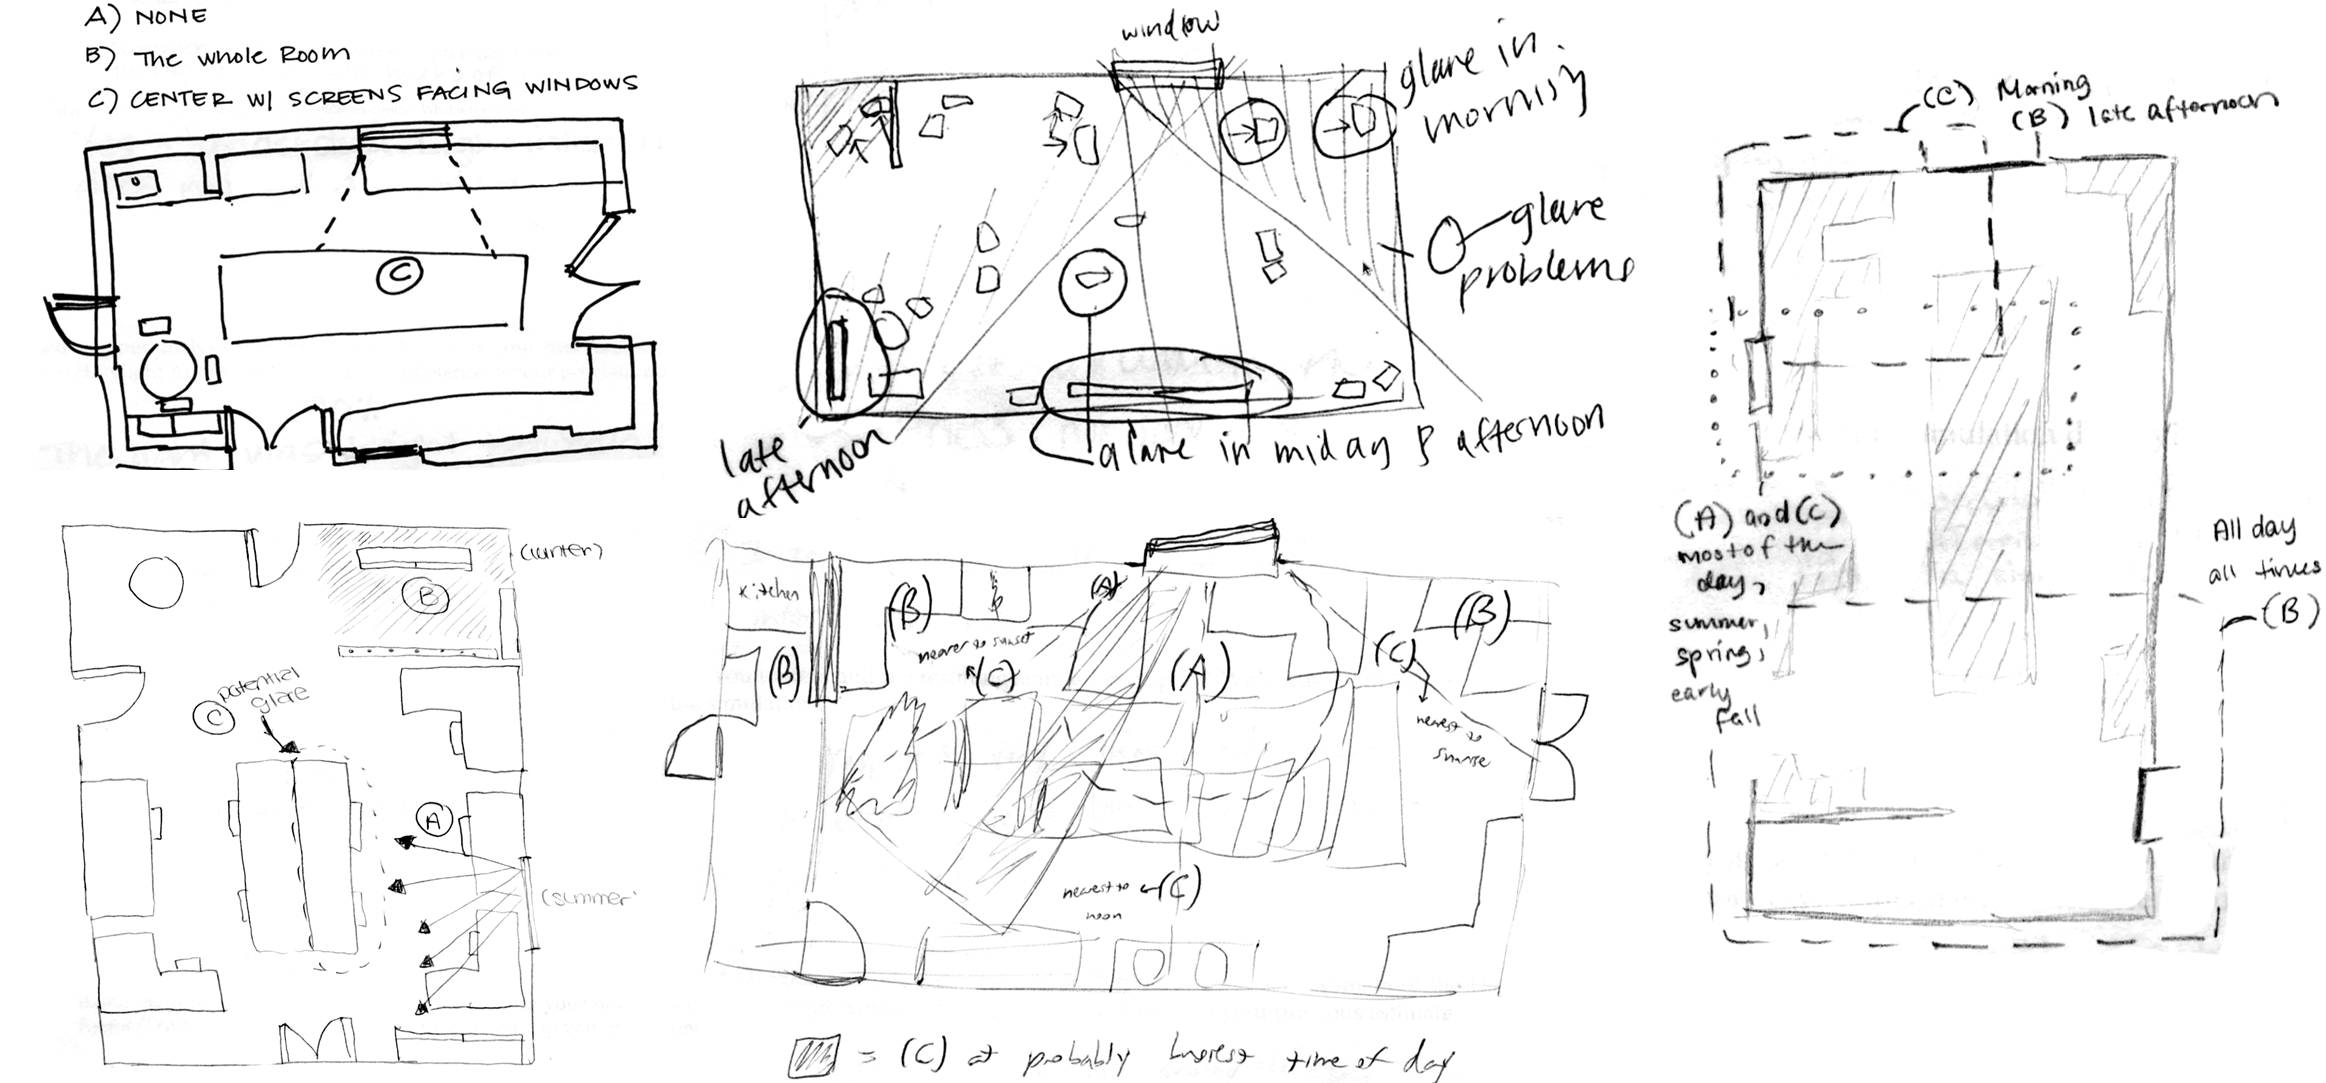
\includegraphics[width=7.0in]{images/sketches/all_together}%
%
\vspace{-2.7in}
{\bf A4} \hspace{1.9in}
{\bf A3}
\vspace{2.3in}
\\
{\bf A5} \hspace{1.8in}
{\bf N2} \hspace{3in}
{\bf N4}
\vspace{-0.1in}\\
%
\caption{In Part 1 of the study, participants were asked to sketch the
  lab room and annotate this sketch with their intuition about areas
  with A) too much daylighting, B) too little daylighting, and C)
  potential for glare.  The sketches demonstrate a variety of detail
  and accuracy in the analysis of the dynamic lighting conditions. }
\label{figure:sketches}
\end{figure*}


As the field of Tangible User Interfaces has advanced, a variety of
design tools have been demonstrated in different application areas.
Lucchi et al. ran a user study comparing design interaction on two
tabletop surfaces with different interaction techniques: tangible
interaction and touch interaction~\cite{1709917}.  In their
comparison, the tangible interface allowed users to perform tasks more
quickly.  This comparison assumed fully functional interfaces for both
systems and not simply the least common denominator of a tangible and
multi-touch interface.  When validating TUIs through user studies,
researchers frame questions appropriately and thoughtfully compare
the results from inherently different interfaces.  Mechanix is a tool
which teaches children about simple machines~\cite{TsengBB11}.  Based
on tracking using a webcam, children could learn how to design simple
mechanical objects and observe how the objects interact.  TUIs provide
a valuable way for children to design and observe while using a simple
interface.  The Luminous-Tangible Workbench~\cite{Urp99urp:a}
provided a tangible interface for urban planning.  It showed the
shadows buildings cast upon one another, but did not simulate lighting
in interior spaces.

Many TUIs are designed to both be an informative tool as well as to
encourage creativity.  The JUMP tool~\cite{1268540} rectifies multiple
architectural documents (e.g., electrical and mechanical) for a
construction project.  The prototype interface involves placing a
different token on the workspace to view each document.  A formal user
study of this tool revealed that often the users felt as if they were
in a foreign environment with these primitives and preferred a more
traditional method of interaction (mouse and keyboard).  Thus, our
ongoing investigations must also compare our novel daylighting
interface to traditional interfaces and existing software and evaluate
the benefits and limitations.  While TUIs as design tools is an
exciting prospect, it is important to ensure that users feel as
comfortable using the new tool as the alternative.


While using TUIs as design tools is an exciting prospect, it is
important to make sure users feel as comfortable using the new tool as
the alternative.  Also, consideration should be made to the efficiency
of using the new tool to traditional interfaces.

%Cut?
%For example, a device for vibrational input with light
%output~\cite{1709908} was demonstrated
%for augmenting musical performances(education).
%tudies in the field have even looked into new input methods for cell
%phones~\cite{1709906}.  Gestures like whacking or wiggling your cell
%phone are proposed as a new way to silence a call or send it to
%voicemail(remove reference).
%TUIs seldom have any traditional interface and as such it is often necessary to look
%at various novel interfaces both for input and for communicating back to the user.  Vibration, touch %and light
%are just a few of the possibilities for input and output to and from interfaces.





%\vspace{-0.05in}
\section{Research Questions}
%\vspace{-0.05in}

The common themes of related work on TUIs, education, accuracy, and
design, also motivated
%the design of our user study.
our study of the architectural daylighting system.


%\vspace{-0.05in}
\subsection{Daylighting Intuition and Education}
%\vspace{-0.05in} 

One key question addressed was: ``How much intuition about daylighting
do people have?''  We believe our system will be useful both for those
who need to expand their daylighting knowledge as well as those with
limited knowledge.  We hypothesize that many users' pre-existing
daylighting understanding may be limited to general knowledge such as
``more sun in the summer'' and ``the sun travels from east to west in
the sky''.  Our system provides more concrete information such as the
exact path of the sunspots traveling across a specific building
geometry, problematic glare locations and times, and the relative
intensities of light as it diffusely reflects different surfaces and
materials throughout the space.  If our study reveals common flaws in
participants' pre-existing daylighting understanding, the tool could
prove beneficial for architectural education.  Another key question
is: ``To what extent can the tool correct deficiencies in the users'
daylighting intuition?''  We hypothesize that users will have a better
overall understanding of daylighting in a variety of spaces after
using the system.  We believe that our system can communicate both
information about how bright a room will be on a given day as well as
when and where glare will be particularly problematic in a scene.

%\vspace{-0.05in}
%\subsection{Education}
%\vspace{-0.05in} 

%One key question addressed was: ``How much intuition about daylighting
%do people have?''  We hope our system will be useful both for those
%who need to expand their daylighting knowledge as well as those with
%limited knowledge.  We hypothesize that many users' pre-existing
%daylighting understanding may be limited to general knowledge such as
%``more sun in the summer'' and ``the sun travels from east to west in
%the sky''.  Our system provides more concrete information such as the
%exact path of the sunspots traveling across the room, specific
%problematic glare locations and times, and the relative intensities of
%light as it diffusely reflects throughout the space.  If our study
%reveals common flaws in participants pre-existing daylighting
%understanding, the tool could prove beneficial for architectural
%education.  Another key question is: ``To what extent can the tool
%correct deficiencies in the users' daylighting intuition?''  We
%hypothesize that users will have a better overall understanding of
%daylighting in a variety of spaces after using the system.  We are
%confident that the system can communicate both information about how
%bright a room will be on a given day as well as when and where glare
%will be particularly problematic in a scene.



%\vspace{-0.05in}
\subsection{Accuracy}
%\vspace{-0.05in}


The accuracy of a daylighting simulation is dependent upon the
precision of the model built by the users.  If the designer is sloppy
in specifying the proportions of the room or windows, the orientation
of the building, or the material properties, the resulting simulation
may over- or under-estimate the daylighting.  When a person visits an
existing space, he generally has a better sense of the dimensions and
proportions of the space.  We ask the question: ``How accurate are
users at modeling with our tool a space they visit and observe?''
Given that daylighting is dependent upon only upon relative
proportions and not absolute size, thus we focus on the relative
dimensions.  The accuracy of a simulation is also dependent upon
attention to detail.  Thus we ask: ``How accurately do users remember
and reproduce details in a space, i.e., interior partitions, window
dimensions, and ceiling height?''  Some details are more important
than others for daylighting analysis and have a more significant
impact on the lighting calculations.  Finally, the accuracy of our TUI
is ultimately dependent upon the display and perception of the
simulation results.  ``Do the users accurately perceive and interpret
the displayed information?''  We investigate both the accuracy of
proportions and attention to details in this study.  We also study the
users' response and interpretation of the daylighting visualization.


%The accuracy of a lighting simulation is dependent upon the precision
%of the model built by the users.  If the designer is sloppy in
%specifying the proportions of the room or windows, the orientation of
%the building, or the material properties, the resulting simulation
%will over- or under-estimate the daylighting.  When a person visits an
%existing space, he generally has a better sense of the dimensions and
%proportions of the space.  We ask the question: ``How accurate are
%users at modeling a space they can visit and observe?''  Given that
%daylighting is dependent upon relative proportions and not absolute
%size we can focus on the relative dimensions.  The accuracy of the a
%simulation is also dependent upon attention to detail.  ``How
%accurately do users remember and reproduce details in a space, i.e.,
%interior partitions, window dimensions, and ceiling height?''  Some
%details are more important than others and have a more significant
%impact on the lighting calculations.  Finally, the accuracy of the
%tool is ultimately dependent upon the display of the simulation
%results.  ``Do the users accurately perceive and interpret the
%displayed information?''  We will investigate both the accuracy of
%proportions and attention to details in this study.  We will also
%study the users' response and interpretation of the daylighting
%visualization.

 %People are generally more accurate in spaces they have been in.  %\fbox{move later} By using an existing space and having people sketch and evaluate it, the users accuracy can be quantitatively measured.  Evaluating the predictions of users enabled us to gain a better understanding of their intuition regarding daylighting: whether peoples knowledge of daylighting was uniform across people in the program or whether it varied more and seemed to have been acquired elsewhere.  

%Accuracy can be measure both by the ratio of lengths of components in the room such as walls and windows as well as comparing users' attention to details; some users including interior walls (in the form of partitions) while others did not take this into account.

%The study also investigates whether users have a firm grasp on what times and days are useful to look at in daylighting analysis.  If users know that it is important to study the extremes of possible lighting conditions, then we would know that they could, given a satisfactory tool, analyze daylighting well.  If users did not possess this knowledge, we would know that training on the sun's position in relation to the seasons would also be useful.

%Finally, we are interested in how accurately users perceive the light shown in the space.  If we photo-realistically reproduce a scaled model of lighting and yet users cannot perceive the change, then this must be remedied by communicating information in a different manner.

%accuracy of proportions
%attention to details



\begin{figure*}[t]
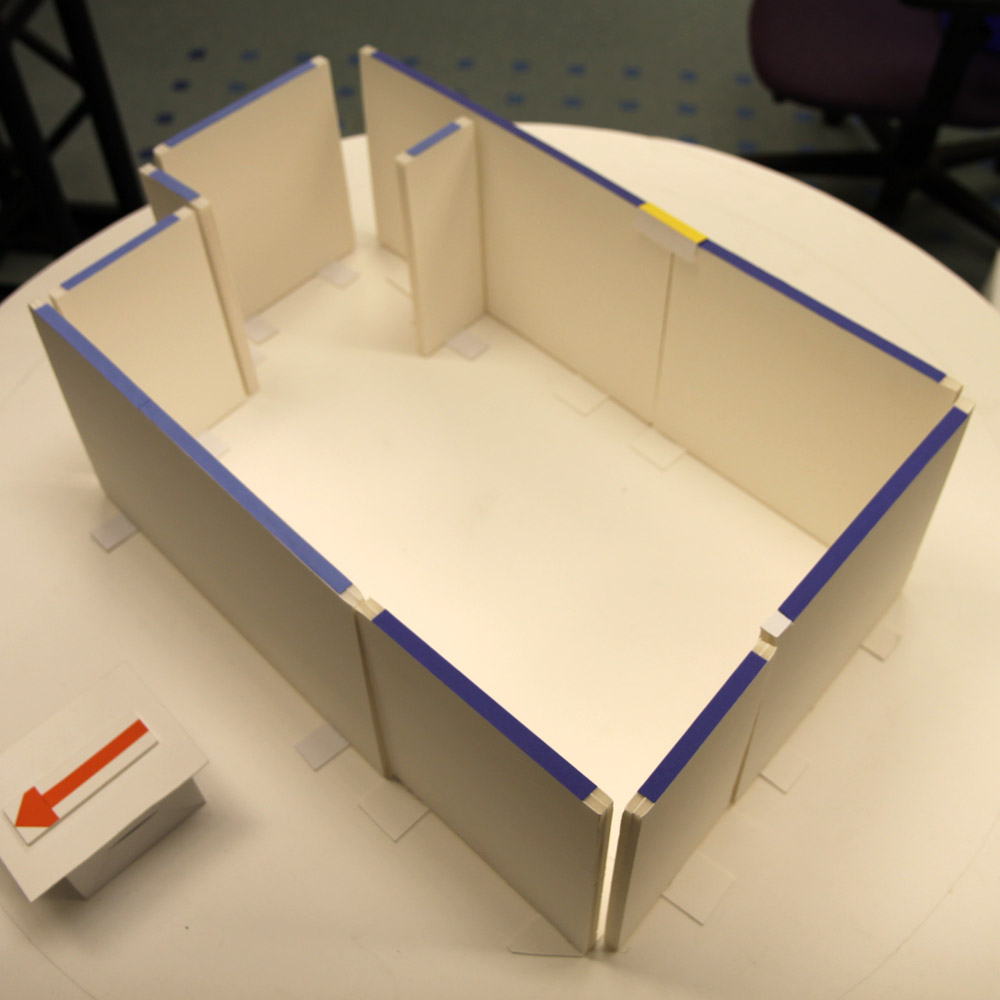
\includegraphics[width=1.9in]{images/photos/63_original} %N1
\begin{minipage}[b]{4.9in}
  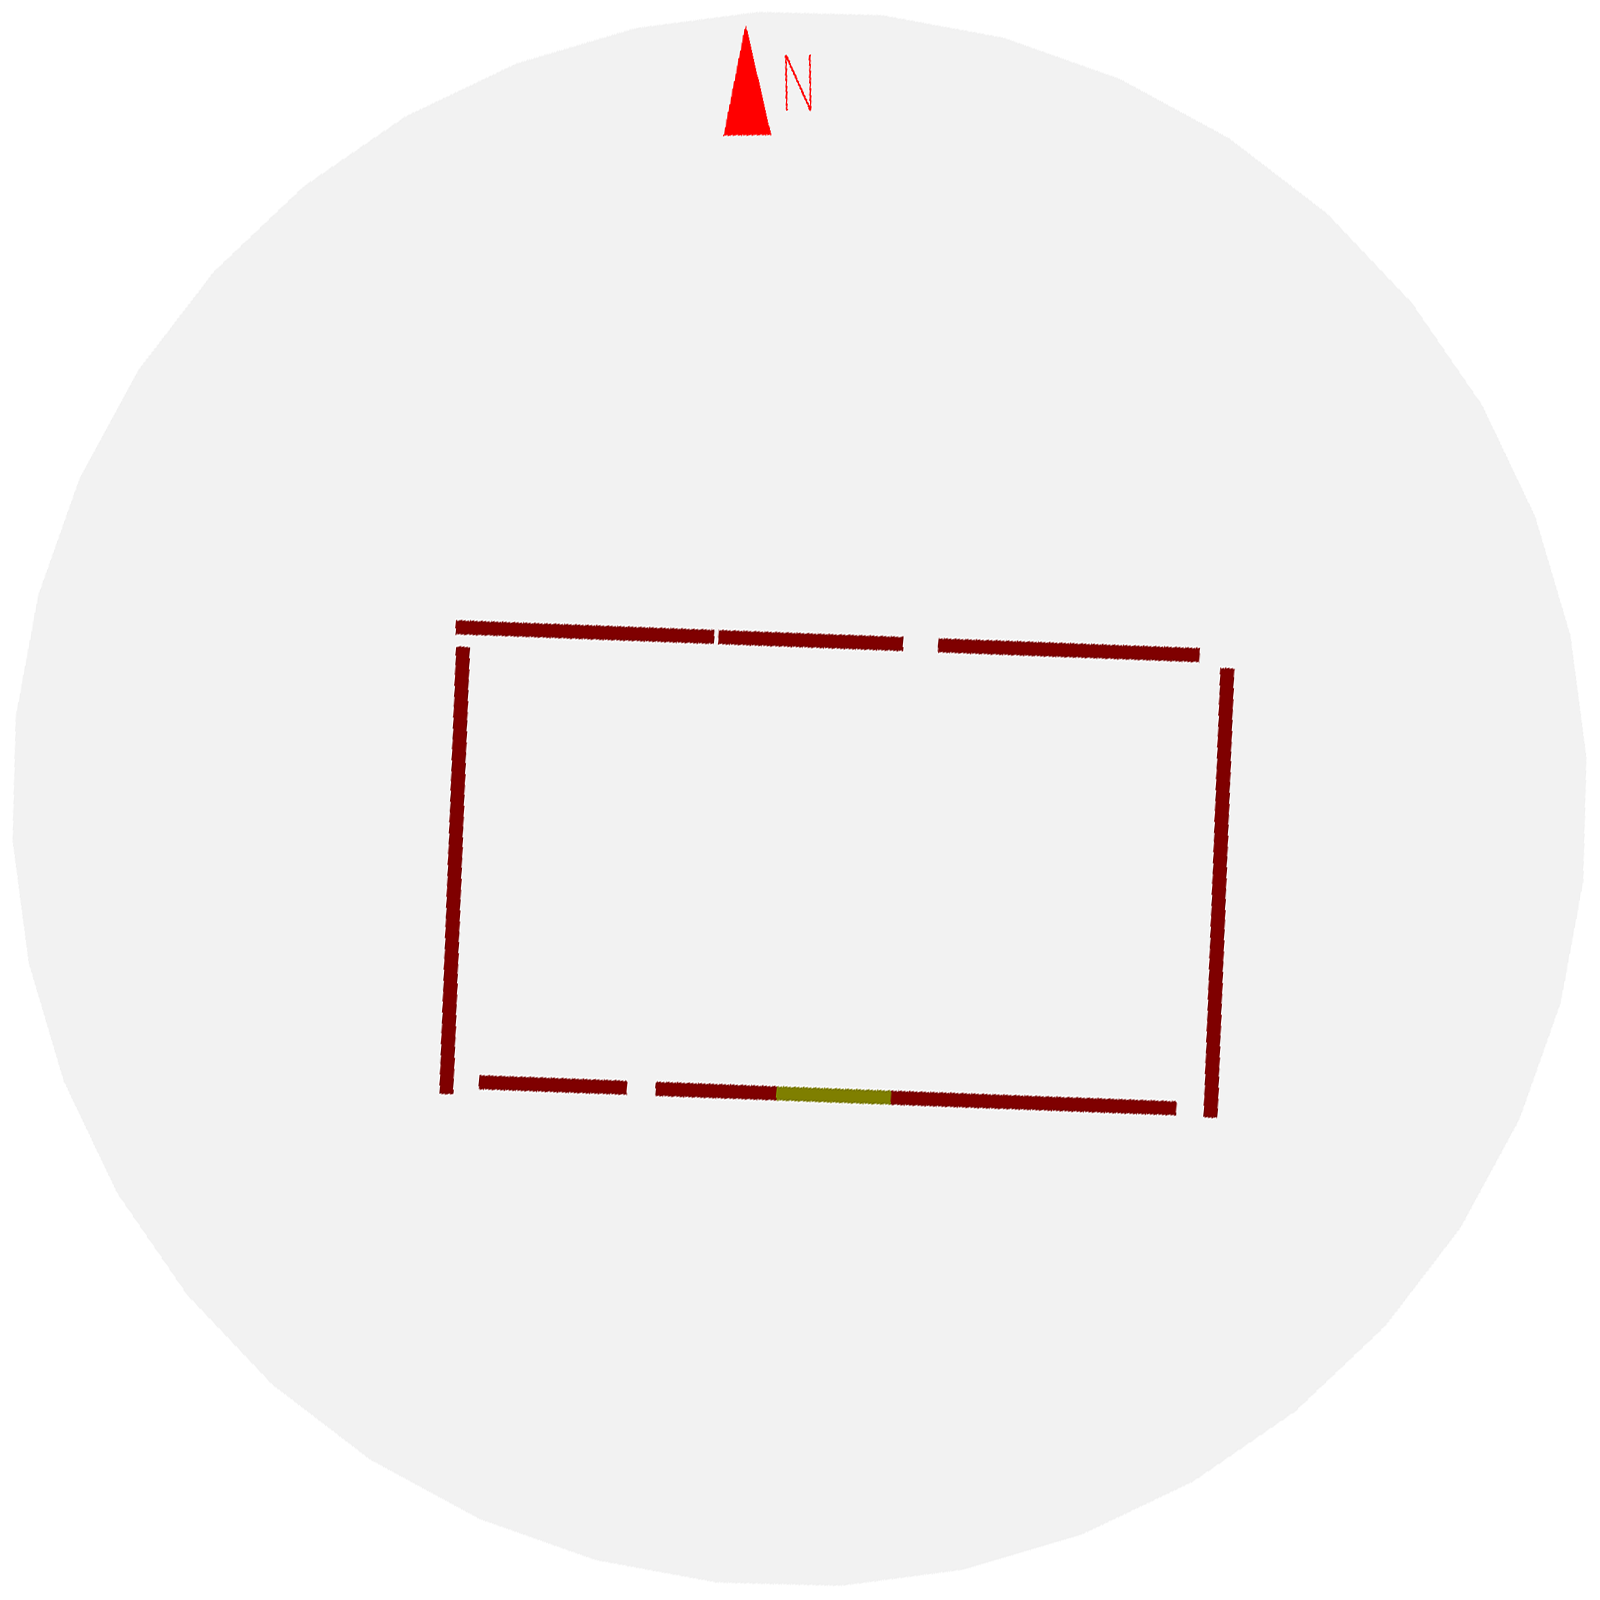
\includegraphics[width=0.95in]{images/section2/0_2D_walls_rotate} %A1
  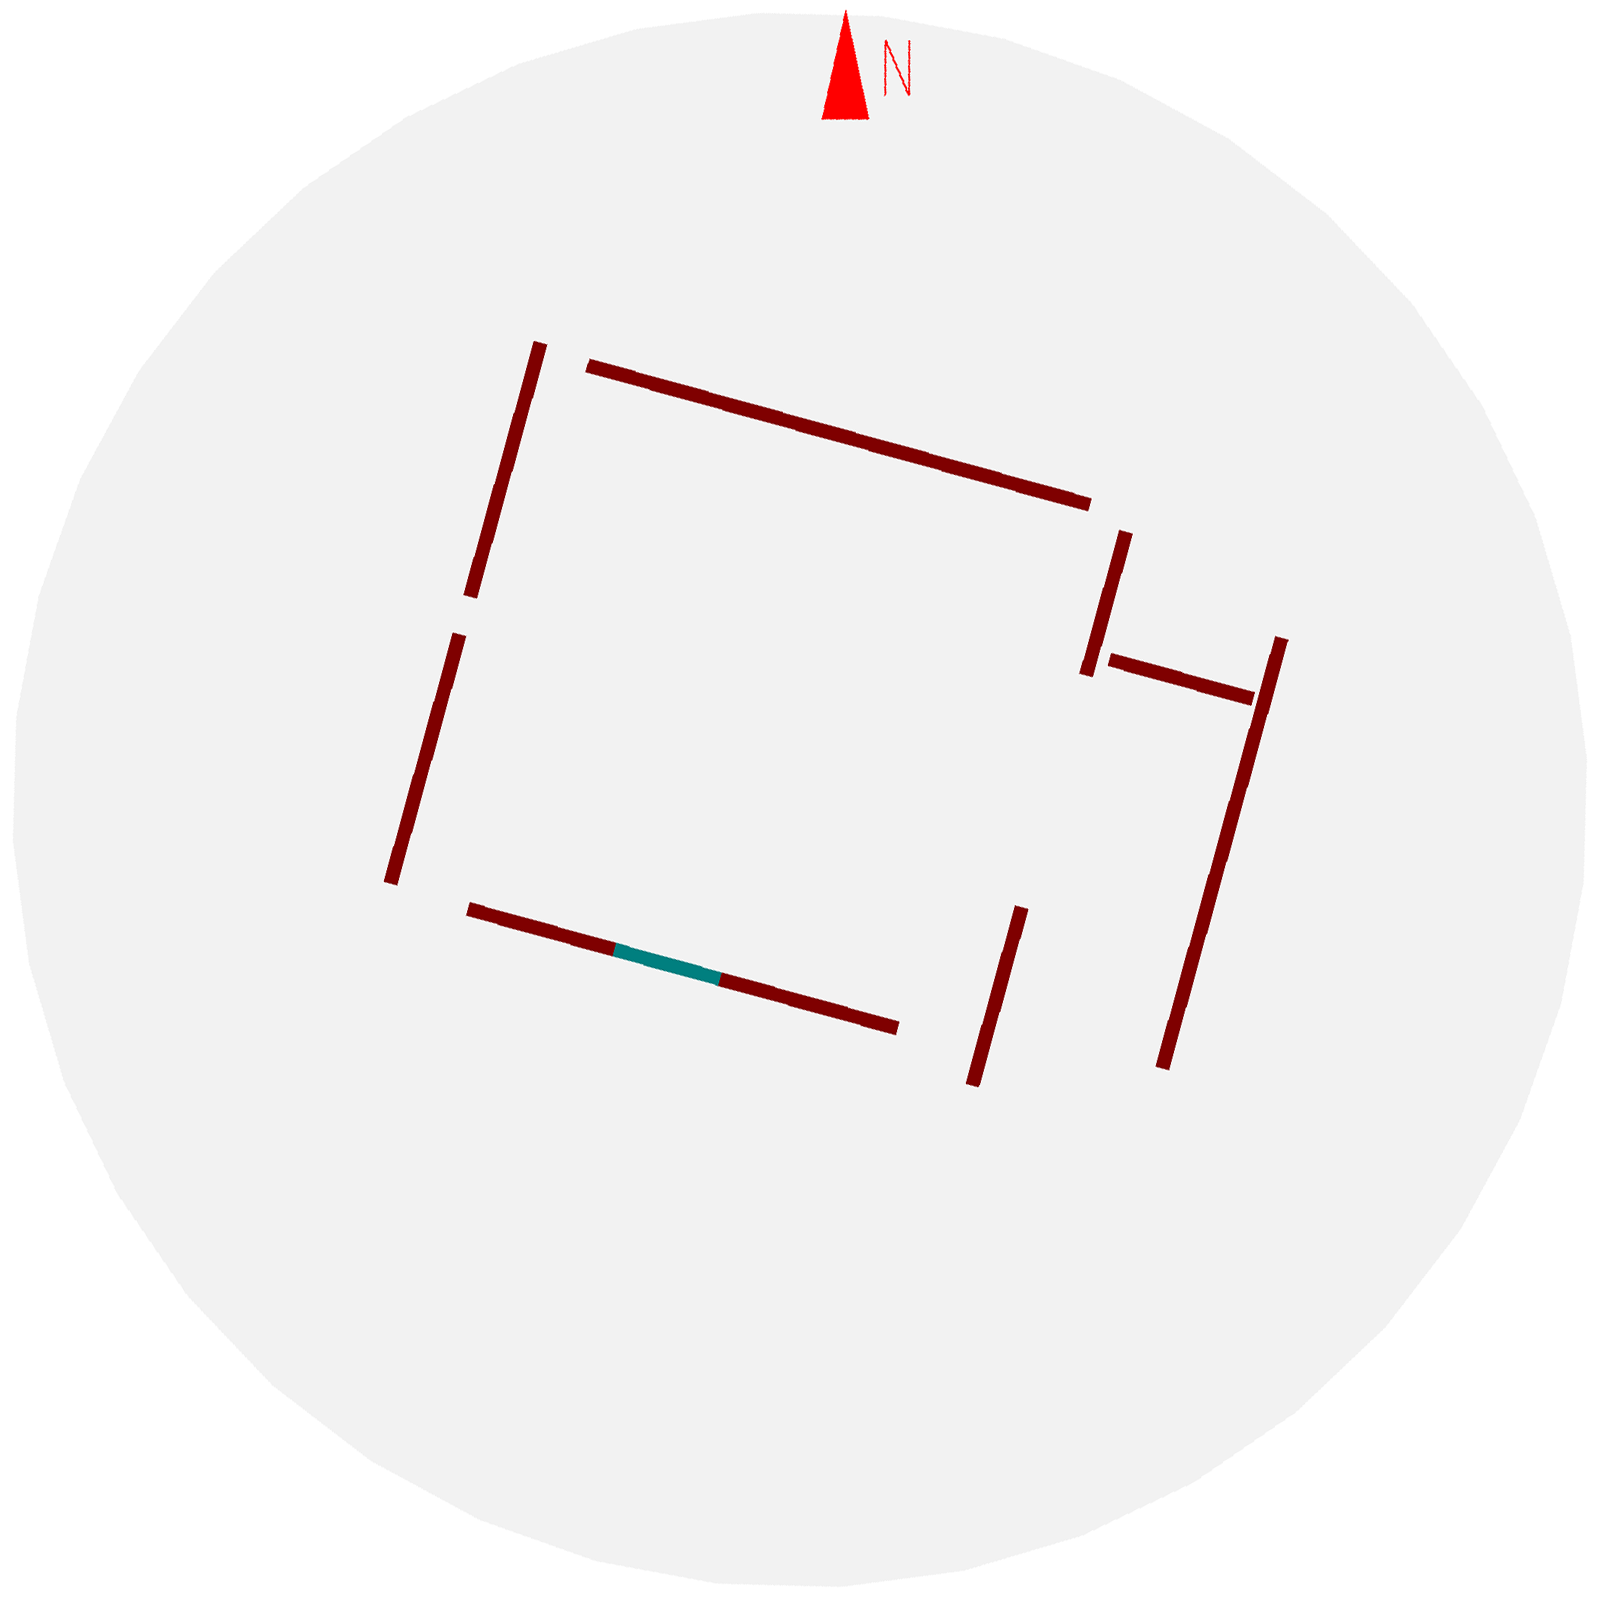
\includegraphics[width=0.95in]{images/section2/2_2D_walls_rotate} %A2
  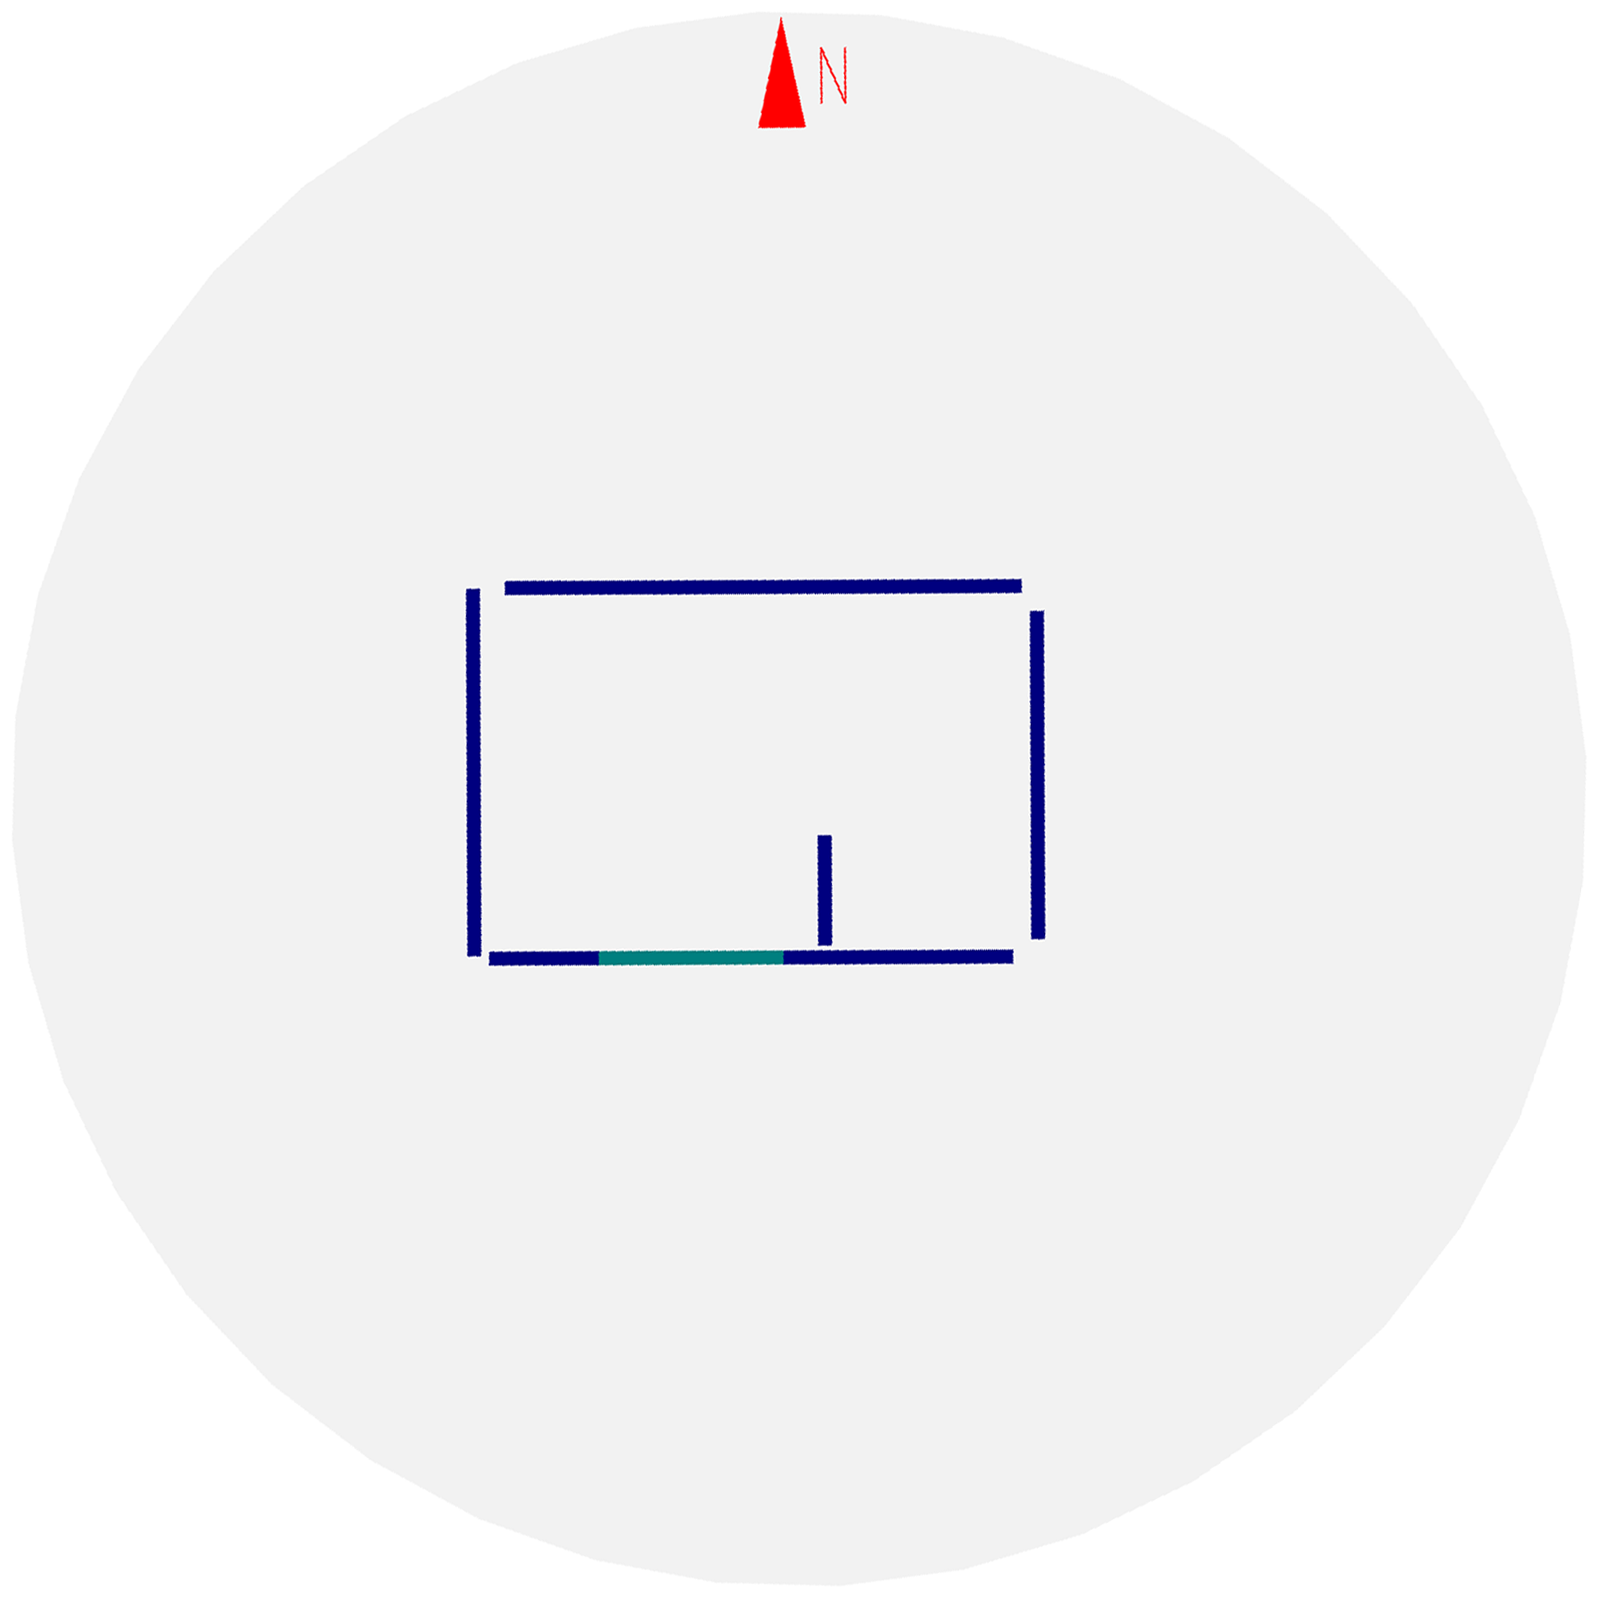
\includegraphics[width=0.95in]{images/section2/6_2D_walls_rotate}  %A4
  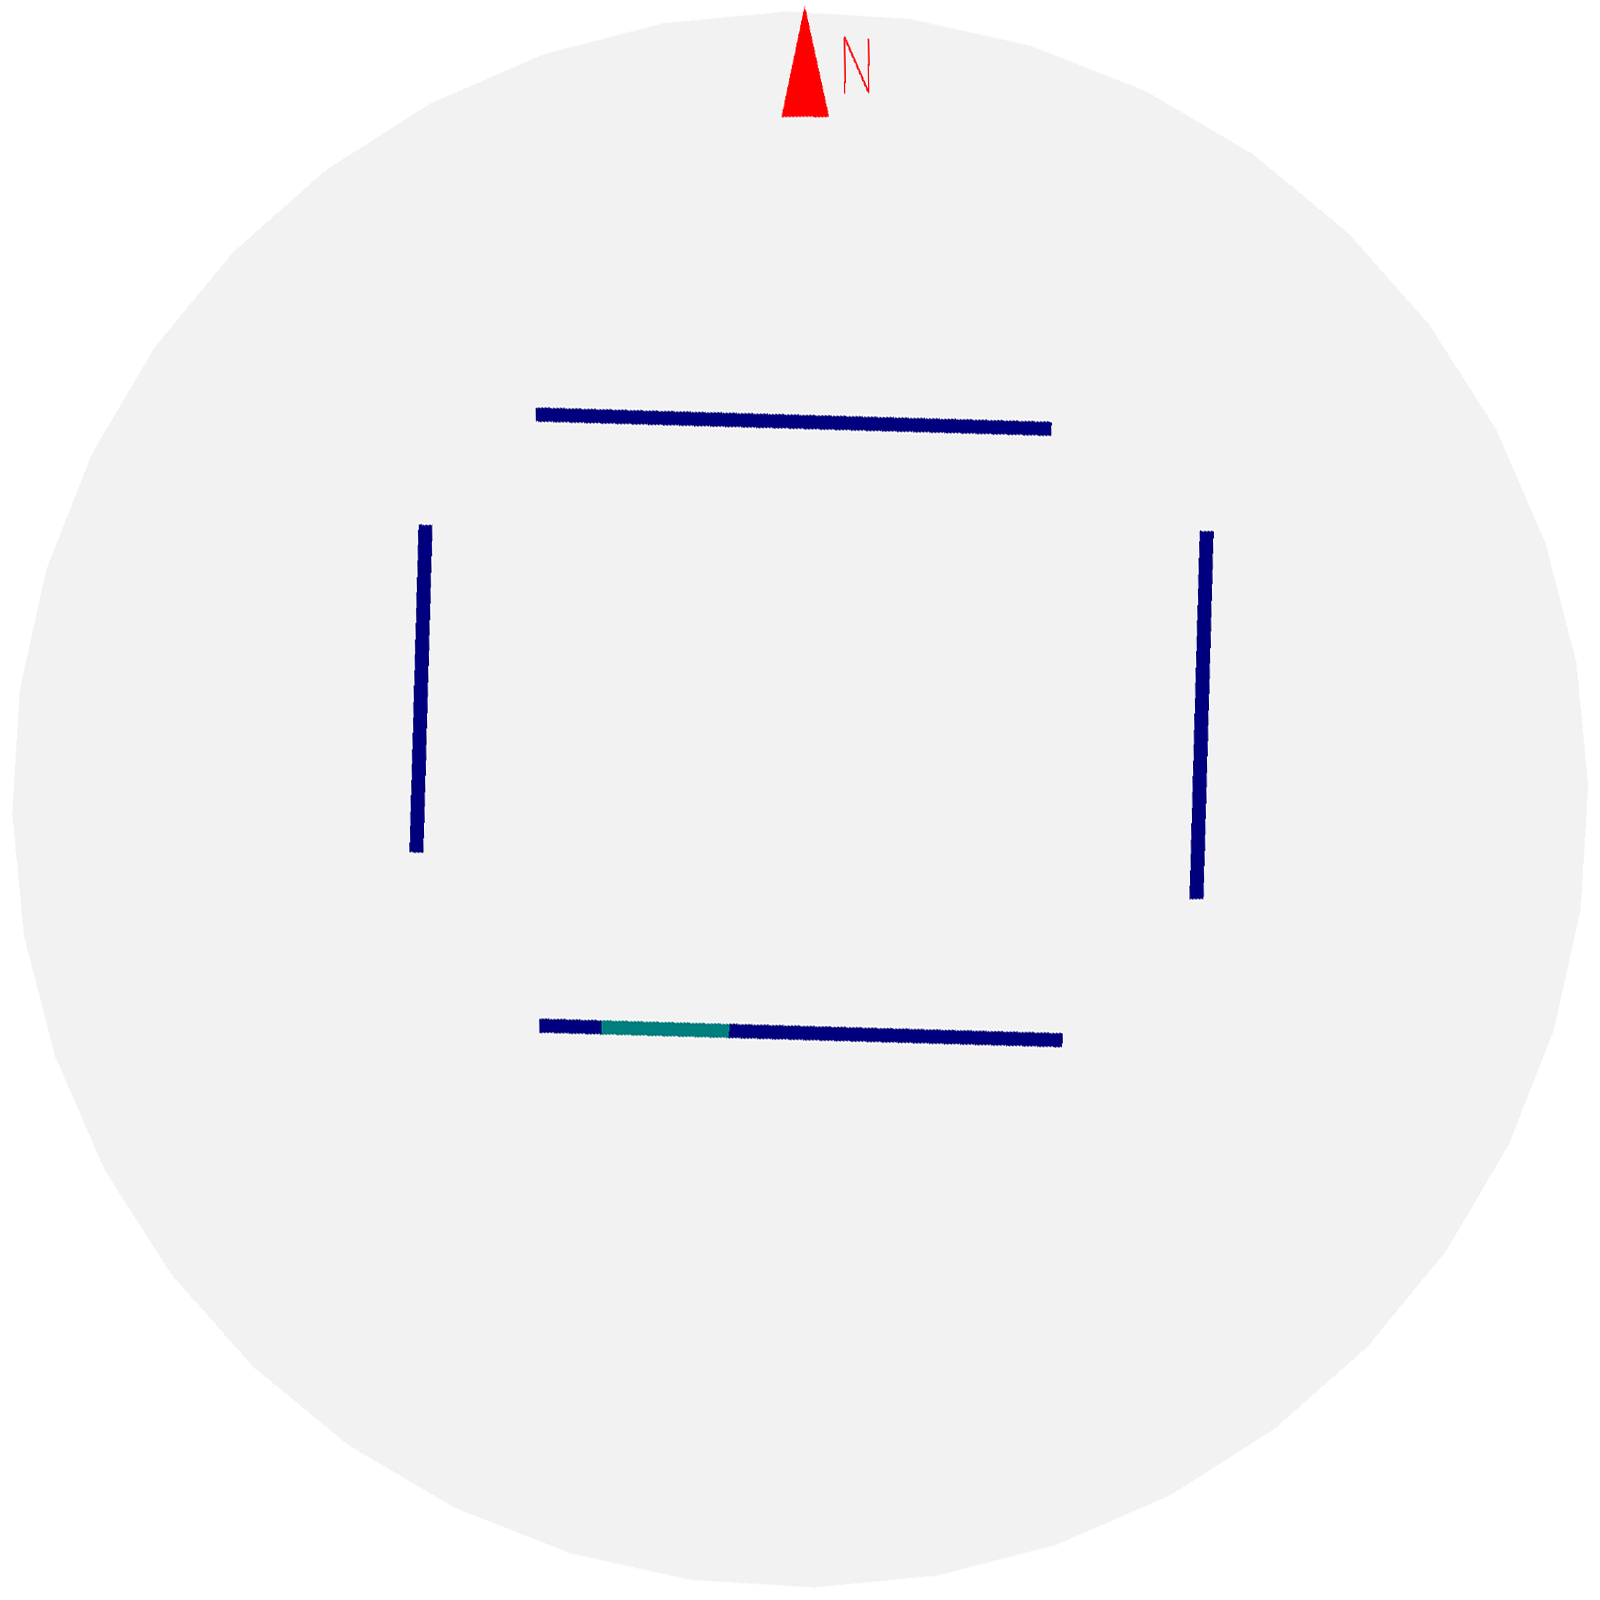
\includegraphics[width=0.95in]{images/section2/7_2D_walls_rotate} %A5
  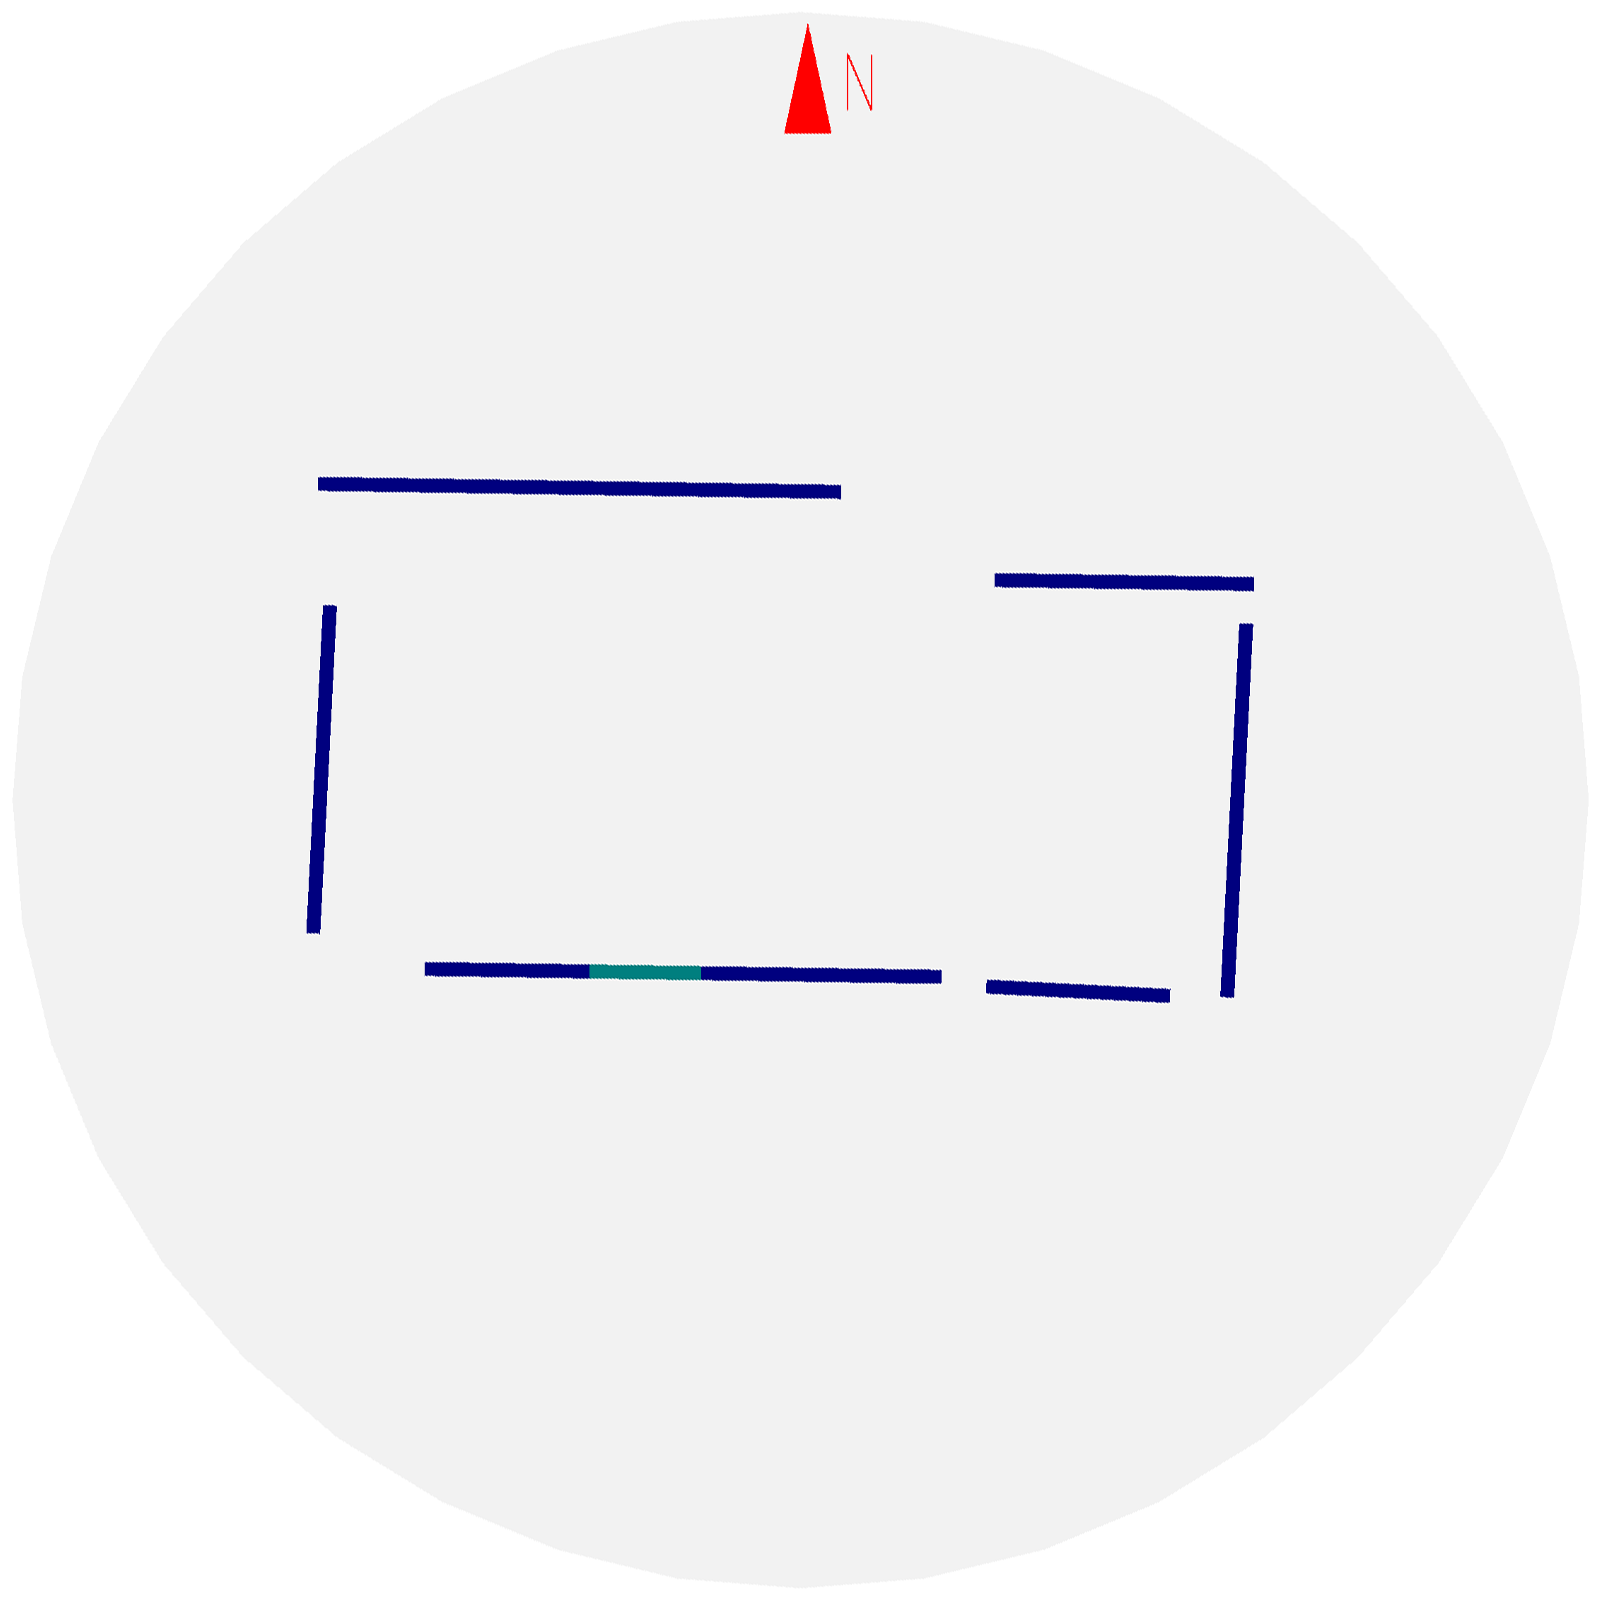
\includegraphics[width=0.95in]{images/section2/8_2D_walls_rotate}\\ %A6
  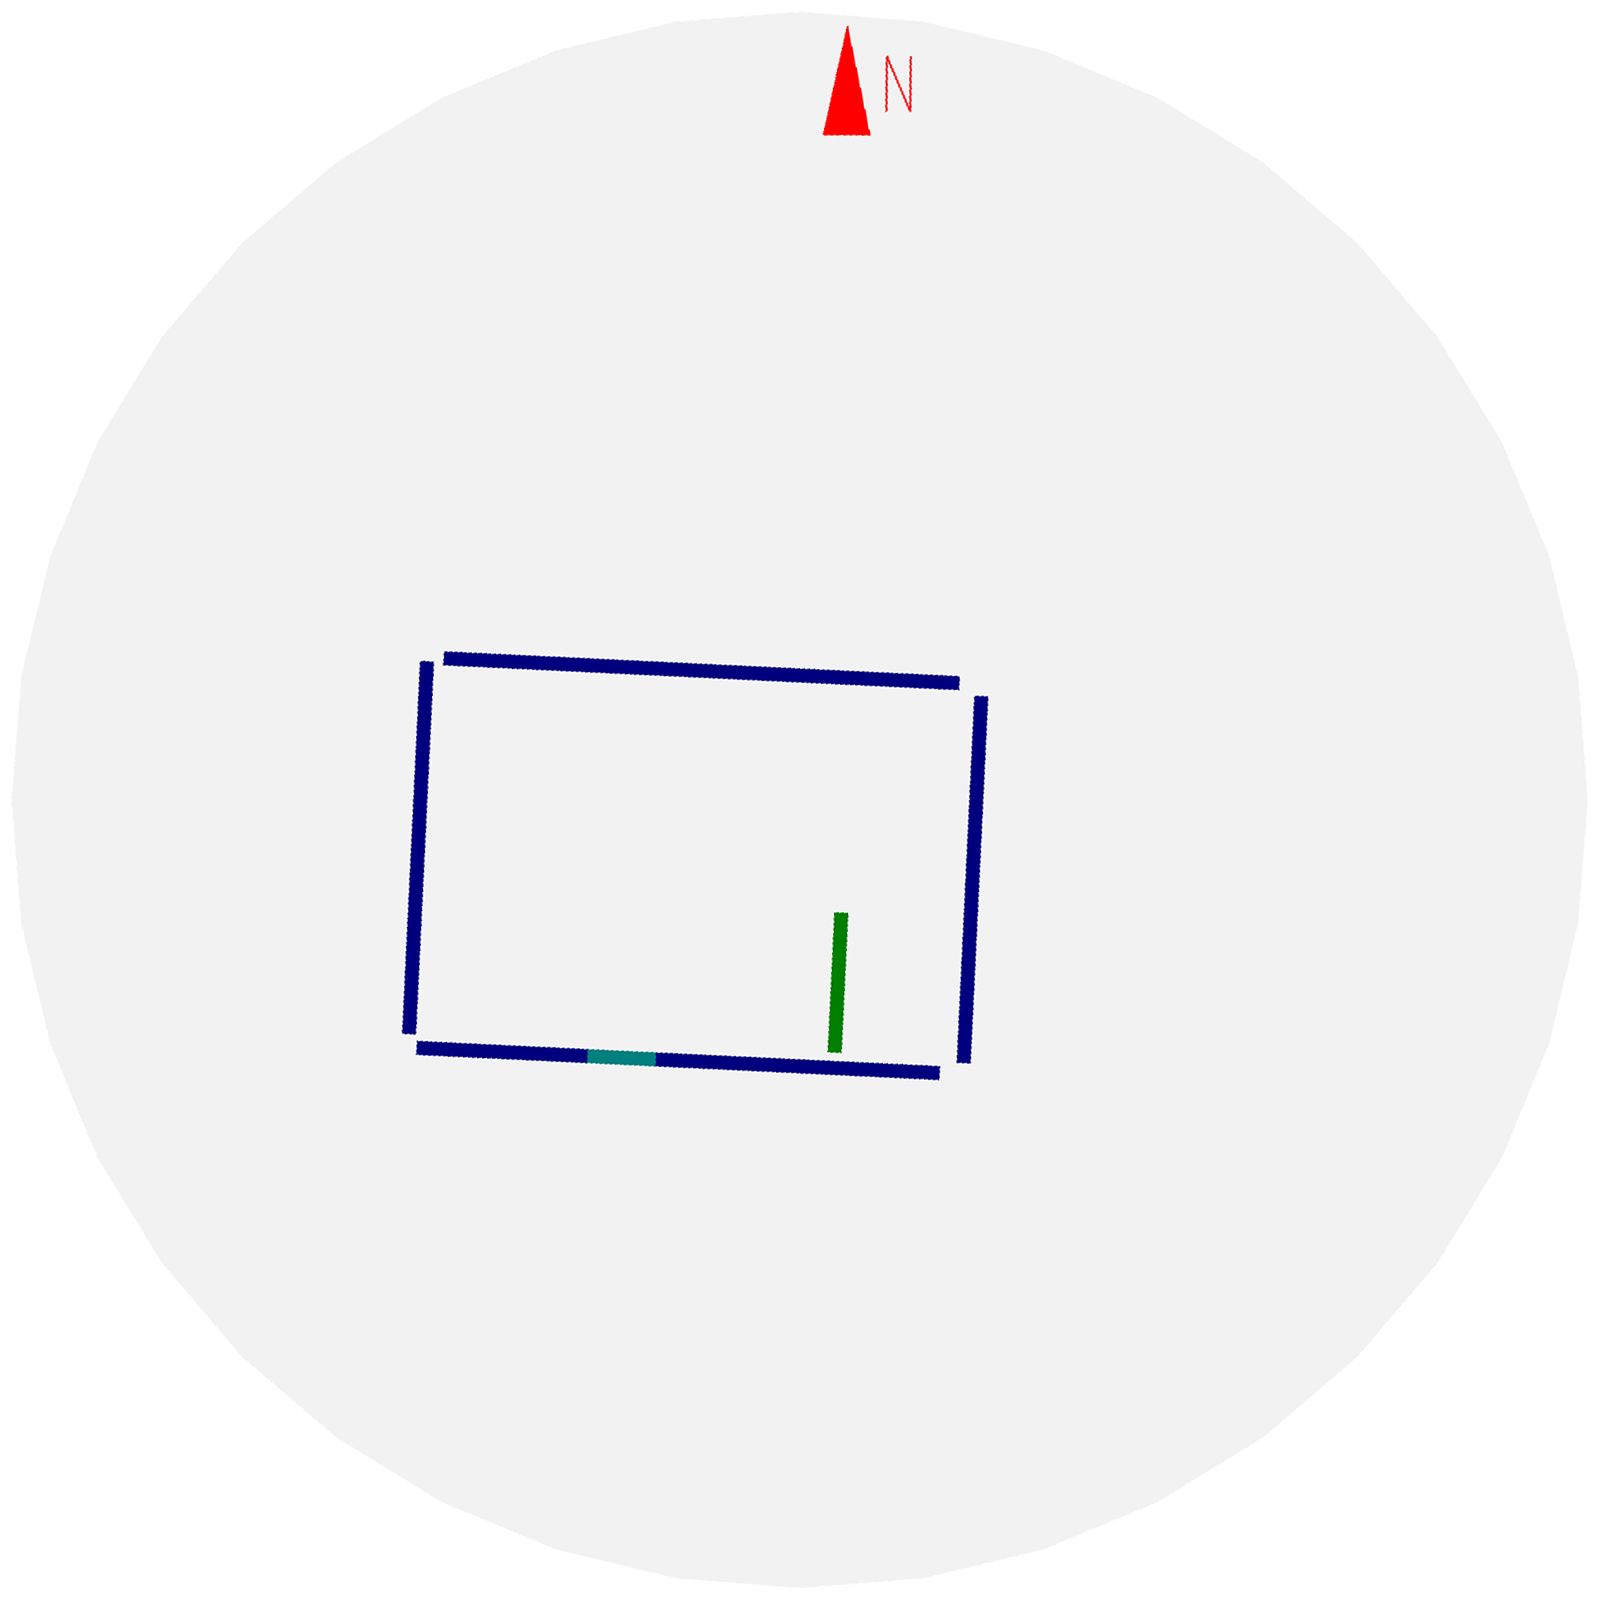
\includegraphics[width=0.95in]{images/section2/3_2D_walls_rotate} %N2
  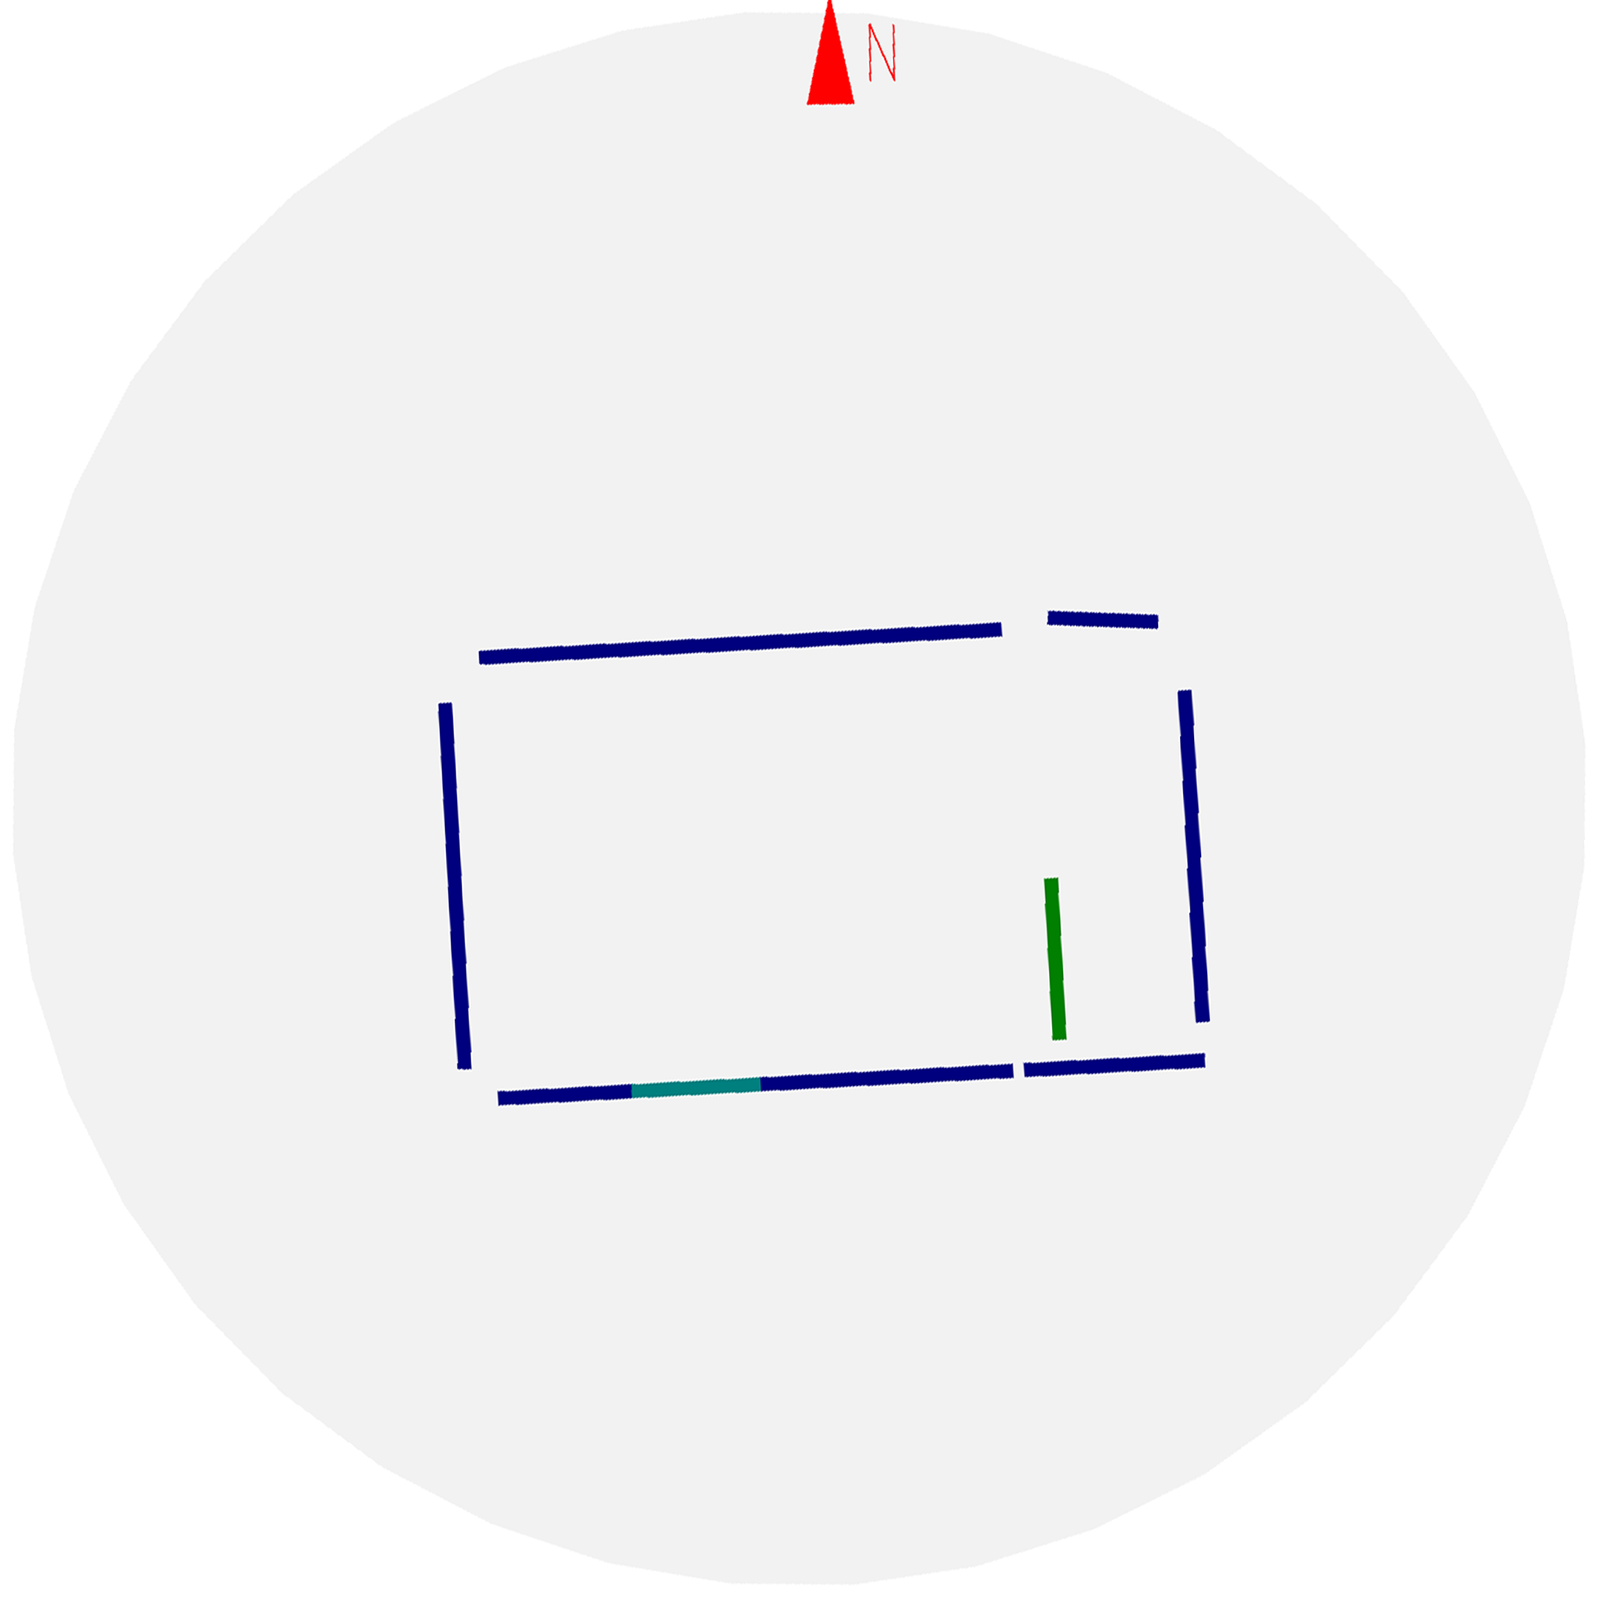
\includegraphics[width=0.95in]{images/section2/5_2D_walls_rotate} %N4
  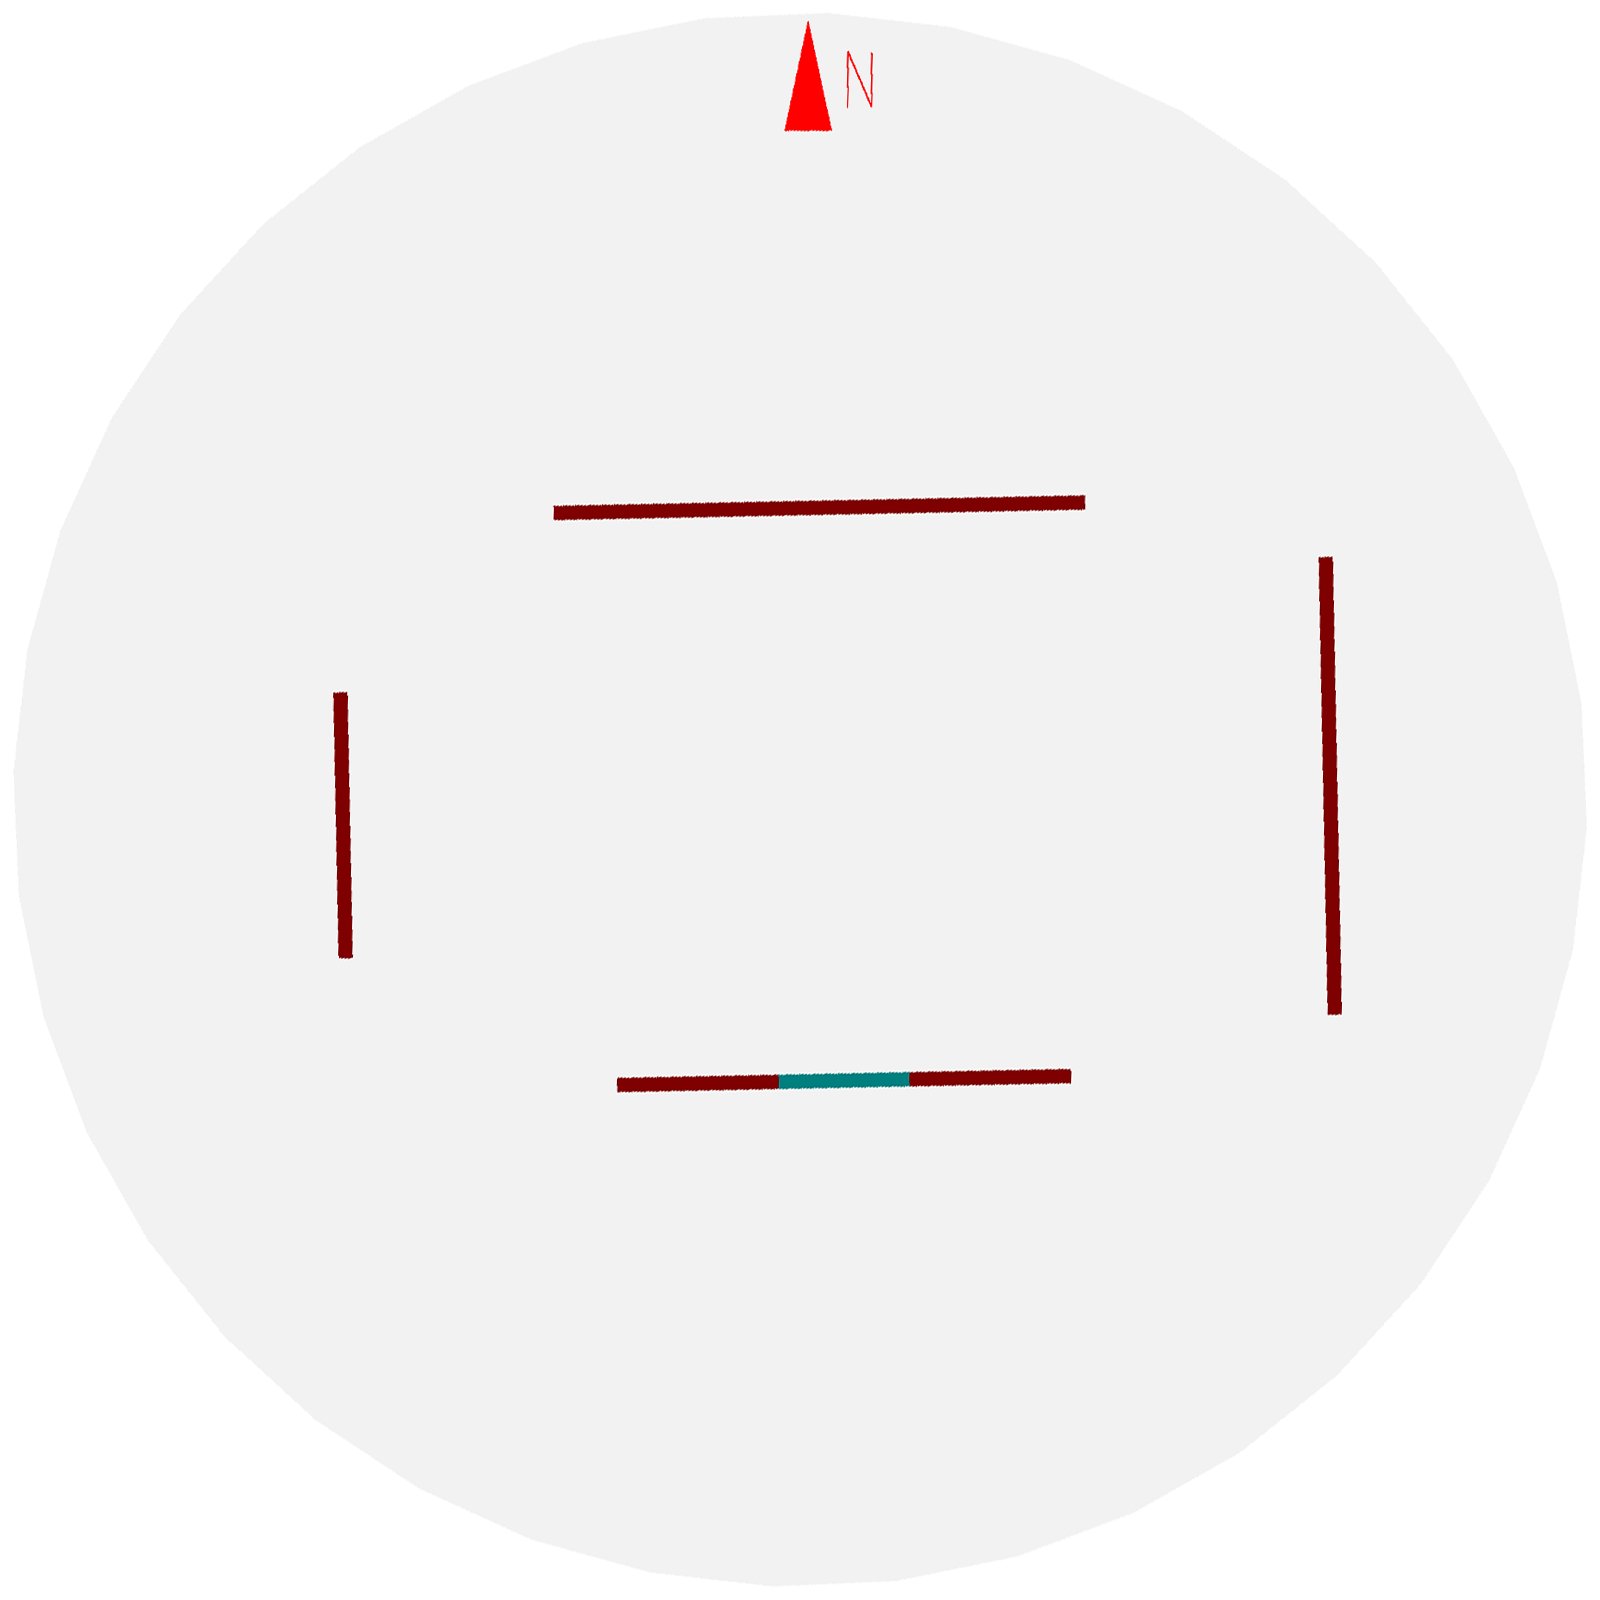
\includegraphics[width=0.95in]{images/section2/9_2D_walls_rotate} %N5
  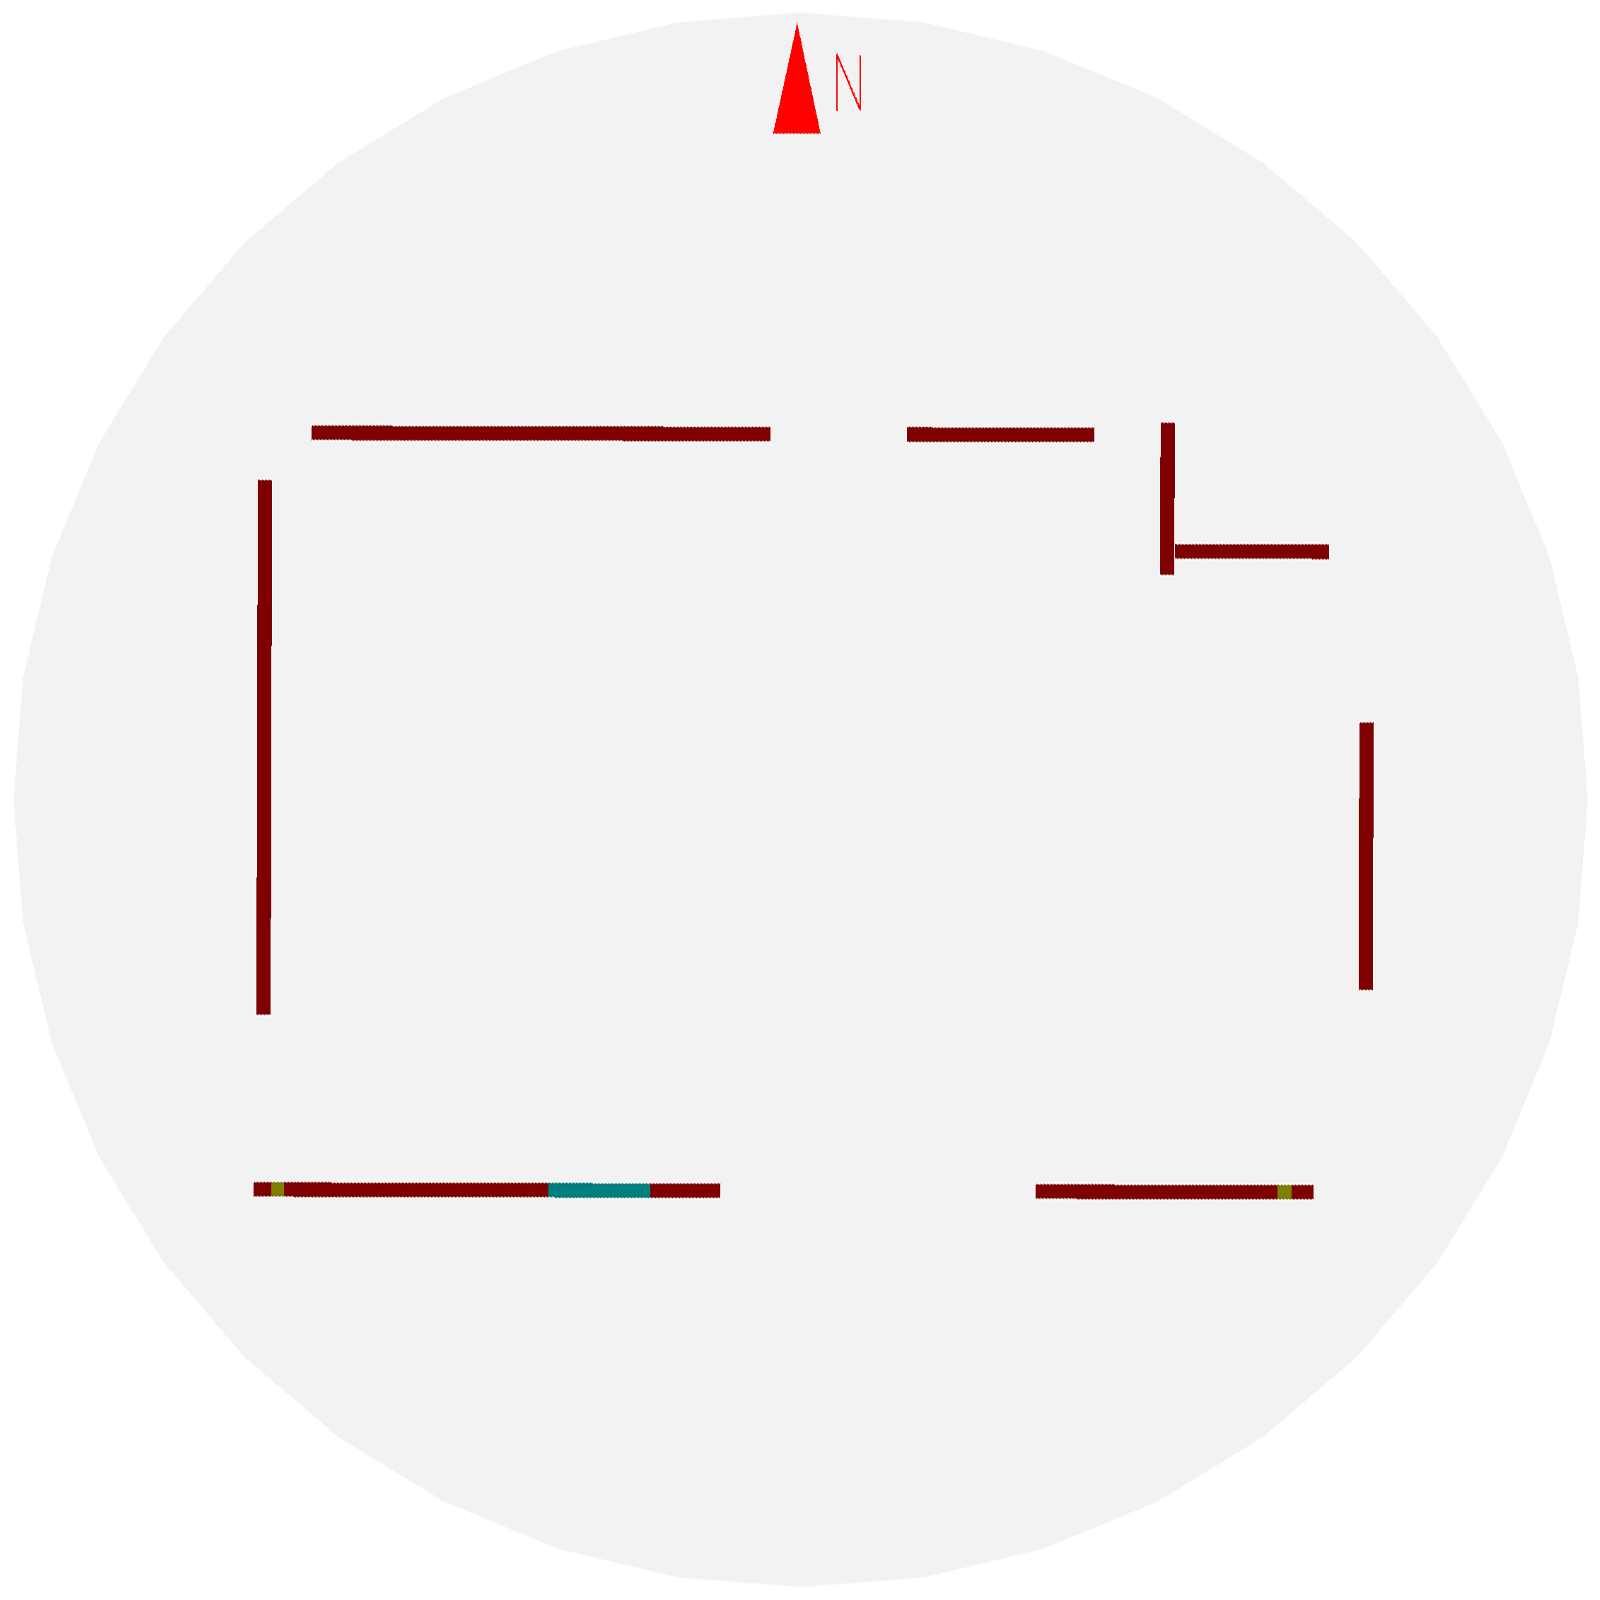
\includegraphics[width=0.95in]{images/section2/10_2D_walls_rotate} %N6
  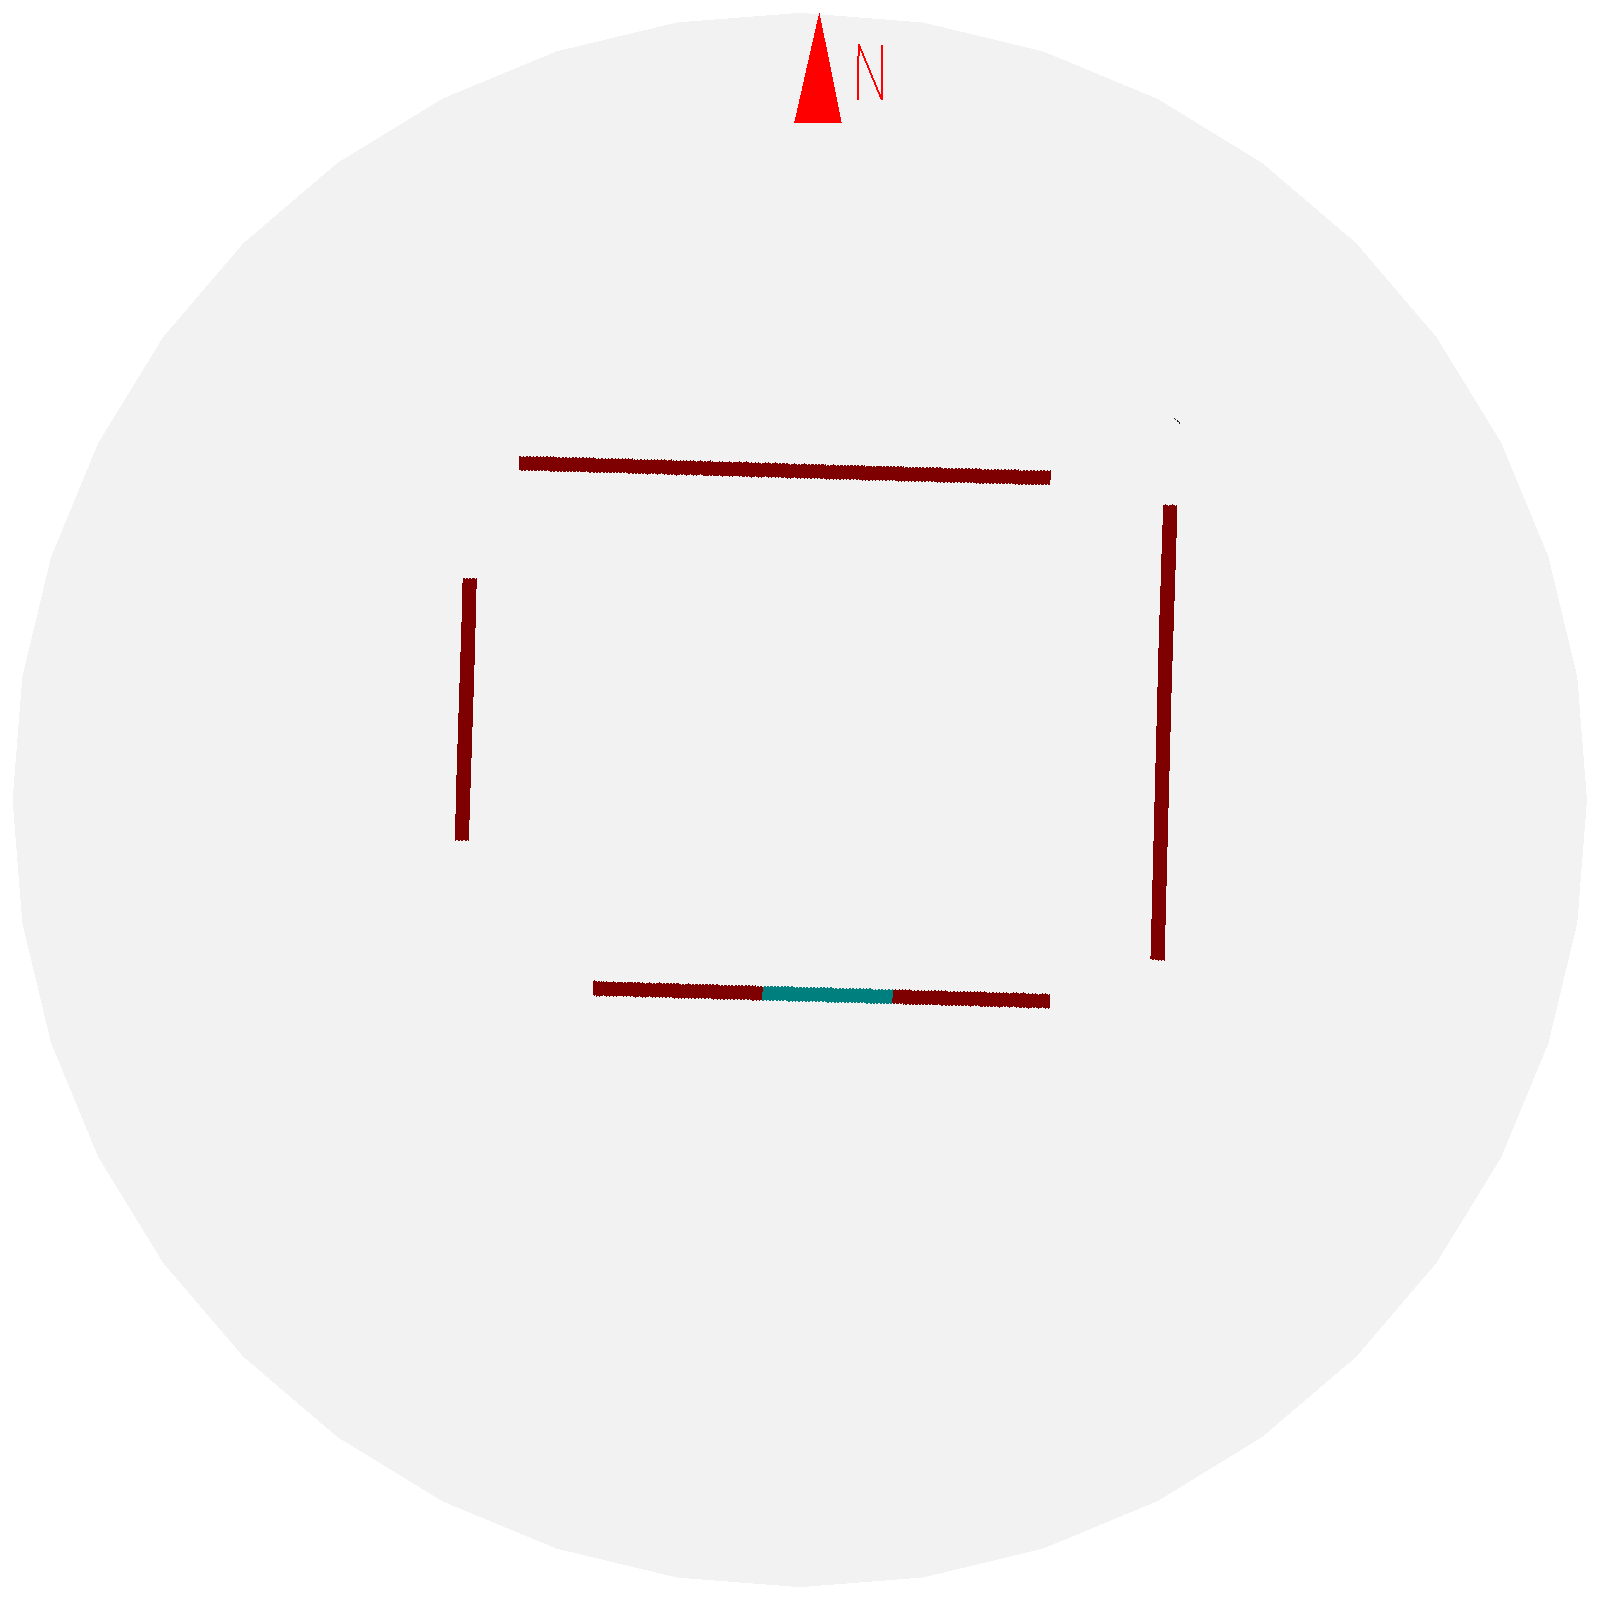
\includegraphics[width=0.95in]{images/section2/11_2D_walls_rotate} %N7
\end{minipage}
\vspace{-1.12in}
\\
\begin{minipage}{1.92in}~\end{minipage}
\begin{minipage}{0.95in}{\bf A1}\end{minipage}
\begin{minipage}{0.95in}{\bf A2}\end{minipage}
\begin{minipage}{0.95in}{\bf A4}\end{minipage}
\begin{minipage}{0.95in}{\bf A5}\end{minipage}
\begin{minipage}{0.95in}{\bf A6}\end{minipage}
\vspace{0.78in}
\\
\begin{minipage}{1.92in}{\bf ~N1}\end{minipage}
\begin{minipage}{0.95in}{\bf N2}\end{minipage}
\begin{minipage}{0.95in}{\bf N4}\end{minipage}
\begin{minipage}{0.95in}{\bf N5}\end{minipage}
\begin{minipage}{0.95in}{\bf N6}\end{minipage}
\begin{minipage}{0.95in}{\bf N7}\end{minipage}\vspace{-0.0in}%\\
  \caption{
  \label{figure:original_designs}
A photograph of the physical geometry of the original office space
constructed by one of the participants for Part 2 of the study and 2D
diagrams of the geometry constructed by the other participants.  Note
the variety of model complexity and scale that users create to
represent the same space.  The red walls are 10 inches tall and the
blue walls are 8 inches tall.  Global illumination renderings of these
geometries are shown in
Figure~\ref{figure:renderingsOfOriginalGeometry}.
}
\end{figure*}



%\vspace{-0.05in}
\subsection{Design}
%\vspace{-0.05in}

A fundamental question of our evaluation is: ``Is this tangible tool
useful in the architectural design process?''  From previous studies,
we believe that users can effectively and creatively design using this
tool.  We predict that users will appreciate the simplicity of the
model construction and speedy production and display of simulation
results.  Furthermore, we predict that when users are presented with
this more complete and detailed representation of daylighting, they
will embrace the benefits of using such a tool regularly, and
potentially incorporate and change how they plan for daylighting use
in their designs.  We also wish to investigate if users feel creative
freedom within the tool.  ``Is users' creativity catalyzed by using
the tool?''  ``Do users feel particular constraints in design because
of the tool?''  We investigate both the advantages and constraints of
using this tool in the design process.


%\vspace{-0.05in}
\section{User Study Design and Protocol}
%\vspace{-0.05in}

Our TUI for daylighting analysis and design is targeted to
professional architects, architecture students, and may be beneficial
for clients and other design fields as well.  Because our tool does
not require much training to use, we claim it is a valuable general
educational tool for daylighting.  In order to answer the questions
outlined in the previous section, we recruited a pool of thirteen
current university students.  Six of the users were architecture
students (labeled A1-A6), all with at least two years of architecture
education and seven students from other departments (labeled N1-N7),
but many with a background in electronic media, arts, and
communication (5 students) or games studies (1 student).


%Our daylighting design tool is targeted for architects, architecture
%students, and may be beneficial for clients and other design fields as
%well.  Because our tool does not require much training to use, we
%claim it may be a valuable general educational tool for daylighting.
%In order to answer the questions outlined in the previous section, we
%recruited a pool of 13 current university students.  Six of the users
%were architecture students (labeled A1-A6), all with at least 2 years
%of architecture education and seven students were from other
%departments (labeled N1-N7), but many with a background in electronic
%media, arts, and communication (5 students) or games studies (1
%student).



\begin{table}[b]
\vspace{-0.1in}
\begin{center}
\begin{small}
\begin{tabular}{@{}l@{~~}|@{~~}r@{~~~}r@{~~~}r@{~~~}r@{~~~}r@{~~}|@{~~}c@{~~~}c@{~~~}c@{~~~}c@{}} 
~       &  short   & long     & window  & window  &  wall      &  & & & \\
~       &  wall    & wall     & width   & placement &  height  &  \multicolumn{4}{c}{measurement ratios} \\ 
%How to fit window placement from southwest corner?
~       &  (s)     &  (l)     & (w)     & (p)     &  (h)  &  s:l  &  w:l  &  p:l & s:h \\ \hline
actual  &  24'     &  34'     &  4'     &  10'    &   12'   &\hl{0.71} &\hl{0.12} &\hl{0.29} &\hl{2.00} \\ 
\hline
A1      &  12.0''  &  21.2''  &  3.2''  &  8.8''  &   10''  &  0.57    &  0.15    &  0.41  &  1.20 \\ 
A2      &  14.8''  &  21.2''  &  2.8''  &  6.5''  &   10''  &  0.70    &  0.13    &  0.30  &  1.48 \\ 
A4      &  10.2''  &  15.2''  &  5.1''  &  3.2''  &    8''  &  0.67    &  0.33    &  0.21  &  1.27 \\ 
A5      &  16.2''  &  21.2''  &  3.7''  &  5.5''  &    8''  &  0.76    &  0.17    &  0.26  &  2.02 \\ 
A6      &  12.9''  &  24.5''  &  2.8''  &  7.8''  &    8''  &  0.53    &  0.11    &  0.32  &  1.62 \\ 
N1      &  16.6''  &  23.5''  &  1.8''  &  7.4''  &    8''  &  0.71    &  0.08    &  0.31  &  2.08 \\ 
N2      &  10.2''  &  14.8''  &  1.8''  &  5.1''  &    8''  &  0.69    &  0.13    &  0.34  &  1.27 \\ 
N3      &  12.0''  &  15.7''  &  3.2''  &  5.5''  &    8''  &  0.76    &  0.21    &  0.35  &  1.50 \\ 
N4      &  12.0''  &  19.8''  &  3.2''  &  3.7''  &    8''  &  0.60    &  0.16    &  0.19  &  1.50 \\ 
N5      &  15.7''  &  26.3''  &  3.2''  & 11.5''  &   10''  &  0.60    &  0.12    &  0.44  &  1.57 \\ 
N6      &  20.3''  &  29.5''  &  3.2''  &  7.8''  &   10''  &  0.69    &  0.11    &  0.27  &  2.03 \\ 
N7      &  13.8''  &  18.5''  &  3.2''  &  8.3''  &   10''  &  0.75    &  0.18    &  0.45  &  1.38 \\ \hline  
averages &          &          &         &         &         &          &          &        &\\
architecture & 13.2'' & 20.6'' & 3.5''  &  6.4''  &   8.8'' &  \hl{0.64}    &  \hl{0.18}	  &  \hl{0.30}  &  \hl{1.52} \\
error   &     -45\% & -39\% & -12\% & -36\% & -27\% & -9\% & 54\% & 3\% & -24\% \\
non-arch     & 14.3'' &	21.2'' & 2.8''	&  7.1''  &   8.9'' &  \hl{0.69}    &  \hl{0.14}	  &  \hl{0.34}  &  \hl{1.62} \\
error   &     -40\% & -38\% & -29\% & -29\% & -26\% & -3\% & 19\% & 14\% & -19\%
%13.9''  &  21.0''  &  3.1''  &  6.8''  &  8.8''  &\hl{0.67} &\hl{0.16} &\hl{0.32} &\hl{1.58}\\
\end{tabular}
\end{small}
\end{center}
\vspace{-0.2in}
\caption{
\label{table:measurements}
A detailed comparison of the absolute and relative measurements of the
models constructed for Part 2 of the study.  Note how inaccurate users were in choosing a window of appropriate size.
}
\end{table}


Our study was divided into four consecutive tasks.  The first task was
designed to prime the user for thinking about daylighting and gauge
the user's pre-existing intuition about daylighting.  The other three
tasks had the participant work with the TUI daylighting simulation
system.  Thus, prior to the second task, a brief, 5-minute
introduction to the system was provided, including the modeling
primitives available and how to request daylighting simulations of a
specific time and day or a time-lapse animation of a complete day.






The second, third, and forth tasks of the study were designed in the
spirit of a \emph{cognitive walkthrough}, but with 
%some 
guidance on
tool use available during the study and a self-reflective
pen-and-paper questionnaire completed by the user after each task. 
% A
%cognitive walkthrough study involves giving participants a task and
%observing their behavior performing the task.
%Because the system does have a set of primitives which must be
%understood, 
Users were allowed to experiment with the system as they saw fit in
completing each task. 
%
Each section began with brief explanation (1-2 minutes), open
exploration time with the tool in which participants create 1 or more
models and view multiple daylighting simulations (5-20 minutes), and
culminated with a questionnaire (10 minutes).  Users were encouraged
to ask questions or provide feedback about the tool at any time.  The
tasks were designed such that the study took approximately 1 to 2
hours in total.  This user study the was each participant's first use
of the tangible user interface for daylighting simulation.
%was the participants first use of this
%daylightingpants this was
%their first use of the daylighting simulation visualization aspects of
%the tool.

%%%%%%%%%%%%%%%%%%%%%%%%
%%%%%%%%%%%%%%%%%%%%%%%%
%%%%%%%%%%PUT THIS BACK IN WHEN WE GET ACCEPTED...
%%%%%%%%%%%%%%%%%%%%%%%%
%%%%%%%%%%%%%%%%%%%%%%%%
%Some of the users had participated in an earlier study on construction
%of physical sketches and recognition and interpretation of the physical
%sketch geometry
%%~\cite{aag201015} 
%\fbox{can't ref ourselves}, but for all participants this was
%their first use of the daylighting simulation visualization aspects of
%the tool.


  %\fbox{ Can you figure out who had used the modeling portion
  %of the tool before and mark them in the proportions table?  did
  %prior users model more accurately? }
% Should fix this but low priority

% UNFORTUNATELY just reading the instructions is not the same as play
%time building shapes 
%
% In order to emulate the same amount of exposure
%for all participants, we also read the instructions on operating the
%system as in previous user studies to participants who were getting
%their first exposure to the system.




\begin{figure*}[t]

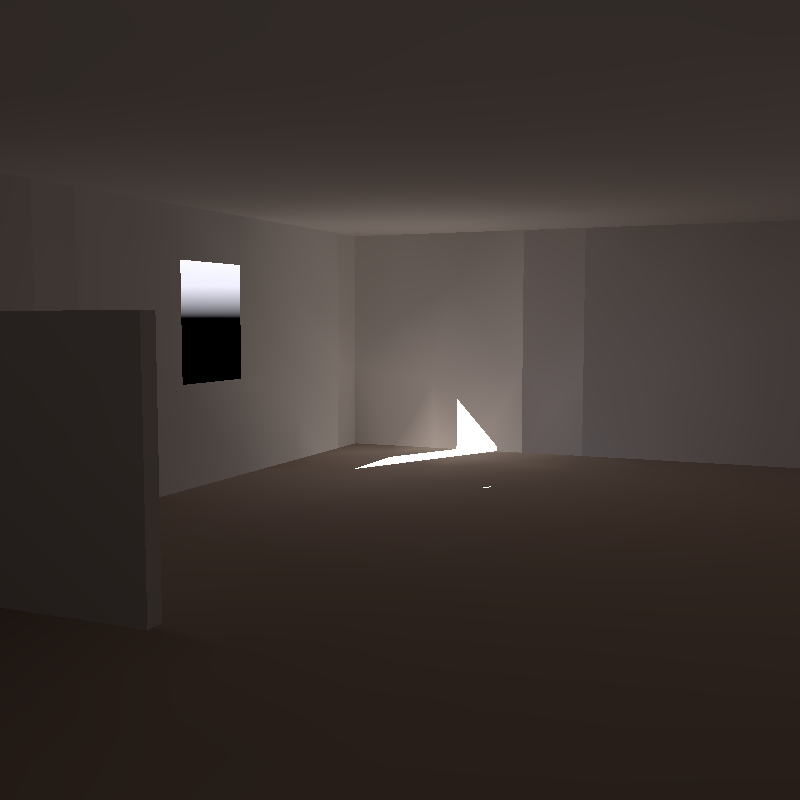
\includegraphics[width=1.1in]{images/renderings/ground_truth/mrc331_camera_chris_march.png} \hfill  %GT
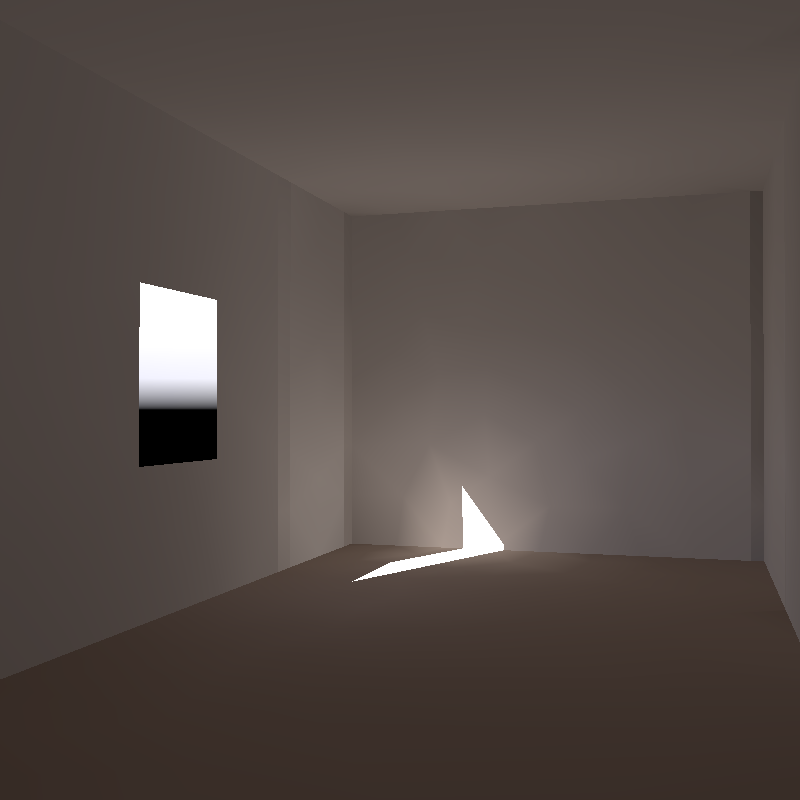
\includegraphics[width=1.1in]{images/renderings/renovations/065_camera_chris_march.png} \hfill %A1
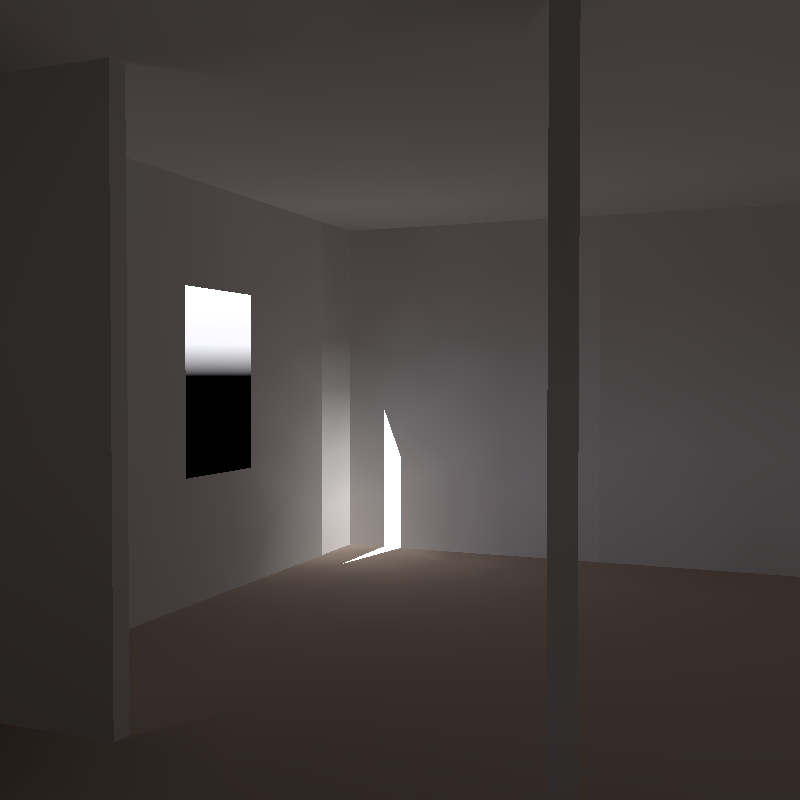
\includegraphics[width=1.1in]{images/renderings/renovations/038_camera_chris_march.png} \hfill   %A2
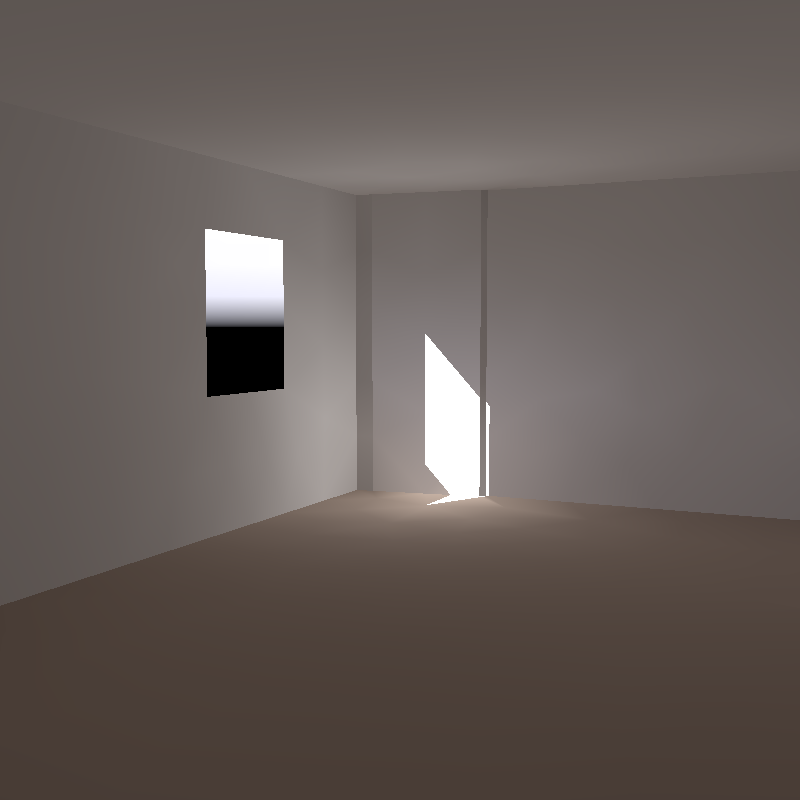
\includegraphics[width=1.1in]{images/renderings/renovations/042_camera_chris_march.png} \hfill   %A3
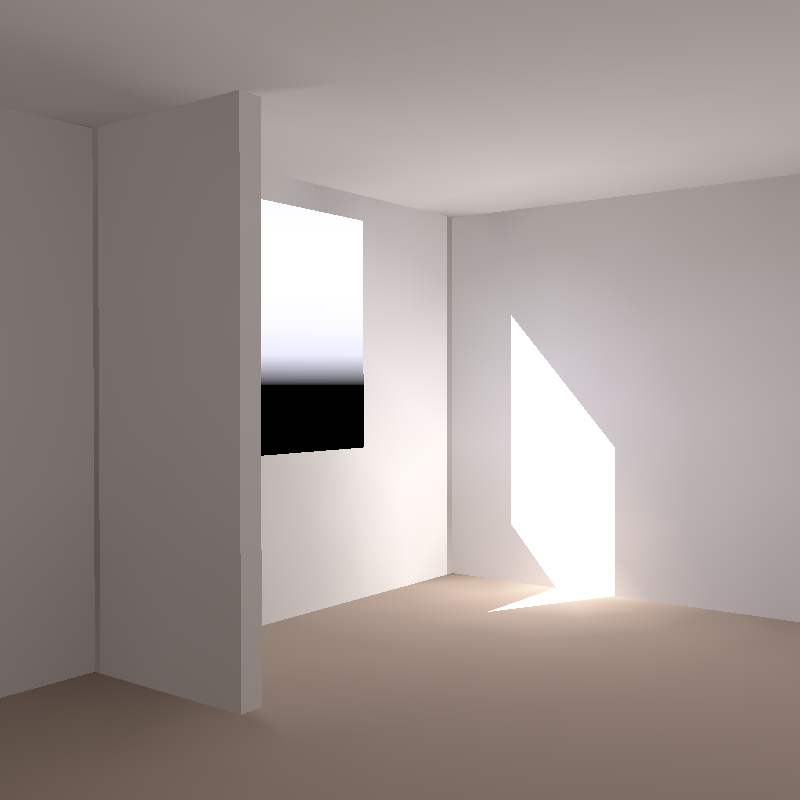
\includegraphics[width=1.1in]{images/renderings/renovations/031_camera_chris_march.png} \hfill   %A4
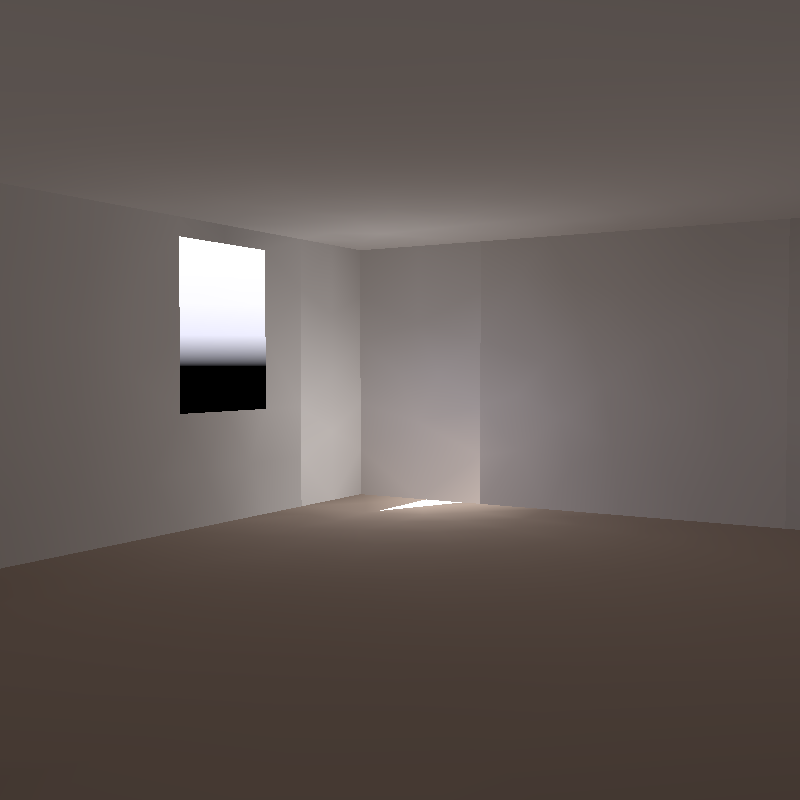
\includegraphics[width=1.1in]{images/renderings/renovations/014_camera_chris_march.png}\vspace{-0.13in}\\   %A5

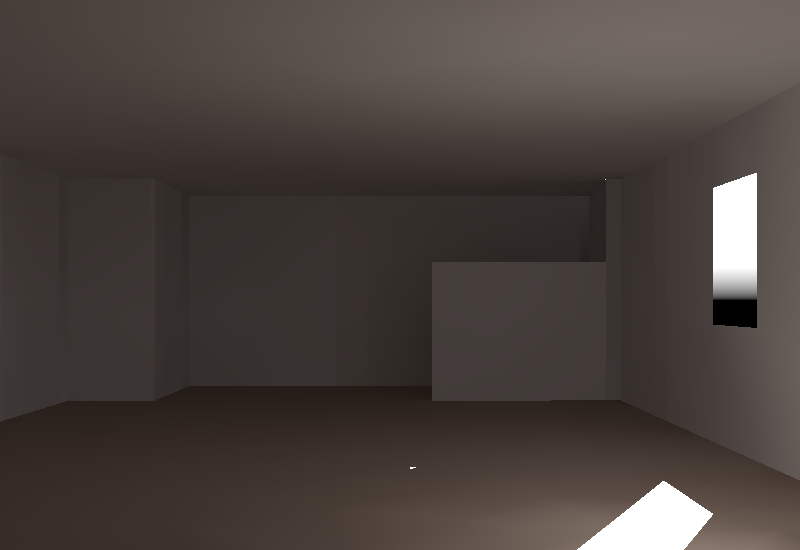
\includegraphics[width=1.1in]{images/renderings/ground_truth/mrc331_camera_dark_march_crop.png} \hfill %GT
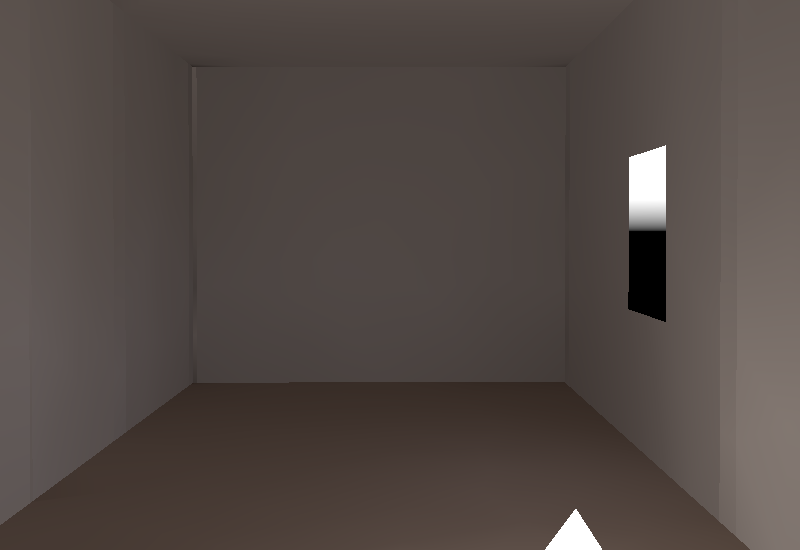
\includegraphics[width=1.1in]{images/renderings/renovations/065_camera_dark_march_crop.png} \hfill %A1
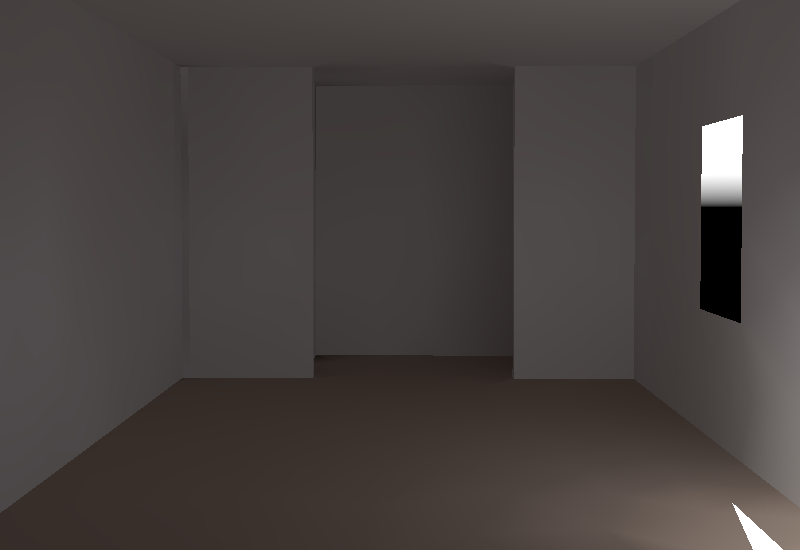
\includegraphics[width=1.1in]{images/renderings/renovations/038_camera_dark_march_crop.png} \hfill %A2
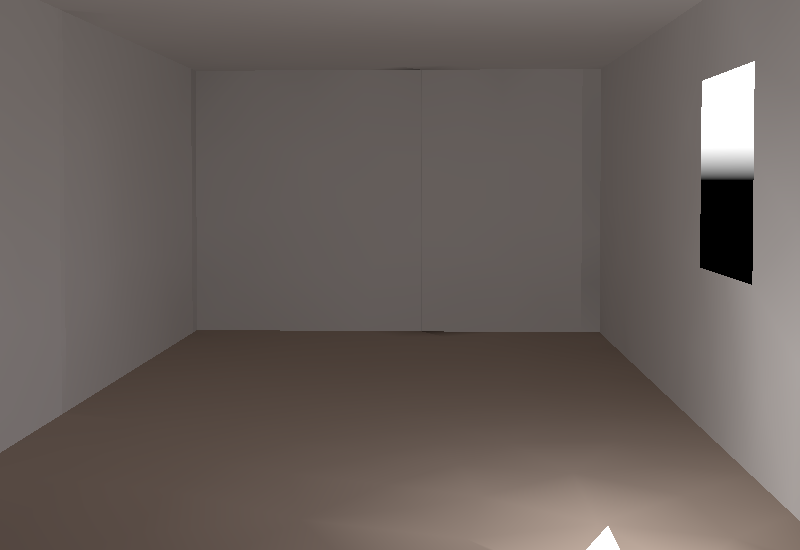
\includegraphics[width=1.1in]{images/renderings/renovations/042_camera_dark_march_crop.png} \hfill %A3
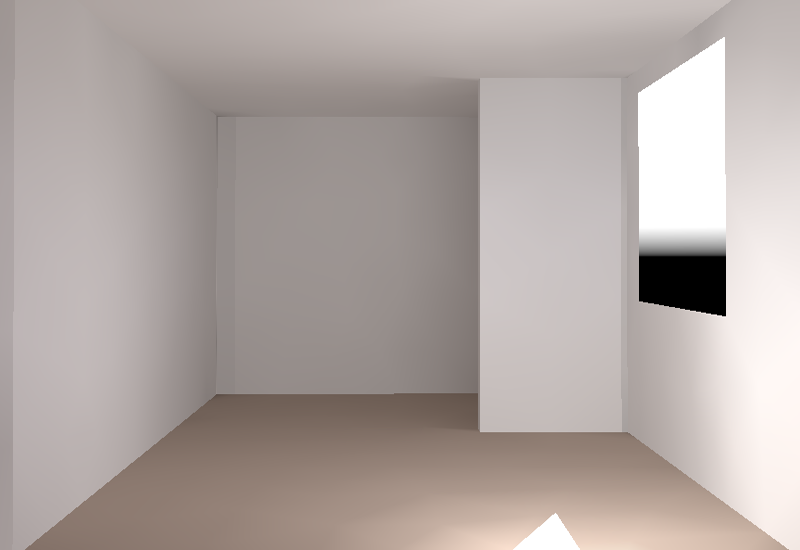
\includegraphics[width=1.1in]{images/renderings/renovations/031_camera_dark_march_crop.png} \hfill %A4
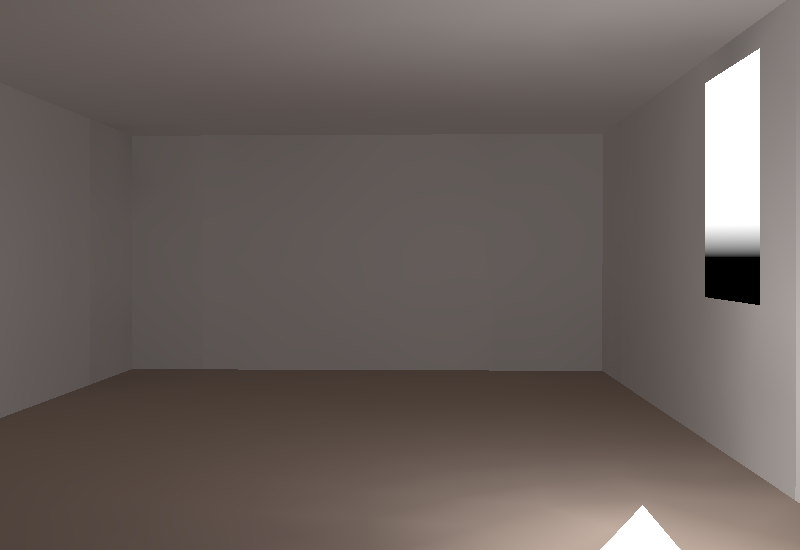
\includegraphics[width=1.1in]{images/renderings/renovations/014_camera_dark_march_crop.png} \\ %A5

\vspace{-2.04in}
\begin{minipage}{1.1in}~{\color{white}{\bf ground-truth}}\end{minipage} \hfill
\begin{minipage}{1.1in}~{\color{white}{\bf A1}}\end{minipage} \hfill
\begin{minipage}{1.1in}~{\color{white}{\bf A2}}\end{minipage} \hfill
\begin{minipage}{1.1in}~{\color{white}{\bf A3}}\end{minipage} \hfill
\begin{minipage}{1.1in}~{\color{white}{\bf A4}}\end{minipage} \hfill
\begin{minipage}{1.1in}~{\color{white}{\bf A5}}\end{minipage} \\
\vspace{1.67in}

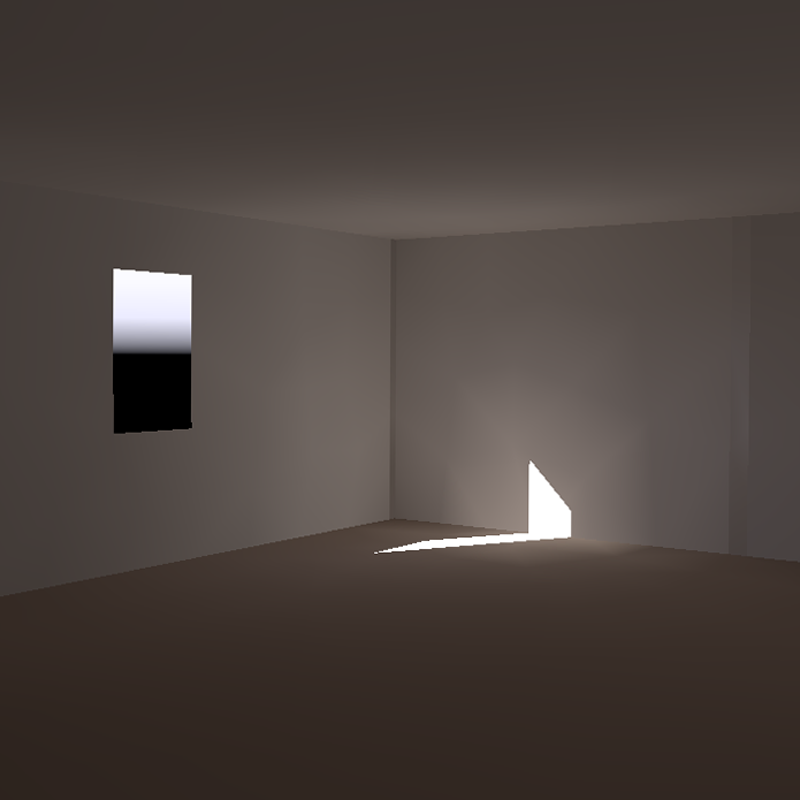
\includegraphics[width=1.1in]{images/renderings/renovations/063_camera_chris_march_crop.png} \hfill   %N1
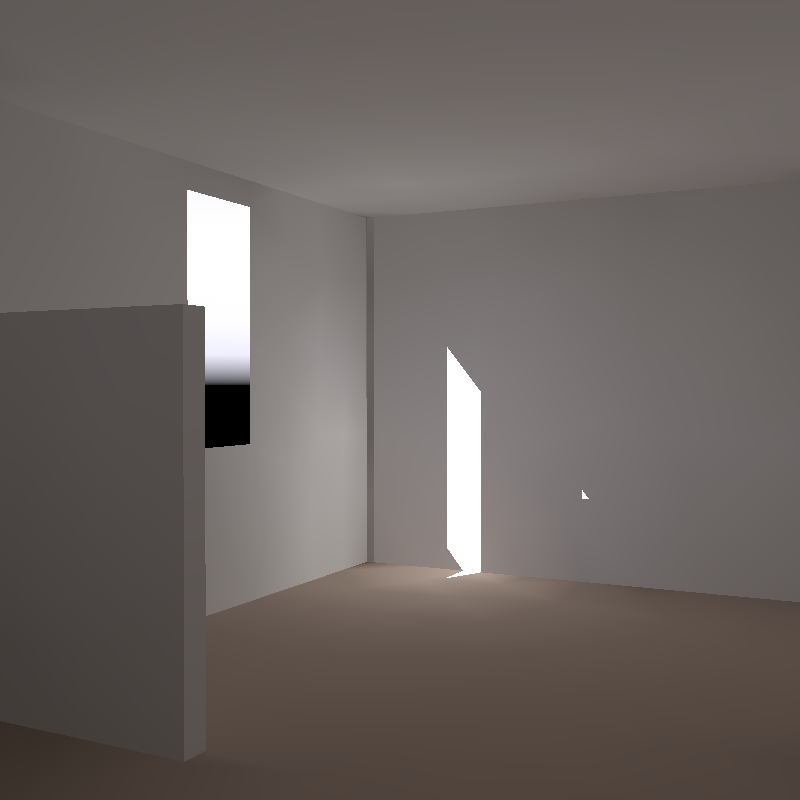
\includegraphics[width=1.1in]{images/renderings/renovations/050_camera_chris_march.png} \hfill   %N2
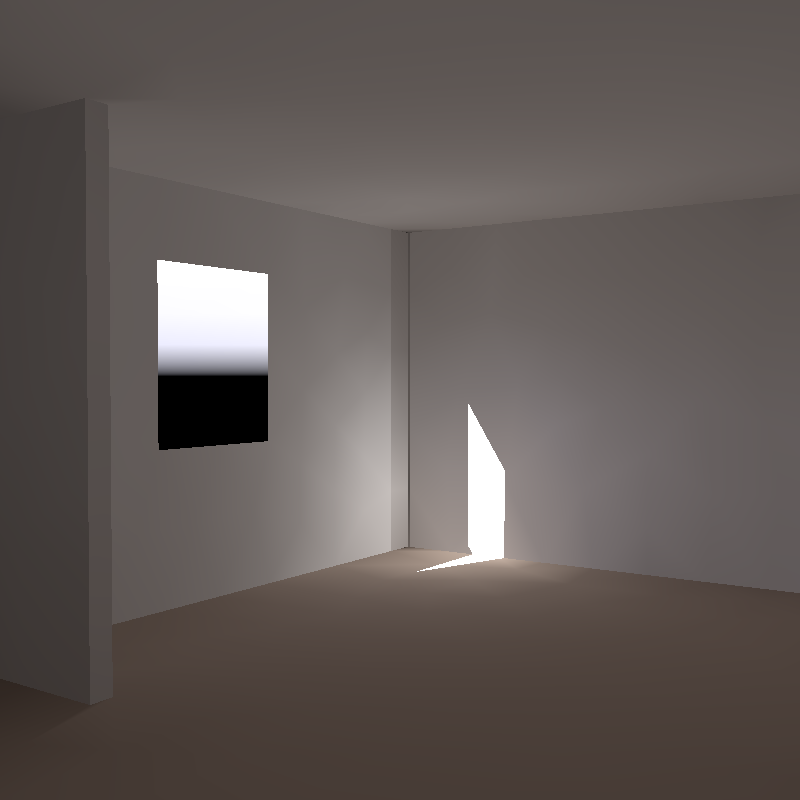
\includegraphics[width=1.1in]{images/renderings/no_renovations/070_camera_chris_march.png} \hfill        %N3
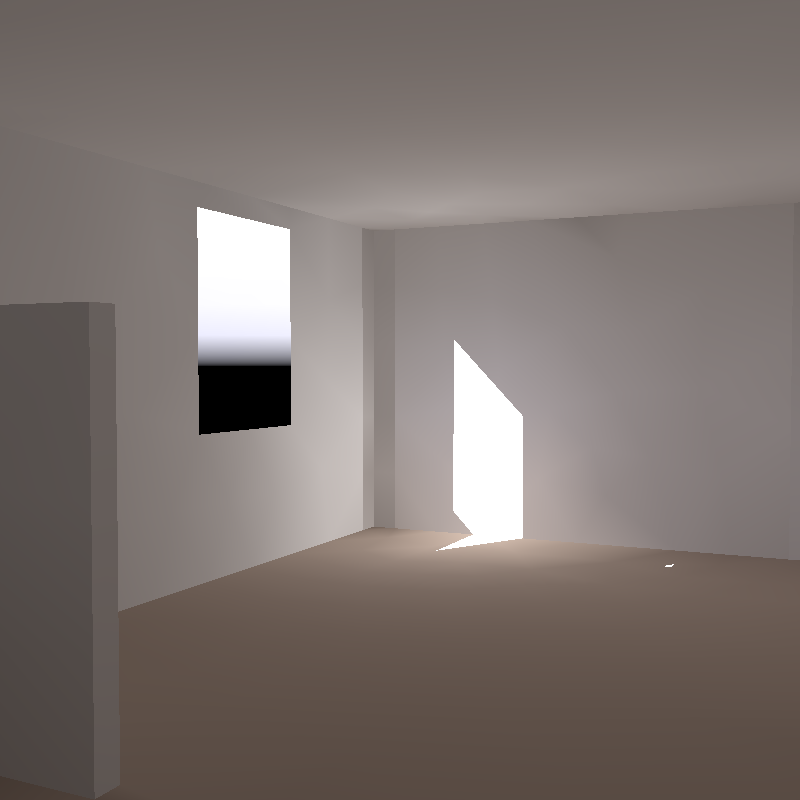
\includegraphics[width=1.1in]{images/renderings/renovations/098_camera_chris_march.png} \hfill   %N4
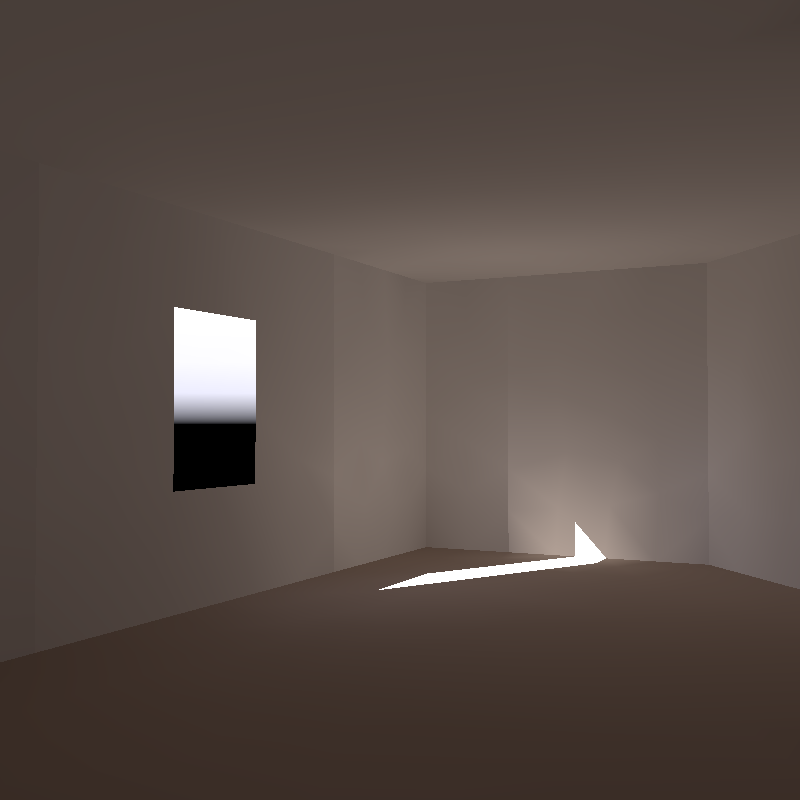
\includegraphics[width=1.1in]{images/renderings/no_renovations/user_085_camera_chris_march.png} \hfill   %N5
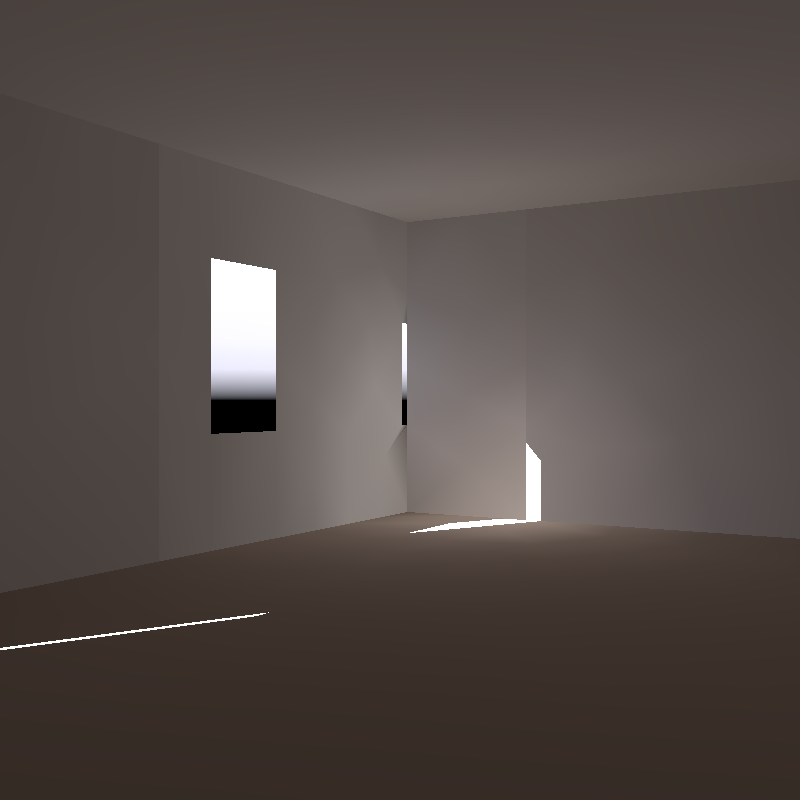
\includegraphics[width=1.1in]{images/renderings/renovations/user_046_camera_chris_march.png}\vspace{-0.13in}\\   %N6

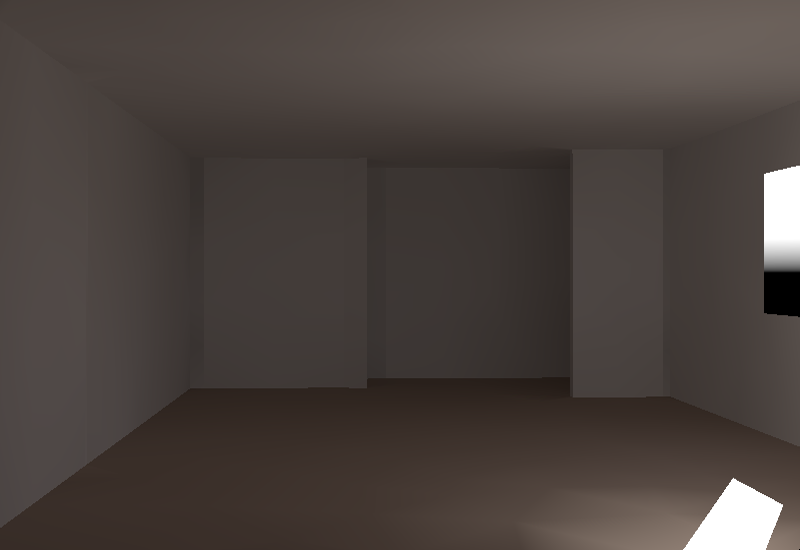
\includegraphics[width=1.1in]{images/renderings/renovations/063_camera_dark_march_crop.png} \hfill    %N1
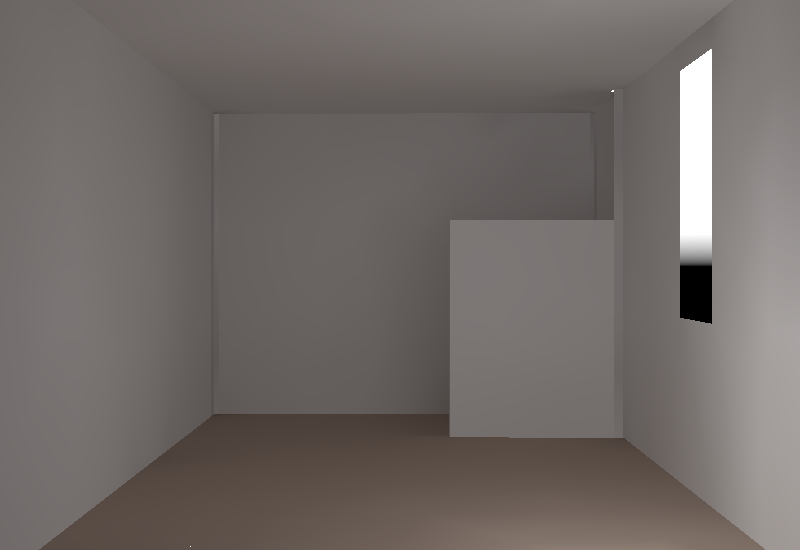
\includegraphics[width=1.1in]{images/renderings/renovations/050_camera_dark_march_crop.png} \hfill    %N2 BARB
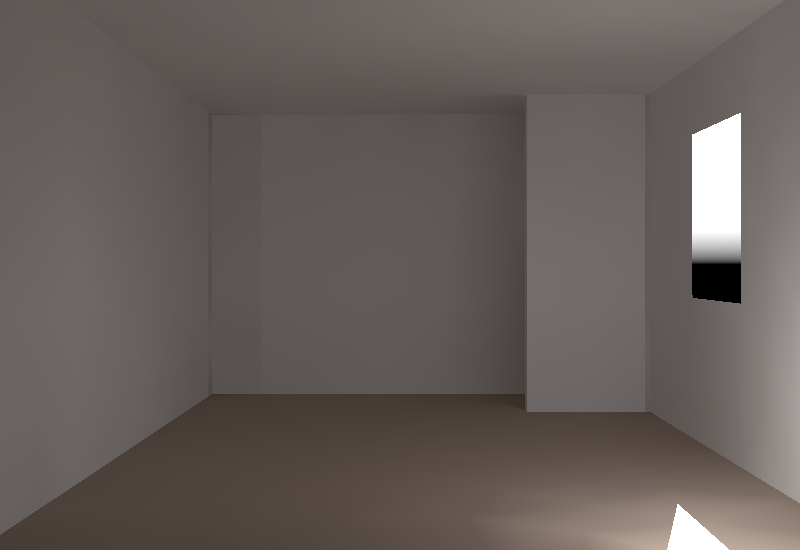
\includegraphics[width=1.1in]{images/renderings/no_renovations/070_camera_dark_march_crop.png} \hfill         %N3
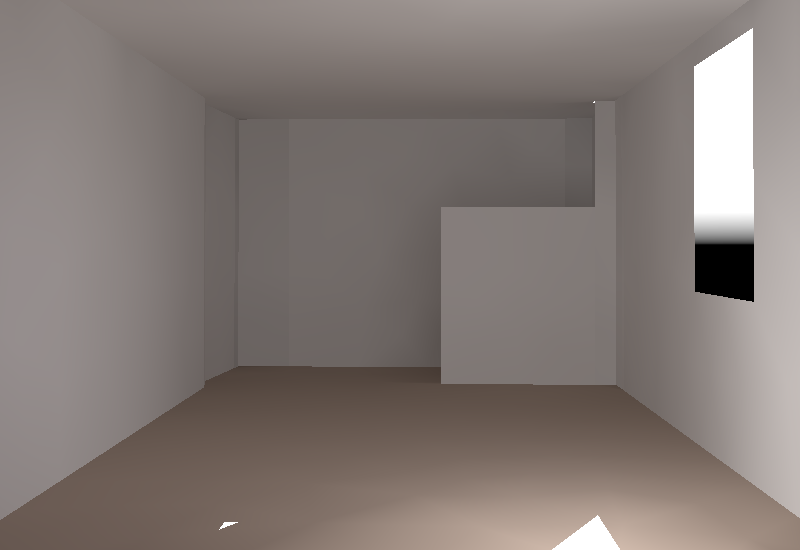
\includegraphics[width=1.1in]{images/renderings/renovations/098_camera_dark_march_crop.png} \hfill    %N4
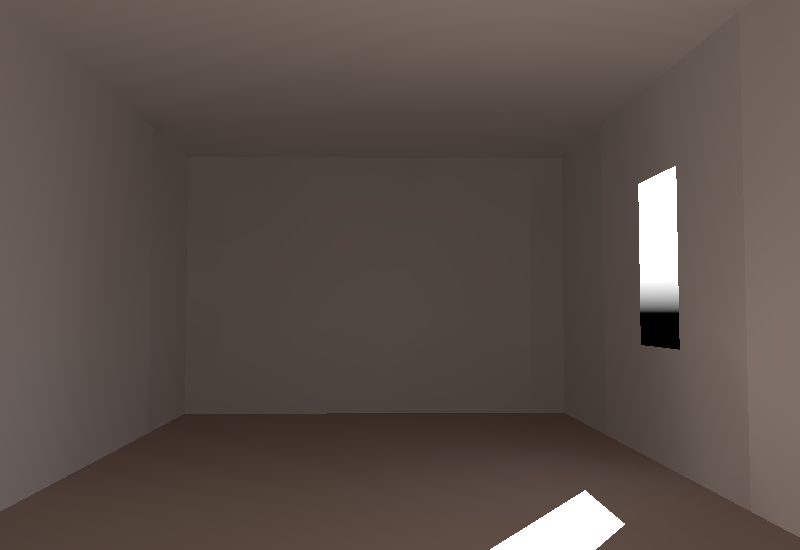
\includegraphics[width=1.1in]{images/renderings/no_renovations/user_085_camera_dark_march_crop.png} \hfill    %N5
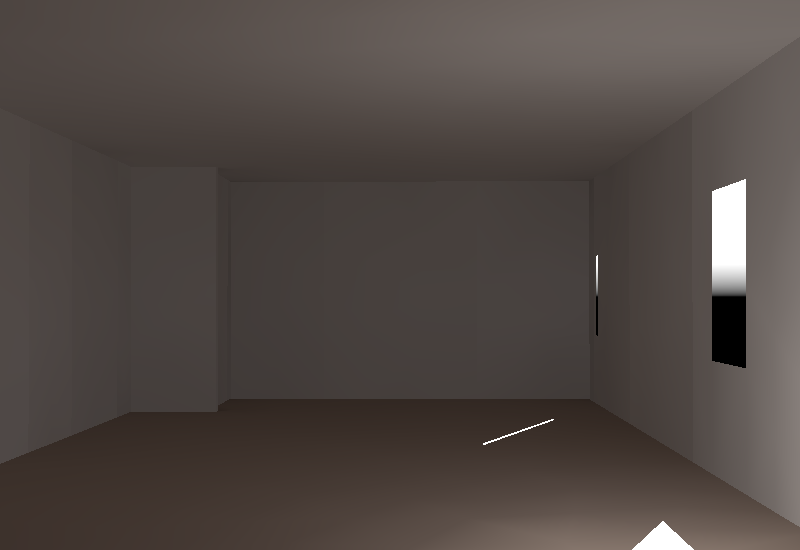
\includegraphics[width=1.1in]{images/renderings/renovations/user_046_camera_dark_march_crop.png} \\   %N6
%\fbox {barb fix! needs crop}

\vspace{-2.04in}
\begin{minipage}{1.1in}~{\color{white}{\bf N1}}\end{minipage} \hfill
\begin{minipage}{1.1in}~{\color{white}{\bf N2}}\end{minipage} \hfill
\begin{minipage}{1.1in}~{\color{white}{\bf N3}}\end{minipage} \hfill
\begin{minipage}{1.1in}~{\color{white}{\bf N4}}\end{minipage} \hfill
\begin{minipage}{1.1in}~{\color{white}{\bf N5}}\end{minipage} \hfill
\begin{minipage}{1.1in}~{\color{white}{\bf N6}}\end{minipage}
\vspace{1.67in}

\caption{ Simulation results for the original room geometry
  constructed by the study participants shown in
  Figure~\ref{figure:original_designs}.  The ground-truth model was
  constructed with the same tangible interface using the true room
  dimensions.  All models are constructed using the same floor, wall,
  and ceiling materials.  All renderings in this figure are March 21st
  at 8:30am.  The desks in the southwest corner of the room (1st and
  3rd rows) experiences glare at this time.  The east side of the room
  (2nd and 4th rows) is quite dark all year, especially in the
  mornings.  }
\vspace{-0.1in}
\label{figure:renderingsOfOriginalGeometry}
\end{figure*}





%\vspace{-0.05in}
\subsection{Part 1: Intuition of Existing Design}
%\vspace{-0.05in}

The aim of Part 1 of the study was to reveal the participant's
intuition about daylighting and provide the user a basis for
self-evaluation after Part 2.  The study began with a tour of an open
office space seating twelve graduate students with desktop computers and
monitors (Figure~\ref{figure:example_room}).
%
This room was selected because of its simple geometry yet non-uniform
daylighting from a single south-facing window.
%
Portions of the room are gloomily dark while other areas
receive direct illumination on the desk surfaces and computer
monitors.  Thus, this space is a good illustration of the need for
careful daylighting analysis during design to maximize use of
illumination from the sun and sky and minimize glare.

%Users were informed that the space was intended for computer science
%students.  
The user was asked to identify areas in the room with too much or too
little daylighting as well as the locations with glare, and to also
specify the variations with time of day and day of the year.  Once the
user had explored the room, we asked them to draw an annotated sketch
of the room showing poor or problematic natural lighting.  The sketch
allows us to understand the complexity and accuracy of their
daylighting intuitions.  
%Furthermore it provides a baseline for them
%to compare 
%enabled them to evaluate how extensive a knowledge of
%daylighting they had as well as give us a sense of how accurate the
%users perceptions of dimensions were so we had a metric to compare
%against later when using our system.
%
Similarly, the questionnaire for Part 1 focused on the user's
pre-existing understanding of daylighting.  We asked the user to
estimate the space's daylight autonomy as well as the weather conditions and use of electric lighting
in the room at the time they did the study.  This gave us an idea of
their prior knowledge as well as any bias from the specific lighting
conditions during their visit.


%The aim of Part 1 of the study was to reveal the participant's
%intuition about daylighting and provide the user a basis for
%self-evaluation after Part 2.
%This task began with a tour of an open office space seating 12
%graduate students with desktop computers and monitors
%(Figure~\ref{figure:example_room}).
%
%This room was selected because of its simple geometry yet non-uniform
%daylighting from a single south-facing window.
%
%Portions of the room are gloomily dark while other areas
%receive direct illumination on the desk surfaces and computer
%monitors.  Thus, this space a good illustration of the need for
%careful daylighting analysis during design to maximize use of
%illumination from the sun and sky and minimize glare.
%
%Users were informed that the space was intended for computer science
%students.  
%The user was asked to identify areas in the room with too much or too
%little daylighting as well as the locations with glare, and to also
%specify the variations with time of day and day of the year.  Once the
%user had explored the room we asked them to draw an annotated sketch
%of the room showing poor or problematic natural lighting.  The sketch
%allows us to understand the complexity and accuracy of their
%daylighting intuitions.  
%Furthermore it provides a baseline for them
%to compare 
%enabled them to evaluate how extensive a knowledge of
%daylighting they had as well as give us a sense of how accurate the
%users perceptions of dimensions were so we had a metric to compare
%against later when using our system.
%The questionnaire for Part 1 focused on the user's pre-existing
%understanding of daylighting.  We asked the user to estimate the
%space's {\em daylight factor},\fbox{should we replace factor with autonomy...everywhere?}
% the percentage of normal working hours
%throughout the year that the desks receive sufficient illumination
%%from the sun and sky alone to perform typical office work, as well as the 
%weather conditions at the time they did the study.  This gave us an idea
%of their prior knowledge as well as any bias they may have obtained from visiting
%the room during a time with interesting daylighting.



\begin{figure*}[t]
\begin{minipage}[c]{3.33in}
  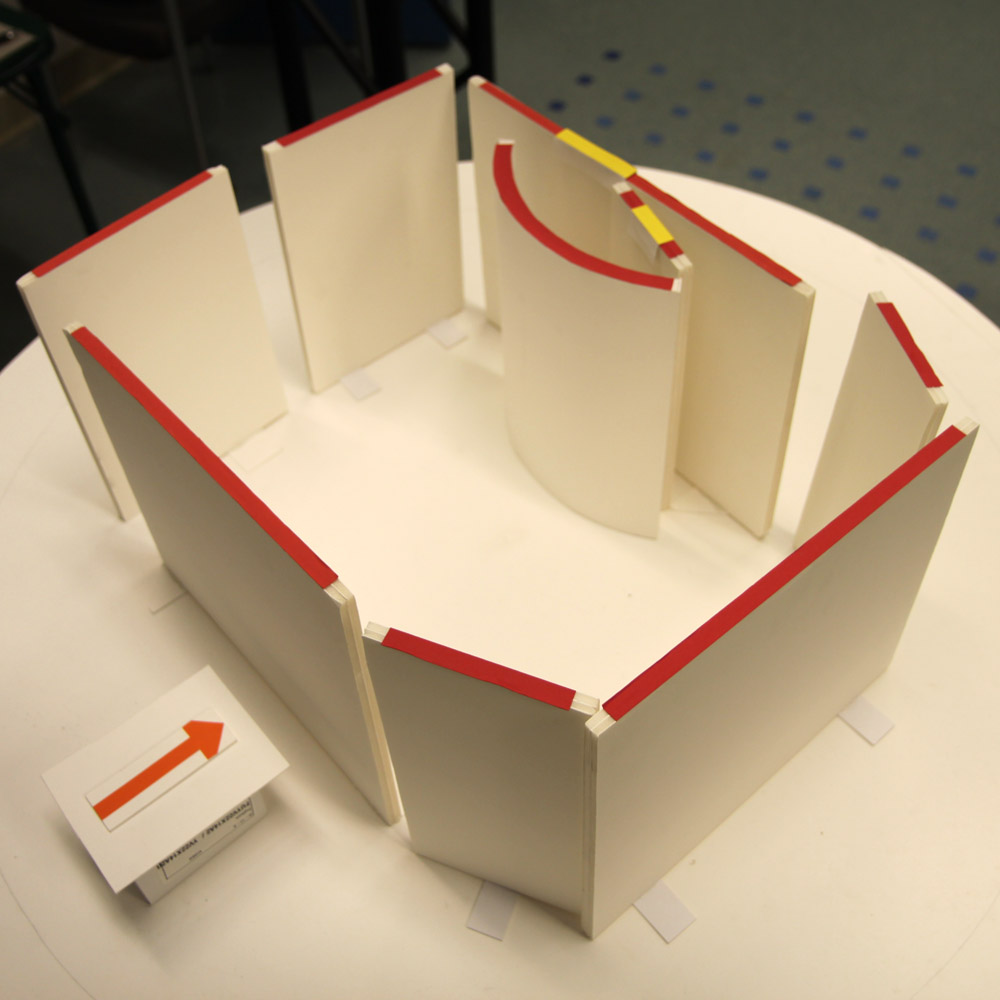
\includegraphics[width=1.65in]{images/photos/38_renovation} %A2
  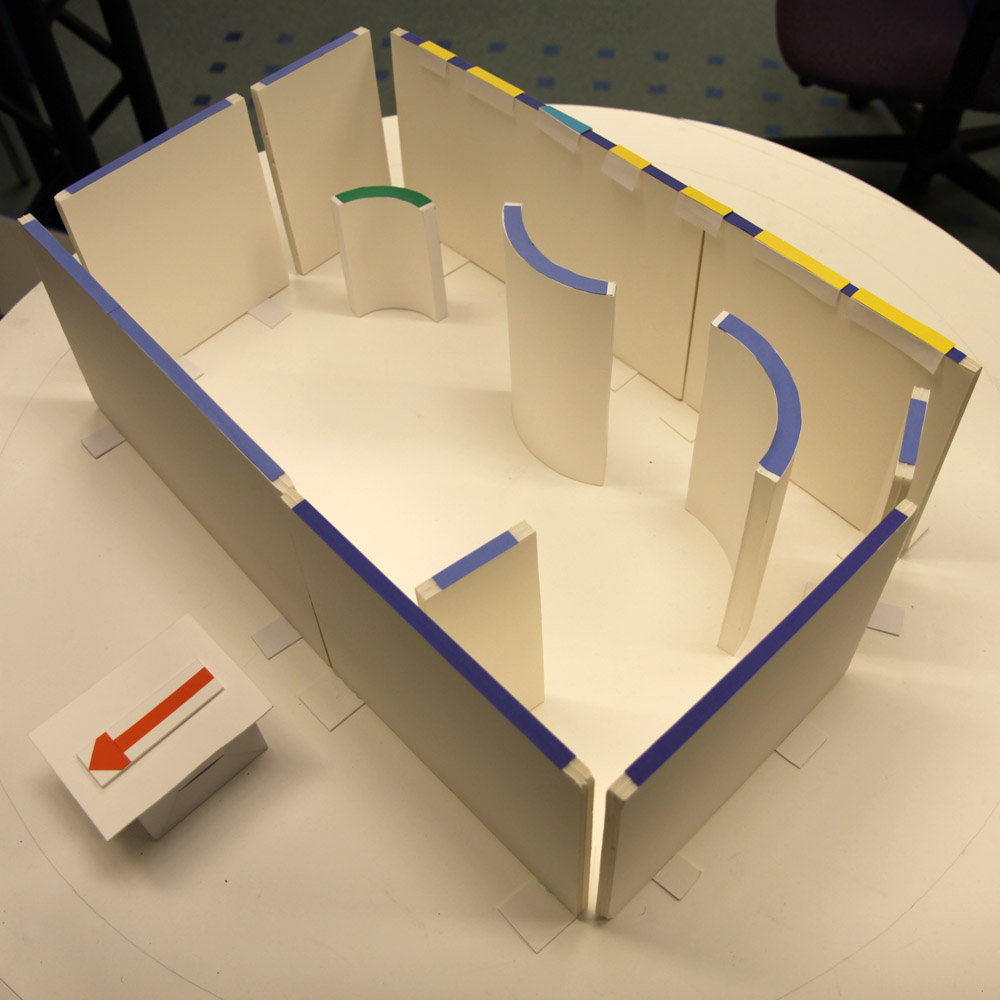
\includegraphics[width=1.65in]{images/photos/42_renovation} %A3
\end{minipage}
\begin{minipage}[c]{4.9in}

  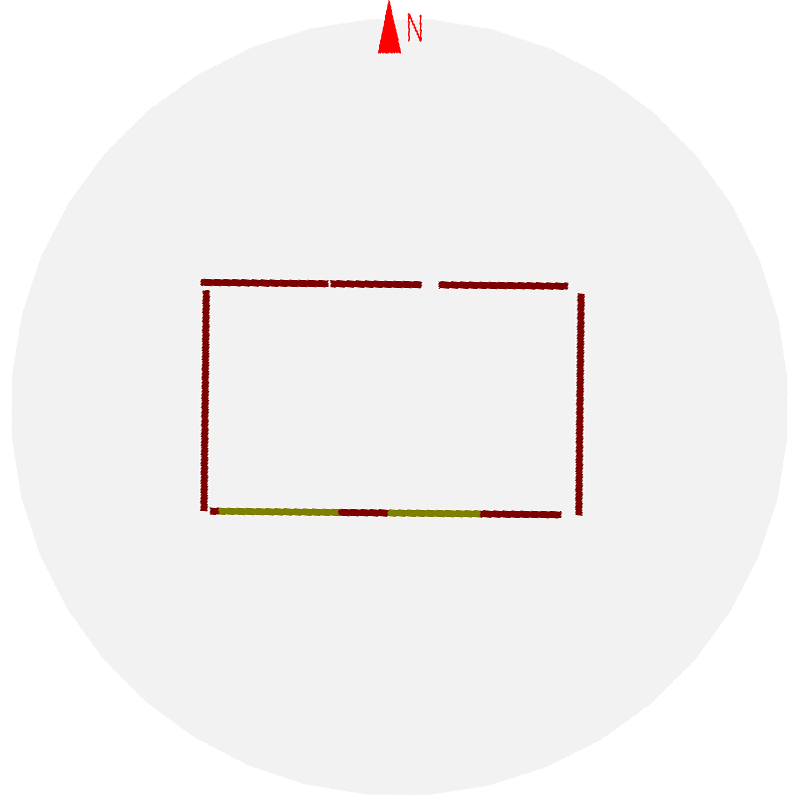
\includegraphics[width=0.9in]{images/section3/0_2D_walls_rotate_edit} %A1
  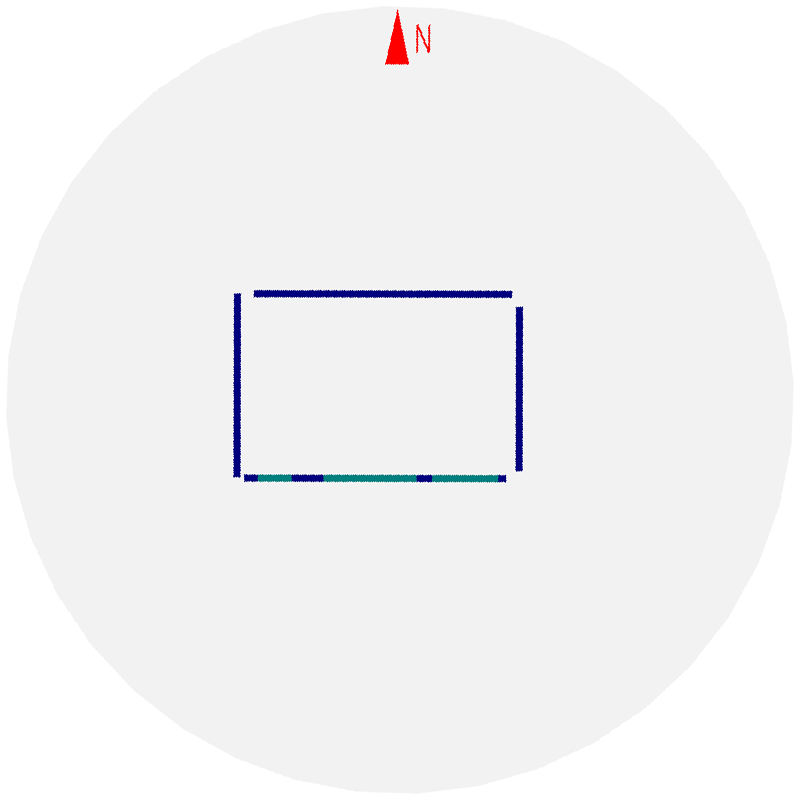
\includegraphics[width=0.9in]{images/section3/6_2D_walls_rotate} %A4
  \includegraphics[width=0.9in]{images/section3/7_2D_walls_rotate} %A5
  \includegraphics[width=0.9in]{images/section3/8_2D_walls_rotate}\\ %A6
  \includegraphics[width=0.9in]{images/section3/2_2D_walls_rotate} %N2
  \includegraphics[width=0.9in]{images/section3/3_2D_walls_rotate} %N3
  \includegraphics[width=0.9in]{images/section3/4_2D_walls_rotate} %N4
  \includegraphics[width=0.9in]{images/section3/9_2D_walls_rotate} %N6
\end{minipage}
\vspace{-1.12in}
\\
\begin{minipage}{1.65in}~\end{minipage}
\begin{minipage}{1.65in}~\end{minipage}
\begin{minipage}{0.9in}{\bf A1}\end{minipage}
\begin{minipage}{0.9in}{\bf A4}\end{minipage}
\begin{minipage}{0.88in}{\bf A5}\end{minipage}
\begin{minipage}{0.88in}{\bf A6}\end{minipage}%
\vspace{0.68in}
\\
\begin{minipage}{1.65in}{\bf ~A2}\end{minipage}
\begin{minipage}{1.65in}{\bf ~A3}\end{minipage}
\begin{minipage}{0.9in}{\bf N2}\end{minipage}
\begin{minipage}{0.9in}{\bf N3}\end{minipage}
\begin{minipage}{0.88in}{\bf N4}\end{minipage}
\begin{minipage}{0.88in}{\bf N6}\end{minipage}\vspace{0.0in}%
  \caption{ In Part 3 of the study participants were asked to propose
    a modest renovation to the geometry to improve the use of
    daylighting.
%Three users came up with especially creative ways to deal with glare in the space.
Renderings of several of these geometries are shown
Figures~\ref{figure:brighter_renovations}~and~\ref{figure:diffusing_renovations}.
  }
\label{figure:improved_designs}
\vspace{-0.1in}
\end{figure*}






\begin{figure*}[t]

\includegraphics[width=1.11in]{images/renderings/renovations/065_camera_chris_march.png} %A1
\includegraphics[width=1.11in]{images/renderings/renovations/065_camera_chris_march_mod.png} %A1
\hfill
\includegraphics[width=1.11in]{images/renderings/renovations/031_camera_chris_march.png}   %A4
\includegraphics[width=1.11in]{images/renderings/renovations/031_camera_chris_march_mod.png}   %A4
\hfill
\includegraphics[width=1.11in]{images/renderings/renovations/063_camera_chris_march.png}   %N1
\includegraphics[width=1.11in]{images/renderings/renovations/063-2_camera_chris_march_mod.png}   %N1

\includegraphics[width=1.11in]{images/renderings/renovations/065_camera_dark_december_crop.png} %A1
\includegraphics[width=1.11in]{images/renderings/renovations/065_camera_dark_december_mod_crop.png} %A1
\hfill
\includegraphics[width=1.11in]{images/renderings/renovations/031_camera_dark_december_crop.png} %A4
\includegraphics[width=1.11in]{images/renderings/renovations/031_camera_dark_december_mod_crop.png} %A4
\hfill
\includegraphics[width=1.11in]{images/renderings/renovations/063_camera_dark_december_crop.png} %N1
\includegraphics[width=1.11in]{images/renderings/renovations/063-2_camera_dark_december_mod_crop.png} %N1

\vspace{-1.9in}
\begin{minipage}{1.11in}~{\color{white}{\bf A1 original}}\end{minipage} 
\begin{minipage}{1.11in}~{\color{white}{\bf A1 renovation}}\end{minipage}
 \hfill
\begin{minipage}{1.11in}~{\color{white}{\bf A4 original}}\end{minipage} 
\begin{minipage}{1.11in}~{\color{white}{\bf A4 renovation}}\end{minipage} 
\hfill
\begin{minipage}{1.11in}~{\color{white}{\bf N1 original}}\end{minipage} 
\begin{minipage}{1.11in}~{\color{white}{\bf N1 renovation}}\end{minipage}

\vspace{1.7in}

\caption{To address the general gloominess of the room, participants
  suggest adding more, taller, and/or wider windows on the southern
  wall (Figure~\ref{figure:improved_designs}).  Some participants also
  removed the existing interior wall/partition that was deemed to be
  an obstruction to daylighting.  While these modifications did
  brighten the room considerably, it will also increase the glare
  problems for those working at desks in the path of the light.
  Renderings in the top row are March 21st at 8:30am and the bottom
  row shows December 21st at 3pm.}
\label{figure:brighter_renovations}

\vspace{-0.1in}
\end{figure*}








%\vspace{-0.05in}
\subsection{Part 2: Analysis of Existing Design}
%\vspace{-0.05in}

In Part 2 of the study, users were introduced to the TUI for
daylighting simulation.  First, we had the participant construct a
physical model of the computer lab they had just visited and sketched
in the previous section.  Participants were then asked to use the
simulation visualizations to evaluate the daylighting, requesting one
or more static time or timelapse animations of particular days of the
year.  The aim was to allow users to evaluate the accuracy of their
predictions in Part 1.  Furthermore, by examining their choice of
times and days selected, we can quantify the thoroughness of their
exploration, and their understanding of the summer and winter solstice
and the fall and spring equinox, and sunrise and sunset.

In addition to the comparing the simulations with their earlier
predictions, the questionnaire for this section also asked them to
re-estimate the daylight autonomy of the space.  Finally, we asked them
to discuss their understanding and perception of the simulation
display.  Collectively the first two parts of the study were designed
to provide insight into the value of our tool as an educational
interface as it evaluates users' perceptions both before and after
utilizing the tool to evaluate daylighting within a simple geometry
that they had personally visited.







\begin{figure*}[t]

\includegraphics[width=1.11in]{images/renderings/renovations/050_camera_chris_march.png}   %N2
\includegraphics[width=1.11in]{images/renderings/renovations/050_camera_chris_march_mod.png}  \hfill %N2
\includegraphics[width=1.11in]{images/renderings/renovations/user_046_camera_chris_march.png}   %N6
\includegraphics[width=1.11in]{images/renderings/renovations/user_046_camera_chris_march_mod.png} \hfill  %N6
\includegraphics[width=1.11in]{images/renderings/renovations/042_camera_chris_december}    %A3
\includegraphics[width=1.11in]{images/renderings/renovations/042_camera_chris_december_mod}    %A3

\includegraphics[width=1.11in]{images/renderings/renovations/050_camera_dark_december_crop.png} %N2
\includegraphics[width=1.11in]{images/renderings/renovations/050_camera_dark_december_mod_crop.png} \hfill %N2
\includegraphics[width=1.11in]{images/renderings/renovations/user_046_camera_dark_march_crop.png}    %N6
\includegraphics[width=1.11in]{images/renderings/renovations/user_046_camera_dark_march_mod_crop.png}  \hfill   %N6
\includegraphics[width=1.11in]{images/renderings/renovations/042_camera_dark_december_crop.png} %A3
\includegraphics[width=1.11in]{images/renderings/renovations/042_camera_dark_december_mod_crop.png} %A3

\vspace{-1.9in}
\begin{minipage}{1.11in}~{\color{white}{\bf N2 original}}\end{minipage} 
\begin{minipage}{1.11in}~{\color{white}{\bf N2 renovation}}\end{minipage}
 \hfill
\begin{minipage}{1.11in}~{\color{white}{\bf N6 original}}\end{minipage} 
\begin{minipage}{1.11in}~{\color{white}{\bf N6 renovation}}\end{minipage} 
\hfill
\begin{minipage}{1.11in}~{\color{white}{\bf A3 original}}\end{minipage} 
\begin{minipage}{1.11in}~{\color{white}{\bf A3 renovation}}\end{minipage}
\vspace{1.7in}

\caption{Only a few of the participants suggested renovations that
  attempt to mitigate the glare problems in the space through new
  geometry in the model.  These proposals involve the addition of
  partitions that diffusely redirect the harsh direct southern light
  for more usable daylighting.
%
}
\label{figure:diffusing_renovations}
\vspace{-0.1in}
\end{figure*}



%\vspace{-0.05in}
\subsection{Part 3: Analysis of a Proposed Renovation}
%\vspace{-0.05in}

The third section involved the use of the tool as a design interface,
rather than just for analysis.  The participants were asked to propose
a ``modest'' renovation of the existing space to improve the use of
daylighting.  This exercise allows us to test if users can effectively
and efficiently make incremental design changes in response to
daylighting needs.  In the spirit of a cognitive walkthrough, few
constraints were placed on the specific edits.  For example, the
participants could move and add windows (as long as they were still on
exterior walls) and they could add interior walls.  Once again the
users were free to explore their new design through daylighting
simulations of their choosing.  Users were permitted to further modify
their design until satisfied with the daylighting in the revised
model.

The short questionnaire at the end of Part 3 asked users to provide
the rational behind their renovation and to estimate the daylight
autonomy of the new space.  To better understand the users' experiences,
a series of questions requesting the users' opinion on the tool's
ability to help users evaluate illumination, determine the potential
for glare, understand the qualities of daylighting, and teach
daylighting concepts.


%\fbox{4.4 was here}
\begin{comment}
\vspace{-0.05in}
\subsection{Part 4: Analysis of a New Design}
\vspace{-0.05in}

The final stage of the study opened the tool to the participants full
creativity.  The user was simply instructed to create a brand new
space to serve the same group of students, but could be situated
anywhere on campus, in an existing or brand new building.  
%For this
%design users were permitted to use curved walls and multiple types of
The participant was encouraged to request daylighting visualization
during the design process enabling them to creatively experiment with
the tool for uncommonly-shaped spaces.

The questionnaire for this section explored the user's motivation
behind the new design, the expressiveness of the physical primitives
for capturing the essential details of the intended design, and the
users estimate of the daylighting autonomy of the new design.  The
intent of Part 4 was both to test if users could freely express an
intended design as well as to see if given complete freedom users were
able to create a space that demonstrated good daylighting
fundamentals.
\end{comment}

%\vspace{-0.05in}
\section{User Study Results}
%\vspace{-0.05in}


Users proved to have different styles of design in the study: both in style 
of design and methods of daylighting.  Architects and non-architects alike 
appeared to come into the study with varying levels of daylighting intuition.


%\vspace{-0.05in}
\subsection{Part 1: Intuition of Existing Design}
%\vspace{-0.05in}

An important concept in understanding and evaluating
daylighting is the sun's height and track across the sky for different
seasons.  The two extremes happen on the solstices. The
sun reaches the highest point in the sky (angle to the horizon) during the summer
solstice (June 21).  The winter solstice
(December 21) is the day the sun reaches the lowest point in the sky
at mid-day.  March 21 and September 21 are the equinoxes, which are
the days when day and night are almost exactly equal.  The sun's track
from east to west across the sky, goes across the southern sky.  This
means that direct light in buildings is obtained from south facing
windows.  Furthermore, direct sunlight will reach much further into a
space from a southern facing window in the winter.
%
From experience, we know that the case study computer lab
(Figure~\ref{figure:example_room}) has some very specific lighting issues.
The desk closest to the window has significant over-illumination as
well as glare issues for the morning hours, which are especially
problematic in the winter.  The far side of the room is consistently
under-illuminated.  The desks in the center of the room suffer from
substantial glare issues, those facing away from the window suffer
from glare on the monitors, while the ones facing towards the window
have glare because the window is so much brighter than the monitors.
The east (left) side of the room suffers consistently from
under-illumination because of its distance from the window.  We
compare this knowledge with the analysis done by the users concerning
the lighting in the space.



The users' sketches varied in level of detail and style
(Figure~\ref{figure:sketches}), but users consistently identified
areas of too much and too little daylighting in the room.  Users did
the study at a variety of times in a variety of weather conditions
(cloudy, sunny, etc.), but their results showed no noticeable relation
to these conditions.  Five out of six of the architects identified a
cone shaped area of bright light near the window.  All of the
architects used a 2D {\em plan} view to convey their information.
However, the architects were not consistent in where they identified
problematic areas for glare.  Three of the architects discerned the
desks in the center of the room would have problem with glare.  Most
users recognized that the desks near the window would be very bright,
but only three of the architects recognized glare being a problem in
this area.  Architects in general seem to have a pretty good idea of
the approximate area lit by a window, but have difficulties discerning
how bad glare will be and when it will be a problem.  One architect
claimed the worst over-illumination would occur in the summer.  This
intuition was exactly opposite of the true lighting condition at
midday.

The style of the non-architects' drawings were more varied. Two of the
seven used 3D perspective drawings to sketch the room.  The
non-architects did not specifically identify a cone-shaped area of
over-illumination near the window.  In general, the non-architects'
sketches provided similar detail of problematic lighting areas.  Their
intuition about lighting concepts also seemed to be of a similar depth
and accuracy.  In fact, one user from each category (architect and
non-architect) demonstrated correct intuition in which areas would be
problems at various points throughout a given day.  While this is a
fairly small sample size, it appeared that these particular
architecture students' training (at least in the first two years)
about daylighting may be fairly limited.





%\vspace{-0.05in}
\subsection{Part 2: Analysis of Existing Design}
%\vspace{-0.05in}

First we evaluate the accuracy of the model construction.
Table~\ref{table:measurements} presents a detailed comparison of the
absolute and relative dimensions of the models built by the
participants in Part 2 of the study
(Figure~\ref{figure:original_designs}).  
%
Users were provided with the rough measurements of the lab (24' x 34'
and 10' tall).  The suggested scale for the physical sketching
environment is 1/12 scale (so 1' in the real world would be 1'' in the
model) and the participants are told that the blue edged walls are 8''
tall, the red edges walls are 10'', and the small green walls are 5''
tall.
%
While eight out of thirteen users made a 8'' tall model, this fact is
not significant because the propagation of light is the same at
different scales.  Furthermore, several users specifically selected
the smaller scale because there were more total 8'' primitives than
10'' primitives.
%While eight out of thirteen users made a 8 inch tall model, we decided
%it was not significant because multiple users requested to use a
%slightly different scale due to there being more 8 inch primitives
%available than 10 inch primitives. Note that size does not matter as
%light will interact the same on different scales.
%


Overall, users were relatively accurate (within 15\%) with the
dimensions of the outer walls and with the placement of the window on
the wall.  Users were less accurate in the ratio of the height to
wall.  Because the windows are proportional to the height of the wall
in our program, this has a direct affect on the amount of light in the
room.  The 24\% misestimation of the architects and the 19\% error of
the non-architects will result in simulations that are noticeably 
brighter or darker than the ground truth.
%
Users were surprisingly inaccurate with the length of the window in
relation to the size of the wall.  Non-architects overestimated the
size by 19\% whereas architects overestimated the size by 54\% (only
21\% if the worst outlier is removed).  While users seem to have
compensated their errors on the width of the window with the height of
the wall, it is notable that users did not more carefully observe the
dimensions of the window.  Also, because the window appeared to often
be the wrong shape, the lighting will less accurate.

Global illumination renderings of the geometry created in Part 2 of
the study are presented in
Figure~\ref{figure:renderingsOfOriginalGeometry}.  All models
correctly capture the problem with glare in the southwest corner of
the room in the morning.  However the variation in brightness and
distribution of light within the space, compared to the ground truth,
does indicate the relative importance and negative impact of geometric
errors in the modeling process.


As this was the users' first experience with the TUI daylighting tool,
most users requested 5-10 different daylighting simulations.  Most
users chose to view a winter date, a summer date, and one or both of
the fall and spring equinoxes.  Two architects and two non-architects
chose the solstices within a couple days.  Others mostly chose dates
across the seasons.  All users recognized the importance of requesting
multiple dates throughout the year.  Some users were familiar with the
seasonal patterns while others demonstrated a confusion as to when the
extremes occurred: two architects expressed confusion between the
equinoxes and the solstices.  After playing with the tool, most users
solidified their understanding of seasonal daylight patterns, although at
least one user, architect A6, failed to grasp this concept.  In Part
2, many users appreciated the complex visualization the tool provided,
allowing them to better evaluate parts of the room that had
significant glare.  Although users still had a large range (30\% to
90\%) in their opinions of the daylight autonomy users changed their
original estimations by an average absolute value of 20\% from their
original estimate.  This shows that users impression of daylighting in
this space were positively influenced by the use of the tool, even
though their perceptions of lighting still varied widely.




Participants were asked on the questionnaire: ``What new insights did
you gain about daylighting within the space?  Were any of the
simulation results unexpected?''
%
5 out of 6 architects and 6 out of 7 non-architects claimed they
gained additional daylighting insight from this first task.  A1 said
``I learned there was much more light shed on the west wall than I
expected, and was less light on the north and east walls, especially
on the north."  User A2 was surprised by the sun's penetration into
the room: ``New insights would be that the room's depth is rather
shallow in the winter months when the sun is low, allowing the light
to cause a significant amount of glare all the way across the room."
Not only did users find areas of problem lighting but users who
requested the most simulations also were able to identify problem
times.  Participant A5 said ``I learned how the sun's direction
relative to the date and time is a huge factor since I also saw March
20 from noon to 6 PM to see the difference.''  Interestingly, some
users claimed that the tool helped them remember things about lighting
which they hadn't remembered correctly when evaluating without the
tool: ``I forgot to take into account that during the summer the sun
is higher up, so actually less light penetrates throughout the room.''
Non-architects remarked on what they learned as well, but most of them
offered more generic remarks.  N6 commented: ``I gained additional
insight into how the lighting changes throughout the day, and at
different times in the year.  I was then able to compare them with
each other to see the tendencies of the lighting in the room.''

Despite some inaccuracies in model dimension and scale, participants
gained quite a bit of insight about the daylighting in the case study
space by using the TUI daylighting tool.  Architects gained specific
insights into where light would fall in the space; non-architects
seemed to gain more general knowledge about the dynamic nature of
daylighting.

%\vspace{-0.05in}
\subsection{Part 3: Analysis of a Proposed Renovation}
%\vspace{-0.05in}

In Part 3 (Figure~\ref{figure:improved_designs}), all but two
participants attempted to get more light into the space by adding
windows or by using multiple smaller windows
(Figure~\ref{figure:brighter_renovations}).  As a result, users
indicated that they were able to achieve a much larger daylight autonomy
averaging 76\% in comparison to an average of 46\% as in Part 2.  Some
users chose to replace most of the entire south-facing wall with
windows, for example A4.  While an effective way to make the room
brighter, only a few users (4 out of 13) made modifications in an
attempt to minimize glare (Figure~\ref{figure:diffusing_renovations}),
which is a significant problem in the current space, even with just
one window.  Both users A2 and A3 tried alternative ways to reduce
glare: using curved walls to diffuse the light into the room.  While
this will effectively balance daylight to reduce glare, it is at the
expense of usable space in the room.  In the example of participant
N2, perhaps the small amount of room taken up by new walls would leave
sufficient space for twelve students, but in the case of A3 we see
that close to 25\% of the space becomes unusable for students by
adding these windows and having additional walls just a few feet away.
Many of the other participants seemed to disregard glare.  We believe
this may be partially because we have not provided sufficient glare
visualization.  We will discuss this further in future work.


%In Part 3 (Figure ~\ref{figure:brighter_renovations}) almost all the
%participants attempted to get more light into the space.  All but two
%users did this by adding windows to the space or by using multiple
%smaller windows.  As a result, users indicated that they were able to
%achieve a much larger daylight factor averaging 76\% in comparison to
%an average of 46\% as in Part 2.  Some users chose to replace most of
%the entire south-facing wall with windows, for example A4.  While an
%effective way to make the room brighter, only a few users (4 out of
%13) made modifications in an attempt to minimize glare (Figure
%~\ref{figure:diffusing_renovations}), which is a significant problem
%in the current space, even with just one window.  Both users A2 and A3
%tried alternative ways to reduce glare.  They used curved walls to
%diffuse the light into the room While this will effectively balance
%daylight to reduce glare, it is at the expense of usable space in the
%room.  In the example of participant N2, perhaps the small amount of
%room taken up by these new walls would leave sufficient space for 12
%students, but in the case of A3 we see that close to 25\% of the space
%becomes unusable for students by adding these windows and having
%additional walls just a few feet away. Many users seemed to disregard
%glare.  We believe this may be partially because we have not provided
%sufficient glare reduction techniques.  We will discuss this further
%in future work.


%\fbox{5.4 was here}
\begin{comment}
\vspace{-0.05in}
\subsection{Part 4: Analysis of a New Design} 
\vspace{-0.05in}

In Part 4 of the study, users utilized the freedom of an open design
exercise resulting in more varied shapes and designs than in the
previous sections \fbox{remove reference?}(Figure 6).  Despite the users having much more flexibility in
Part 4 than in Part 3, users reported daylight autonomy estimates that were very
similar for the two parts.  Users thought that the daylight autonomy of
their final design was on average 77\%.  Users accomplished this in a
variety of ways, but often as an extension or elaboration of the style
of the renovations they proposed in Part 3.  Overall, participants
spent much more time with Part 4 than the earlier sections.  Although
the participants did not request as wide a variety of simulation times
for Part 4, they did use the simulation tool more frequently in
revising their open-ended design. We expect user spent more time on
this exercise because we gave them the most freedom.
% times were often requested more
%frequently as users' designs evolved based upon the lighting.  
Users frequently experimented with curved walls in this exercise.  One
user stated how they were trying to use a curved wall to redistribute
light within the space.  Figure\fbox{remove reference?} 6 illustrates how participants
utilized many windows to get sufficient natural lighting in the room.
However, it was clear that users still did not fully appreciate the
problematic aspect of glare.  While five participants (two architects 
and three non-architects) used interior walls to try to redirect light and reduce
glare, the rest had windows which would leave much of the space victim
to large amounts of glare.
\end{comment}

%\vspace{-0.05in}
\subsection{Discussion}
%\vspace{-0.05in}

Many users were excited about the ability to track sunspots on the
floor with this program and thought it useful.  Although users
generally seemed impressed with the tool, the variance in the daylight
autonomy across participants in each exercise implied that users did not
receive an accurate quantitative perception from the system of what
was too much or too little daylighting in the space.
%
Eleven out of thirteen users said they were 
%\fbx{\% check this stat}
surprised or saw results they did not expect in the lighting
simulation.   Many of these comments
involved observing how different the lighting was in the summer
vs. the winter months.  Some users expressed surprise that they had
not realized that with a south facing window at midday it is brighter
in the winter than in the summer.  Others
were surprised by how deep into the room the sunspot reached in the
winter months.
%
Many users were pleased by the ease of modifying designs using the
TUI.  Users consistently expressed that designing was simple and
intuitive.  Users complaints about the system focused on the limited
number of primitives and not that designing was obscure or tedious.
One user commented that the system was limited to one story
simulations and would like a better way to view lighting for the whole
structure.

%Many users were excited about the ability to track sunspots on the
%floor with this program and thought it useful.  Although users
%generally seemed impressed with the tool the variance in the daylight
%factor across participants in each exercise implied that users did not
%receive an accurate quantitative perception of what was too much or
%too little daylighting in the system.
%
%Many of the users (eleven out of thirteen) said they were % check this stat
%surprised or saw results they did not expect in the lighting
%simulation.   Many of these comments
%involved observing how different the lighting was in the summer
%vs. the winter months.  Some users expressed surprise that they had
%not realized that in a South facing room it is possible that during
%mid-day it may be brighter in the winter than in the summer.  Others
%were surprised by how deep into the room the sunspot reached in the
%winter months.
%
%Many users were pleased by the ease of modifying designs using the
%TUI.  Users consistently expressed that designing was simple and
%intuitive.  Users complaints about the system focused on the limited
%number of primitives and not that designing was obscure or tedious.
%One user commented that the system was limited to one story
%simulations and they would like a better way to view lighting for the
%whole structure.

%\vspace{-0.05in}
\section{Limitations and Future work}
%\vspace{-0.05in}

Our current daylighting simulation tool does not output a measurement
of the daylighting effectiveness (e.g., daylight autonomy), thus we
cannot quantitatively or directly compare participants to each other.
We plan to implement and visualize these metrics in future work.  We
also plan to perform a comparison study with our tool and a
traditional computer-based daylighting interface.  This comparison
would investigate the accuracy as well as the speed in accomplishing
daylighting simulations tasks.  The main challenge in a direct
comparison is the steep learning curve for existing modeling and
daylighting software and the difference in purpose for our tool (early
stage design exploration) vs. other tools (late stage design
analysis).  We hypothesize that comparison of the interfaces will
highlight differences both in terms of creativity in designing and
perception of light in the space based on the varying dimensionality.
%
Currently we can only display information if it can be projected onto
a physical element of the model; we cannot visualize the interaction
of daylighting with things such as furniture, unless appropriately
sized physical objects are placed into the model.
%
To address this we would like to investigate additional augmented
reality techniques, for example a handheld viewing
device~\cite{Ishii97tangiblebits:,642613,1517704} to provide a more
detailed window into the virtual space.

This study showed us that while users felt their daylighting intuition
was enhanced by the tool, users still struggled to quantitatively estimate
usable light in the space.  This may be due to the high dynamic range
of actual daylighting and the limited dynamic range of our tabletop
SAR display.  The tool could be modified to use false color and other
visualizations to show problem areas,
e.g., glare regions could be displayed with red arrows.  The system is
limited by the number of primitives available.  Although the system
can deduce that gaps between the walls should be filled, some users
expressed concern that they did not have as many primitives as they
would have liked to complete their designs, especially in the case of
symmetric buildings.
%
Our daylighting simulation and projection system is currently limited
to diffuse material properties.  While this is sufficient to model
most surfaces inside many typical office spaces, as hope to address
this in the future.  The windows also have a simple model, we hope to
replace this so glare can be actively reduced by choosing alternate
styles and materials.


%\vspace{-0.05in}
\section{Conclusion}
%\vspace{-0.05in}

Participants in this study were significantly and positively
influenced by our tangible interface for daylighting simulation.
Users consistently claimed that their lighting intuition was improved,
their design was aided by the tool, and that the interface was
accessible.  Many participants used the tool to look at lighting in
various seasons to understand how daylighting will vary throughout the
year.  Despite this, it was clear that users need additional
quantitative feedback and visualization to more fully analyze glare in
high contrast lighting conditions.  Our results show that users felt
that with a Tangible User Interface they were able to evaluate
daylighting better than with their own intuition alone.  The interface
provides an effective tool for designing the shape of an architectural
space and with extensions could assist users in reducing glare and
selecting window materials as well.


%Despite the fact that there were significant differences in estimation
%of daylight factor across the participants' designs, users were
%significantly and positively influenced by our tangible interface for
%daylighting simulation.  Users consistently claimed that their
%lighting intuition was aided and improved by the tool and that the
%interface was accessible.  Many users used the tool to look at lighting
%in various seasons to get a better idea of how daylighting might affect
%the space at other times in the year.  Despite this, it was clear that 
%one area users need to be educated on more thoroughly before using the tool
%is the parts of the year with the most extreme lighting conditions.
%
%Problems discussed in this paper such as
%lighting accuracy and limited primitives were problems given the
%current implementation of the interface and not limitations that would
%require a different type of interface.  Users often radically changed
%their designs when they observed the initial lighting in a space.  Glare was 
%especially problematic in users' simulations.  While some users could 
%recognize where glare was, it was evident that the system needs to 
%augmented to include some other glare reduction techniques.



%\fbox{JOSH STUFF}
%2 dates: March 21 \@ 8:30am and DEC 21st \@ 3pm


\bibliographystyle{abbrv}
%%use following if all content of bibtex file should be shown
%\nocite{*}
\bibliography{nasmaj}
\end{document}
